\subsubsection{Module MD-01: Quản lý Lịch làm việc (Scheduling)}


\begin{longtable}{|m{2cm}|m{2.5cm}|m{2cm}|m{4cm}|m{4.5cm}|}
\caption{Danh sách Yêu cầu Chức năng cho Module MD-01: Quản lý Lịch làm việc} \label{tab:fr_md01} \\
\hline
\textbf{Mã Module} & \textbf{Mã Yêu cầu CN} & \textbf{Mã Người dùng} & \textbf{Tên Chức năng} & \textbf{Mô tả Ngắn} \\
\hline
\endhead % Header cho các trang tiếp theo

\hline
\endfoot % Footer cho bảng

\hline
\endlastfoot % Footer cho trang cuối cùng

MD-01 & FR-MD01-01 & US-01 & Tạo ca làm việc & Cho phép Quản lý nhà hàng định nghĩa các ca làm việc mới (thời gian bắt đầu, kết thúc, ngày, vai trò cần thiết, số lượng nhân viên cần cho vai trò đó). \\
\hline
MD-01 & FR-MD01-02 & US-01 & Gán nhân viên vào ca & Cho phép Quản lý nhà hàng chỉ định nhân viên cụ thể cho các vị trí trống trong ca làm việc đã tạo, dựa trên vai trò phù hợp của nhân viên. \\
\hline
MD-01 & FR-MD01-03 & US-01 & Xem lịch biểu Gantt & Hiển thị lịch làm việc của tất cả nhân viên hoặc lọc theo vai trò dưới dạng biểu đồ Gantt trực quan theo dòng thời gian (ngày, tuần, tháng). \\
\hline
MD-01 & FR-MD01-04 & US-01 (Trigger), System (Action) & Phát hiện trùng lịch & Hệ thống tự động kiểm tra và đưa ra cảnh báo trực quan (ví dụ: đổi màu ca bị trùng) nếu một nhân viên được gán vào hai ca làm việc có thời gian trùng nhau. \\
\hline
MD-01 & FR-MD01-05 & US-01 & Xuất bản và Thông báo lịch & Cho phép Quản lý nhà hàng công khai (publish) lịch làm việc đã xếp và kích hoạt hệ thống tự động gửi thông báo (ví dụ: email, thông báo trong ứng dụng) đến từng nhân viên về lịch trình cá nhân của họ. \\
\hline
MD-01 & FR-MD01-06 & US-07 & Xem lịch cá nhân & Cho phép Nhân viên xem lịch làm việc đã được xuất bản của riêng mình thông qua cổng thông tin nhân viên hoặc ứng dụng di động. \\
\hline
MD-01 & FR-MD01-07 & US-01 & Sao chép lịch tuần & Cho phép Quản lý nhà hàng sao chép nhanh lịch làm việc của một tuần (hoặc khoảng thời gian tùy chọn) sang tuần kế tiếp để tiết kiệm thời gian lập lịch. \\
\hline
MD-01 & FR-MD01-08 & US-01 & Quản lý vai trò công việc & Cho phép Quản lý nhà hàng định nghĩa các vai trò công việc trong nhà hàng (ví dụ: Bếp trưởng, Phục vụ, Pha chế, Lễ tân) để sử dụng khi tạo ca và gán nhân viên. \\
\hline
MD-01 & FR-MD01-09 & US-07 & Đánh dấu không sẵn sàng & Cho phép Nhân viên (nếu được cấu hình) đánh dấu các khoảng thời gian không sẵn sàng làm việc (ví dụ: nghỉ phép, bận việc riêng) để Quản lý nhà hàng xem xét khi xếp lịch. \\ % Thêm mới dựa trên case study
\hline
MD-01 & FR-MD01-10 & US-01 & Xem lịch theo vai trò & Cho phép Quản lý nhà hàng lọc và xem lịch làm việc chỉ của các nhân viên thuộc một vai trò cụ thể (ví dụ: xem tất cả ca của Bếp trưởng). \\ % Làm rõ FR-MD01-03
\hline

\end{longtable}


\begin{figure}[H]
	\centering
	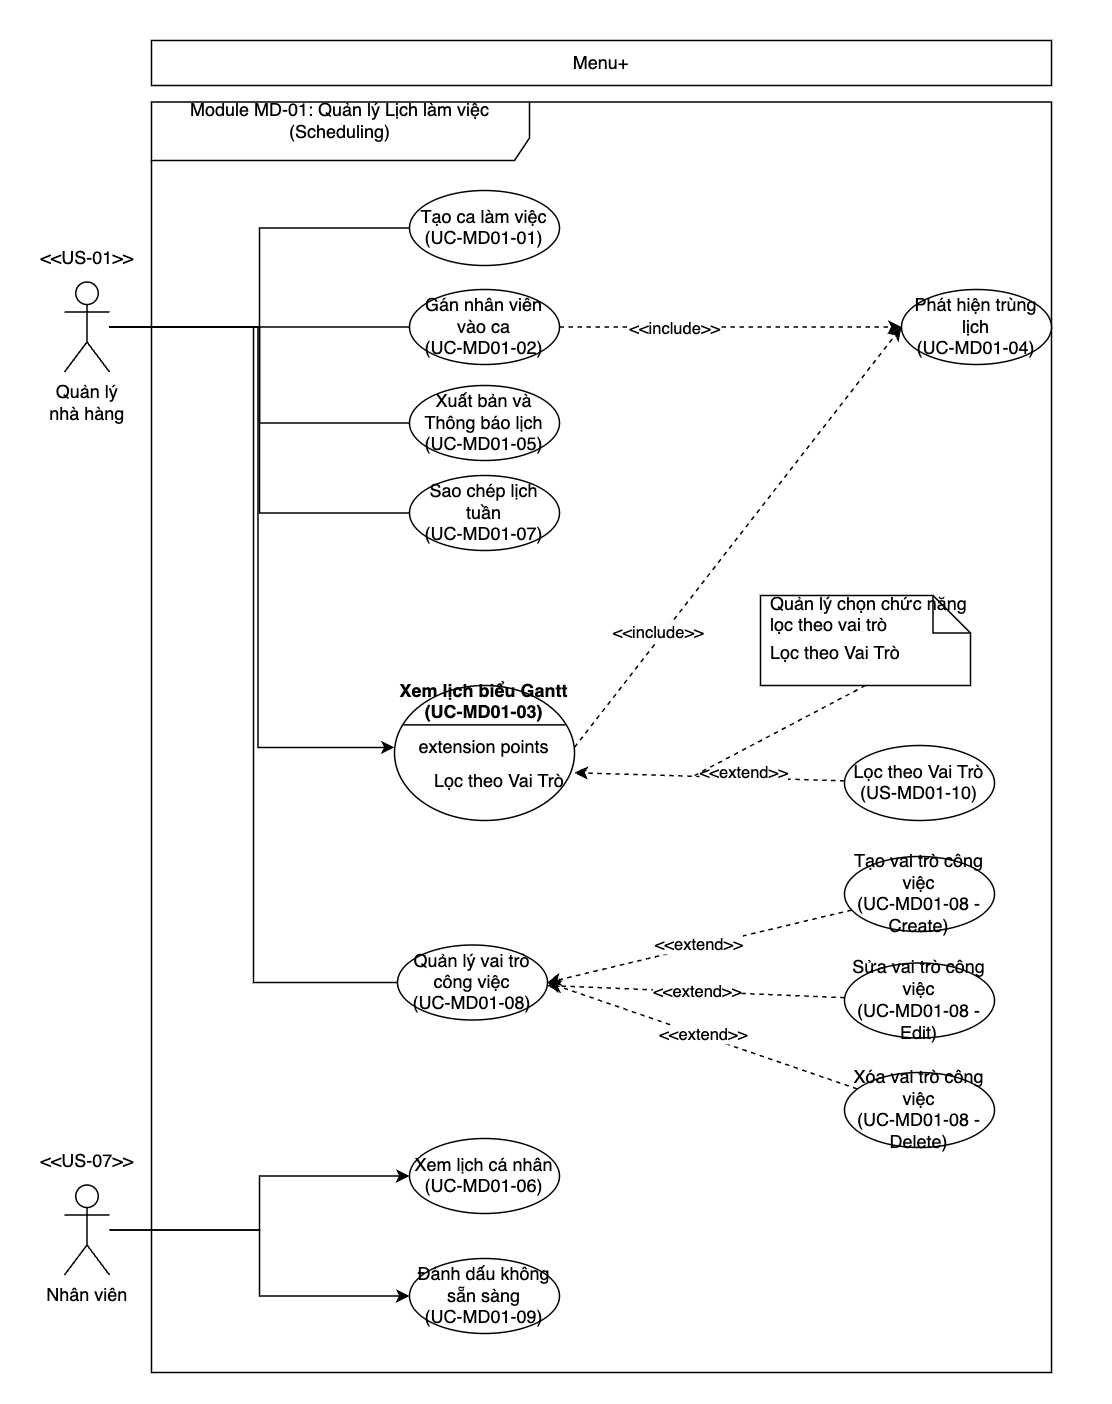
\includegraphics[width=15cm]{Sections/tong_quan/functional_spec/img/ucd01.png}

     \vspace{0.5cm}
    \caption{Use case diagram cho Module MD-01: Quản lý Lịch làm việc (Scheduling)}
\end{figure}

\subsubsubsection{FR-MD01-01: Tạo ca làm việc mới}

\begin{figure}[H]
	\centering
	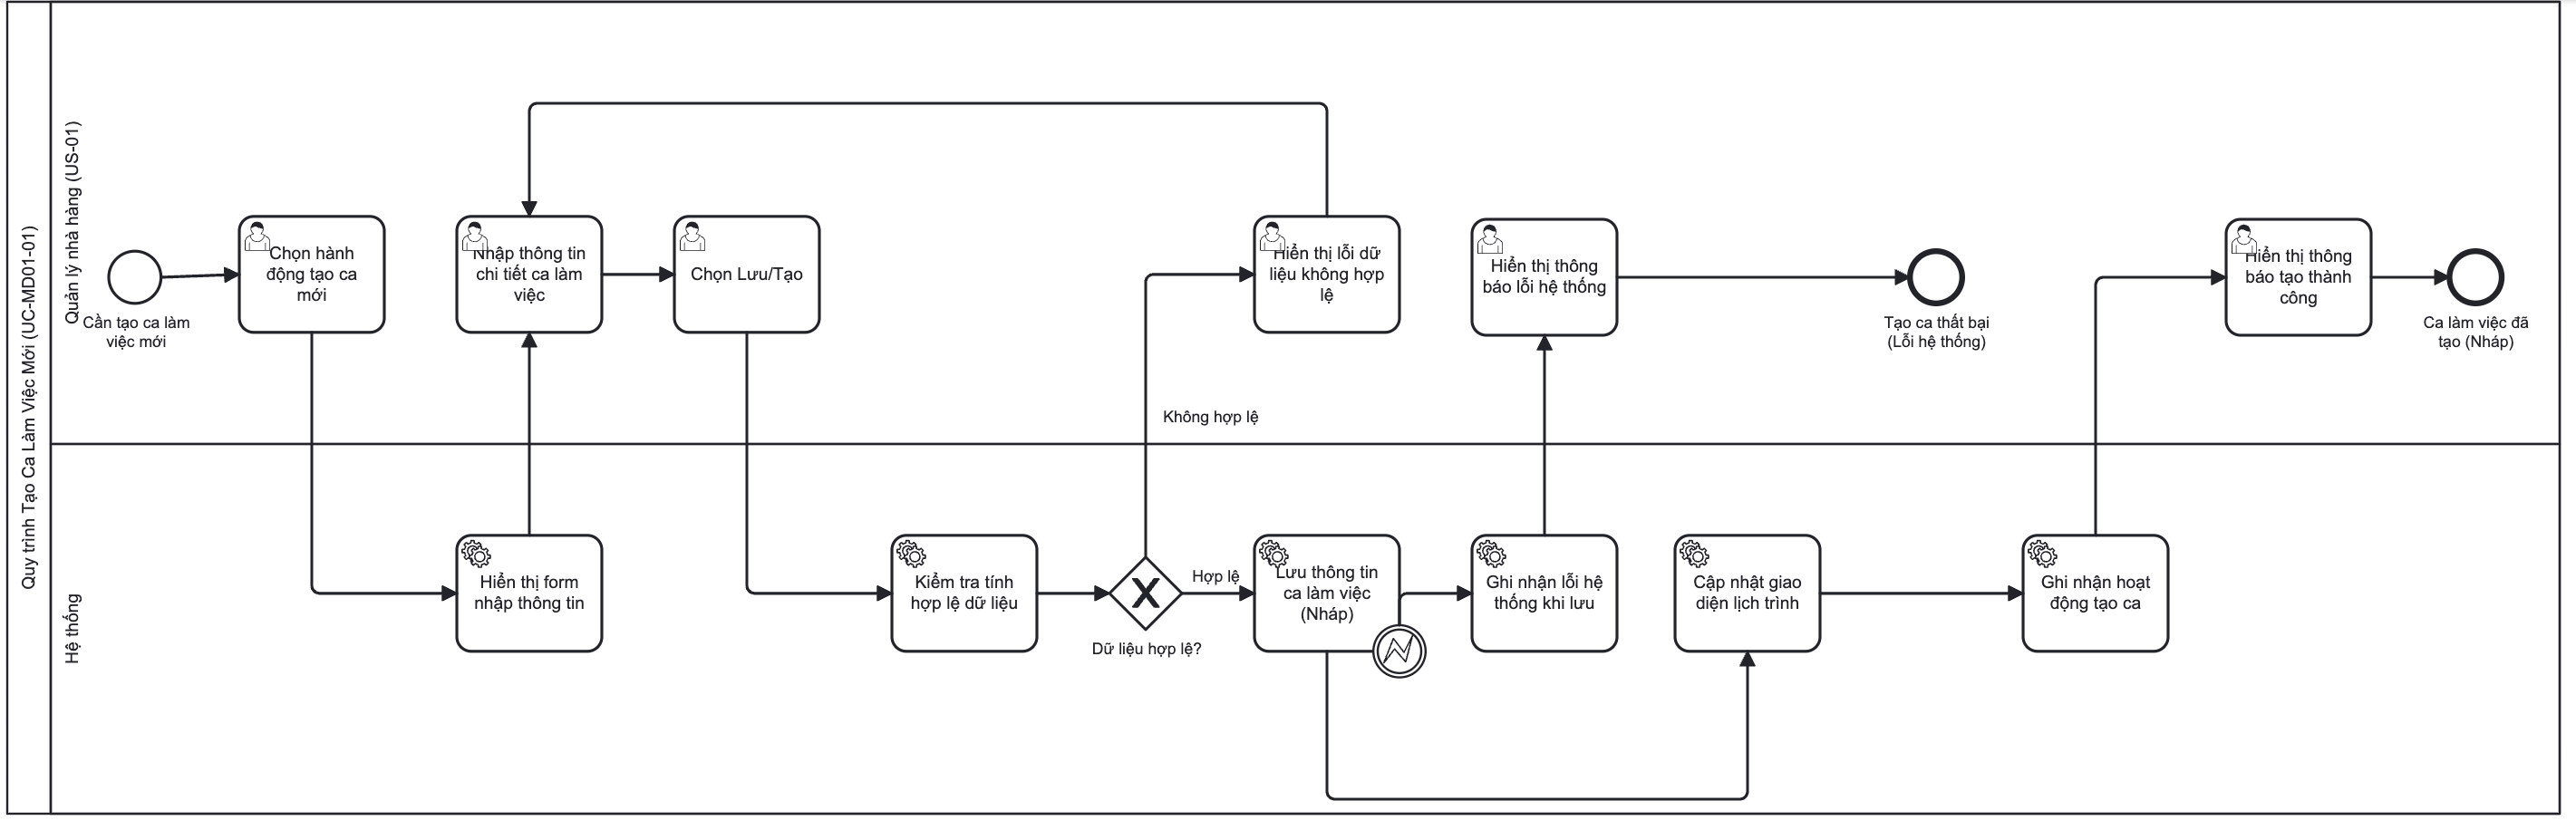
\includegraphics[width=15cm]{Sections/tong_quan/functional_spec/img/Screenshot 2025-04-30 at 20.11.53.png}

     \vspace{0.5cm}
    \caption{Quy trình Tạo ca làm việc mới (UC-MD-1-01)}
\end{figure}

\subsubsubsection{FR-MD01-02: Gán nhân viên vào ca làm việc}
\begin{figure}[H]
	\centering
	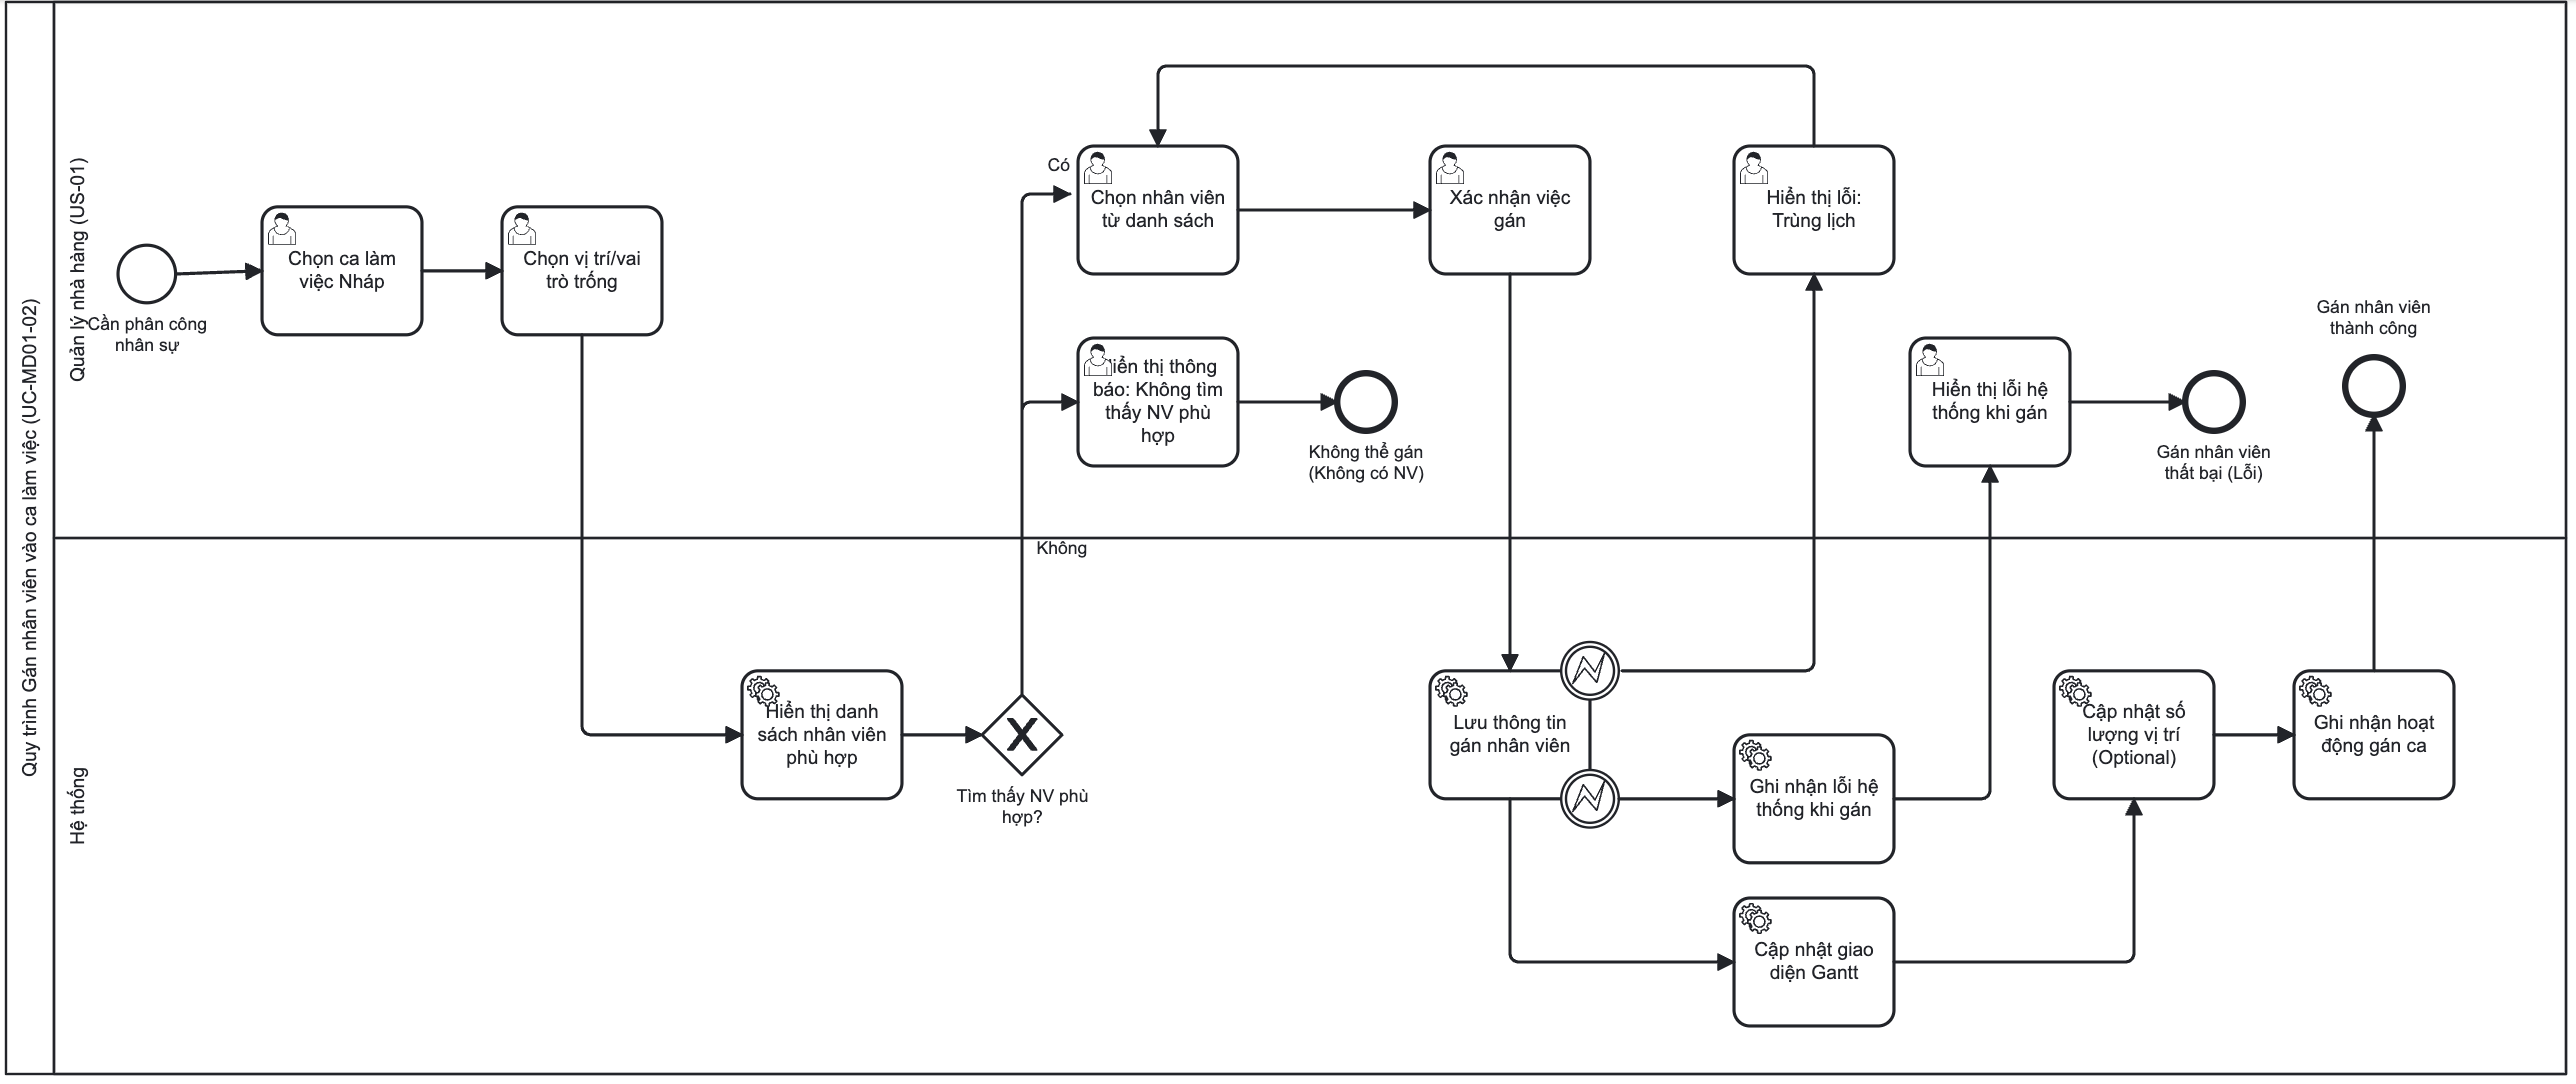
\includegraphics[width=15cm]{Sections/tong_quan/functional_spec/img/1.2.png}

     \vspace{0.5cm}
    \caption{Quy trình Gán nhân viên vào ca làm việc (UC-MD-1-02)}
\end{figure}


\subsubsubsection{FR-MD01-03: Xem lịch biểu Gantt}

\begin{figure}[H]
	\centering
	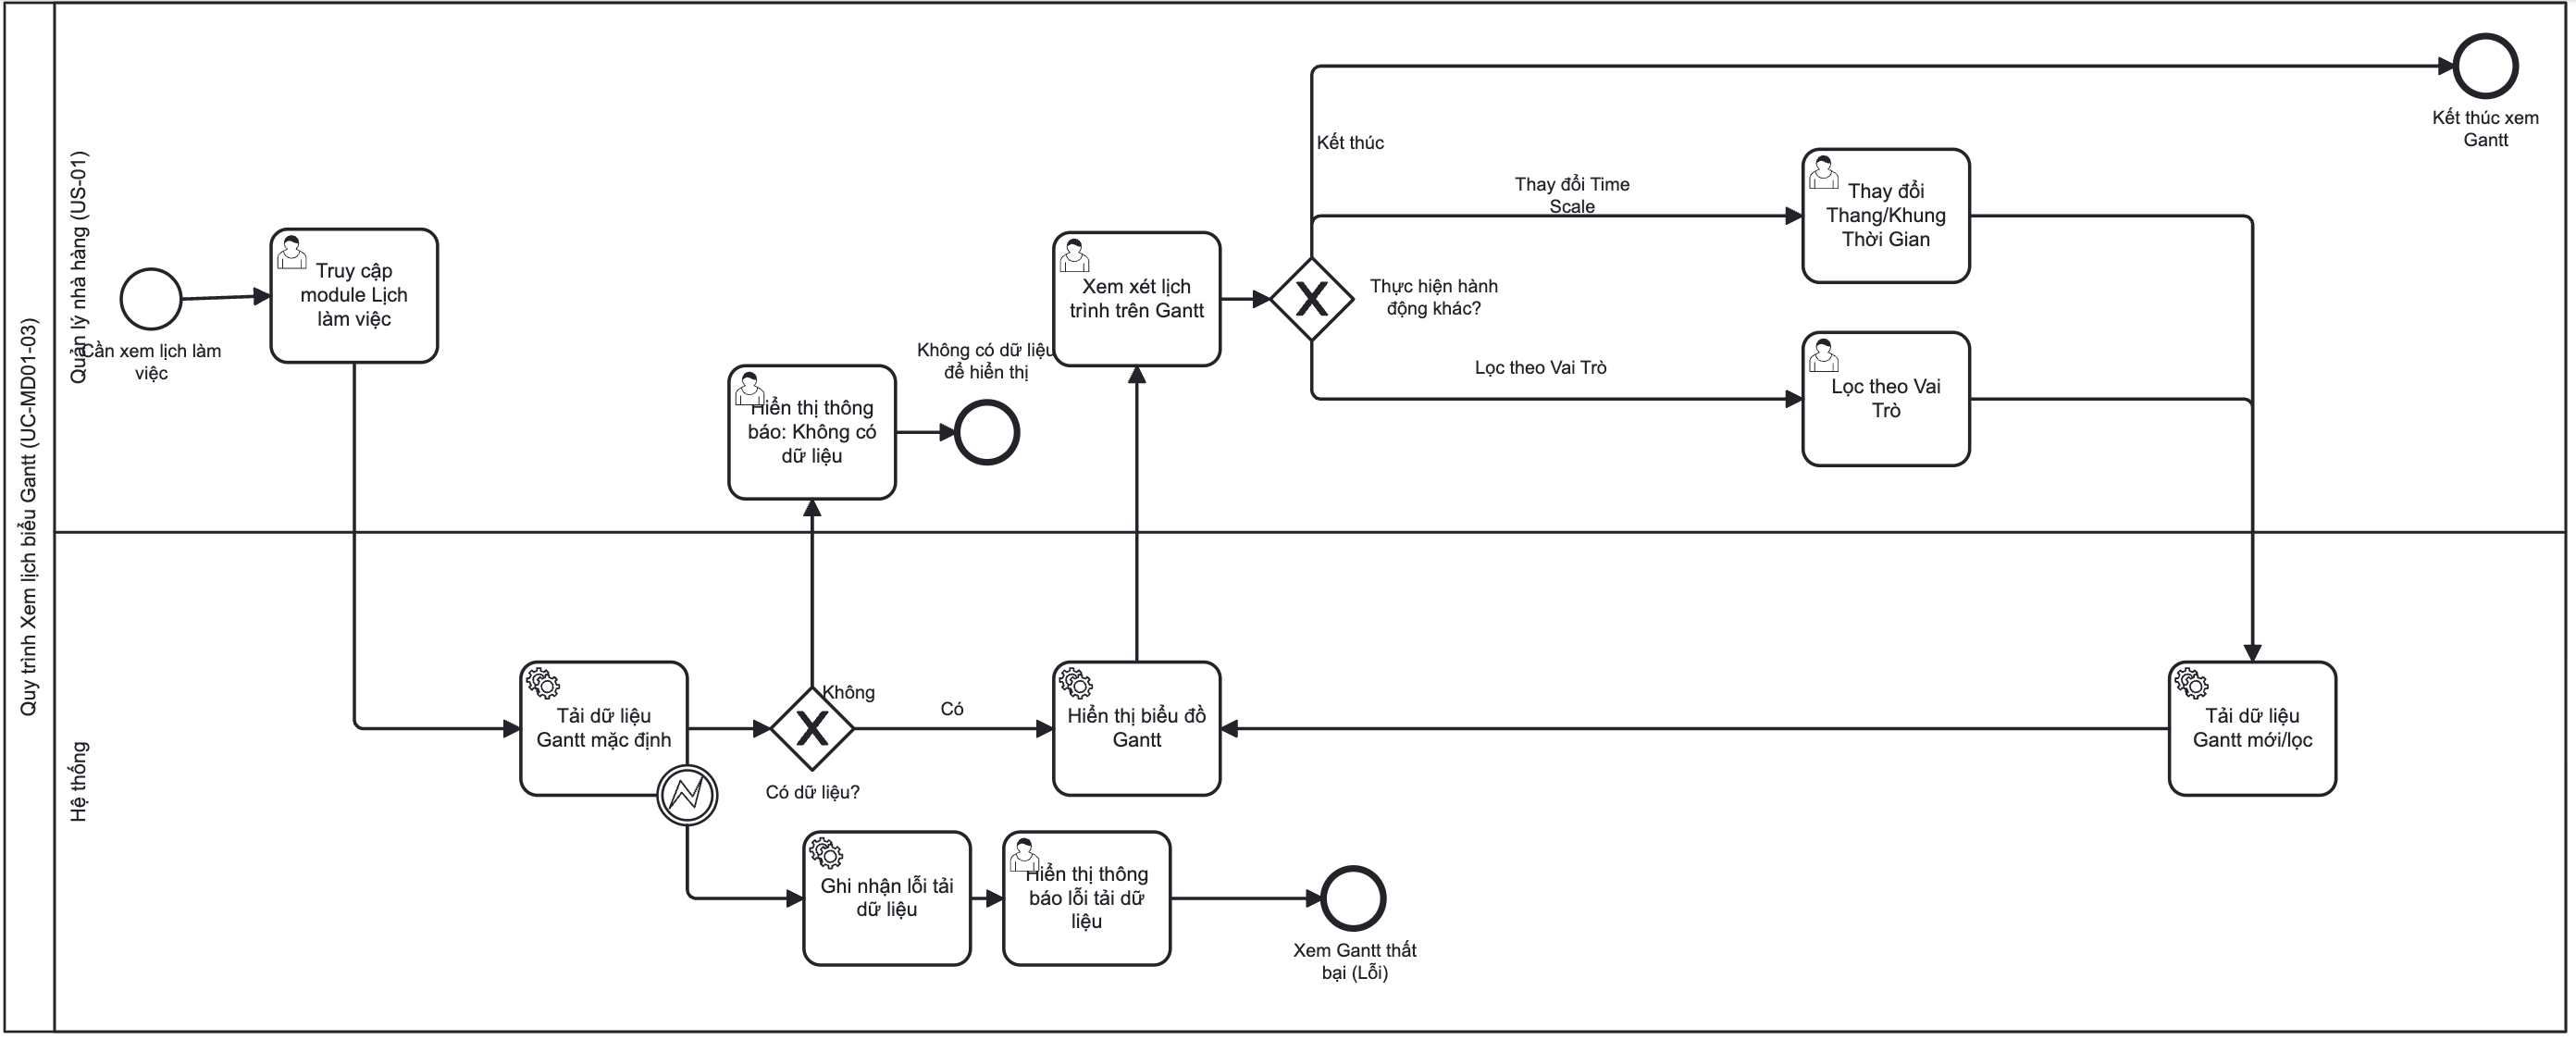
\includegraphics[width=15cm]{Sections/tong_quan/functional_spec/img/1.3.png}

     \vspace{0.5cm}
    \caption{Quy trình Xem lịch biểu Gantt (UC-MD-1-03)}
\end{figure}

\subsubsubsection{FR-MD01-05: Phát hiện và Cảnh báo Trùng lịch}

\begin{figure}[H]
	\centering
	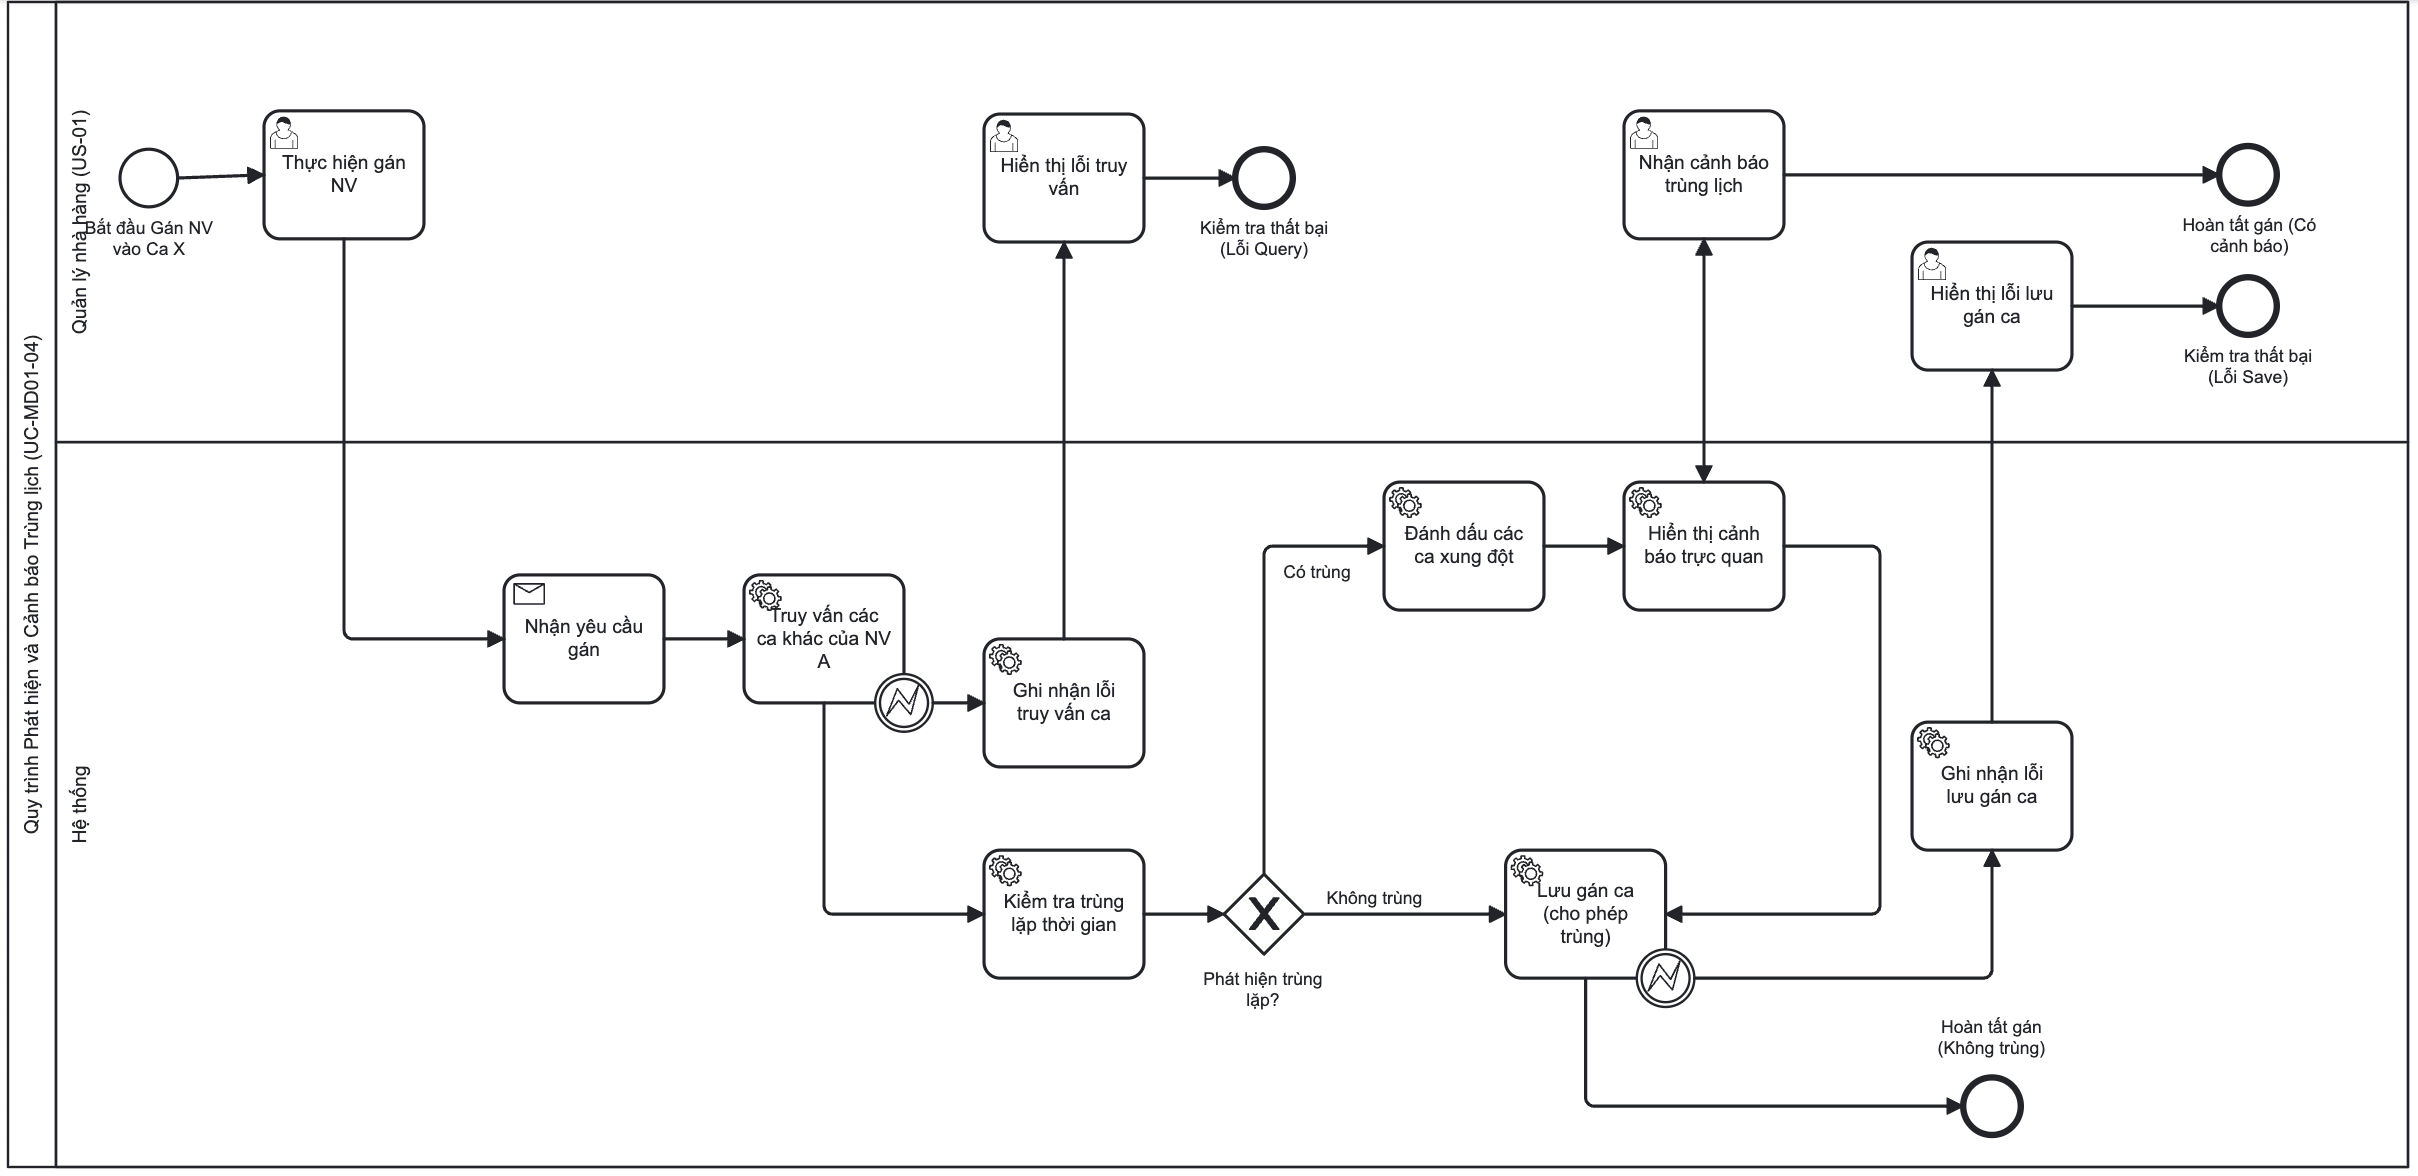
\includegraphics[width=15cm]{Sections/tong_quan/functional_spec/img/1.4.png}

     \vspace{0.5cm}
    \caption{Quy trình  Phát hiện và Cảnh báo Trùng lịch (UC-MD-1-04)}
\end{figure}

\subsubsubsection{FR-MD01-05: Xuất bản và Thông báo Lịch làm việc}


\subsubsubsection{FR-MD01-06: Xem lịch làm việc cá nhân}

\begin{figure}[H]
	\centering
	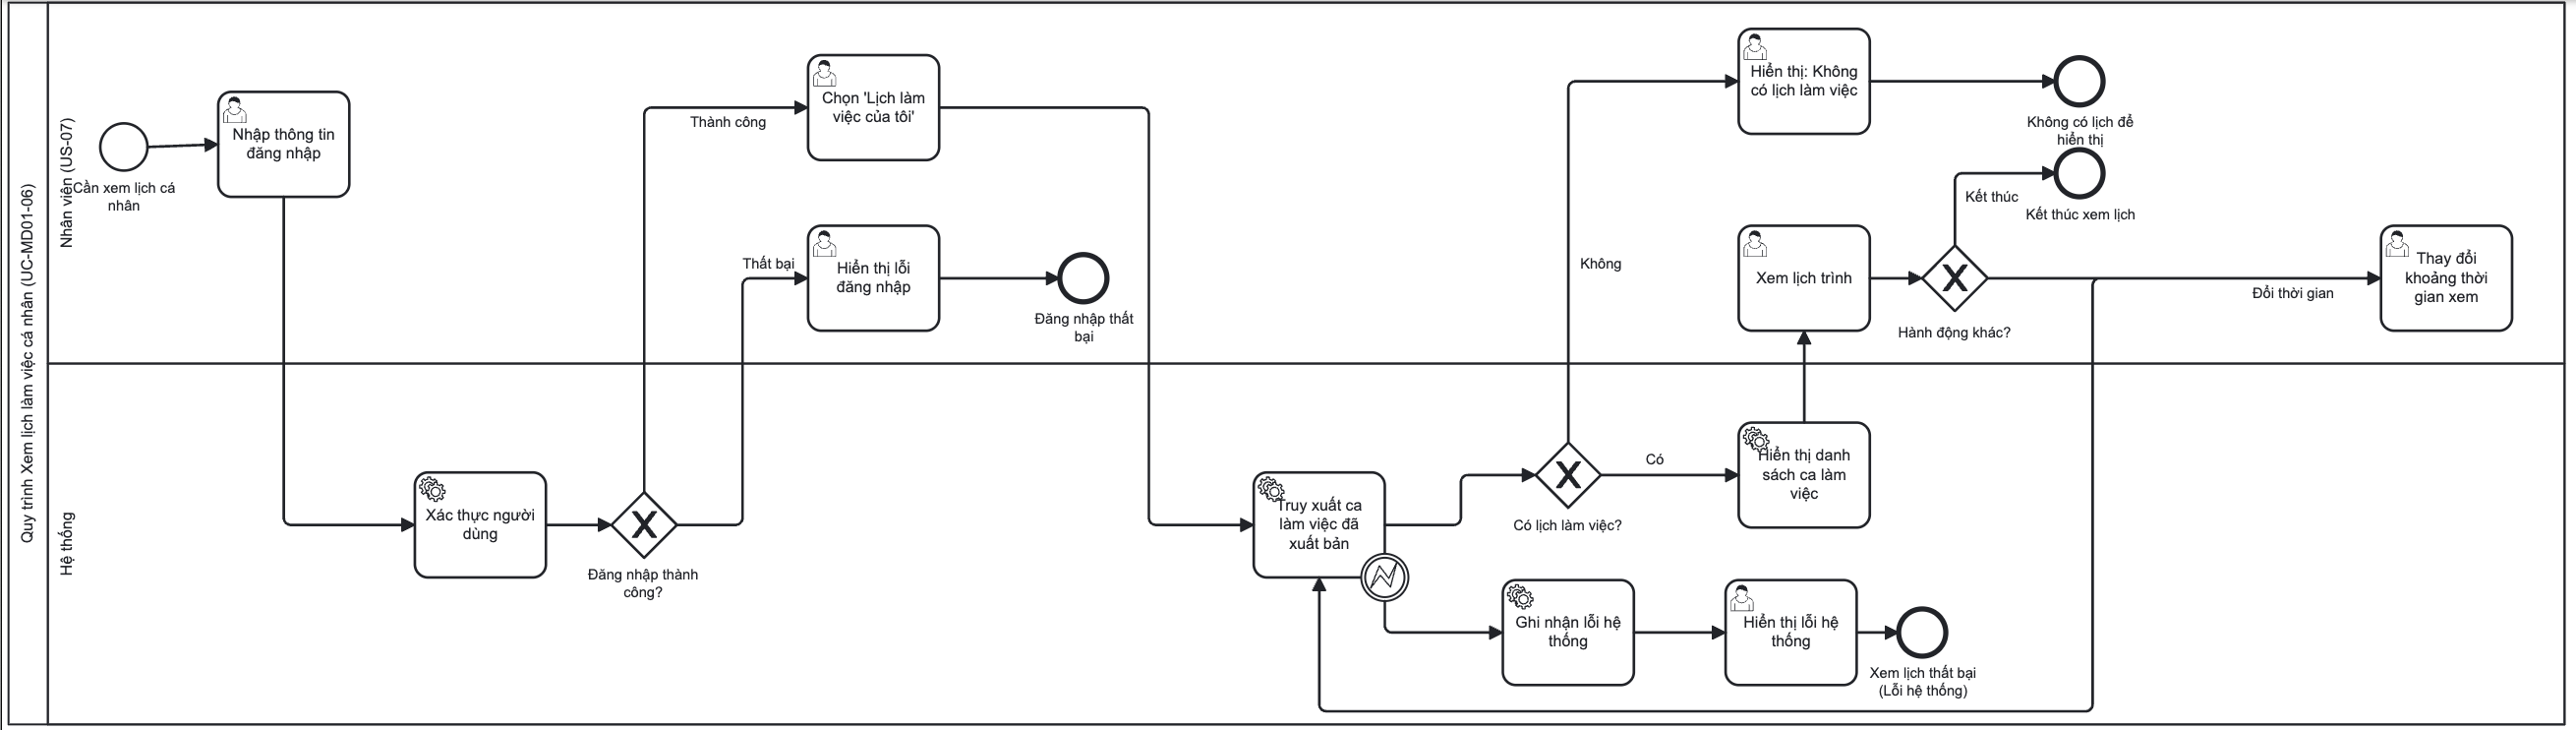
\includegraphics[width=15cm]{Sections/tong_quan/functional_spec/img/1.6.png}

     \vspace{0.5cm}
    \caption{Quy trình Xem lịch làm việc cá nhân (UC-MD-1-06)}
\end{figure}

\subsubsubsection{FR-MD01-07: Sao chép lịch tuần}

\begin{figure}[H]
	\centering
	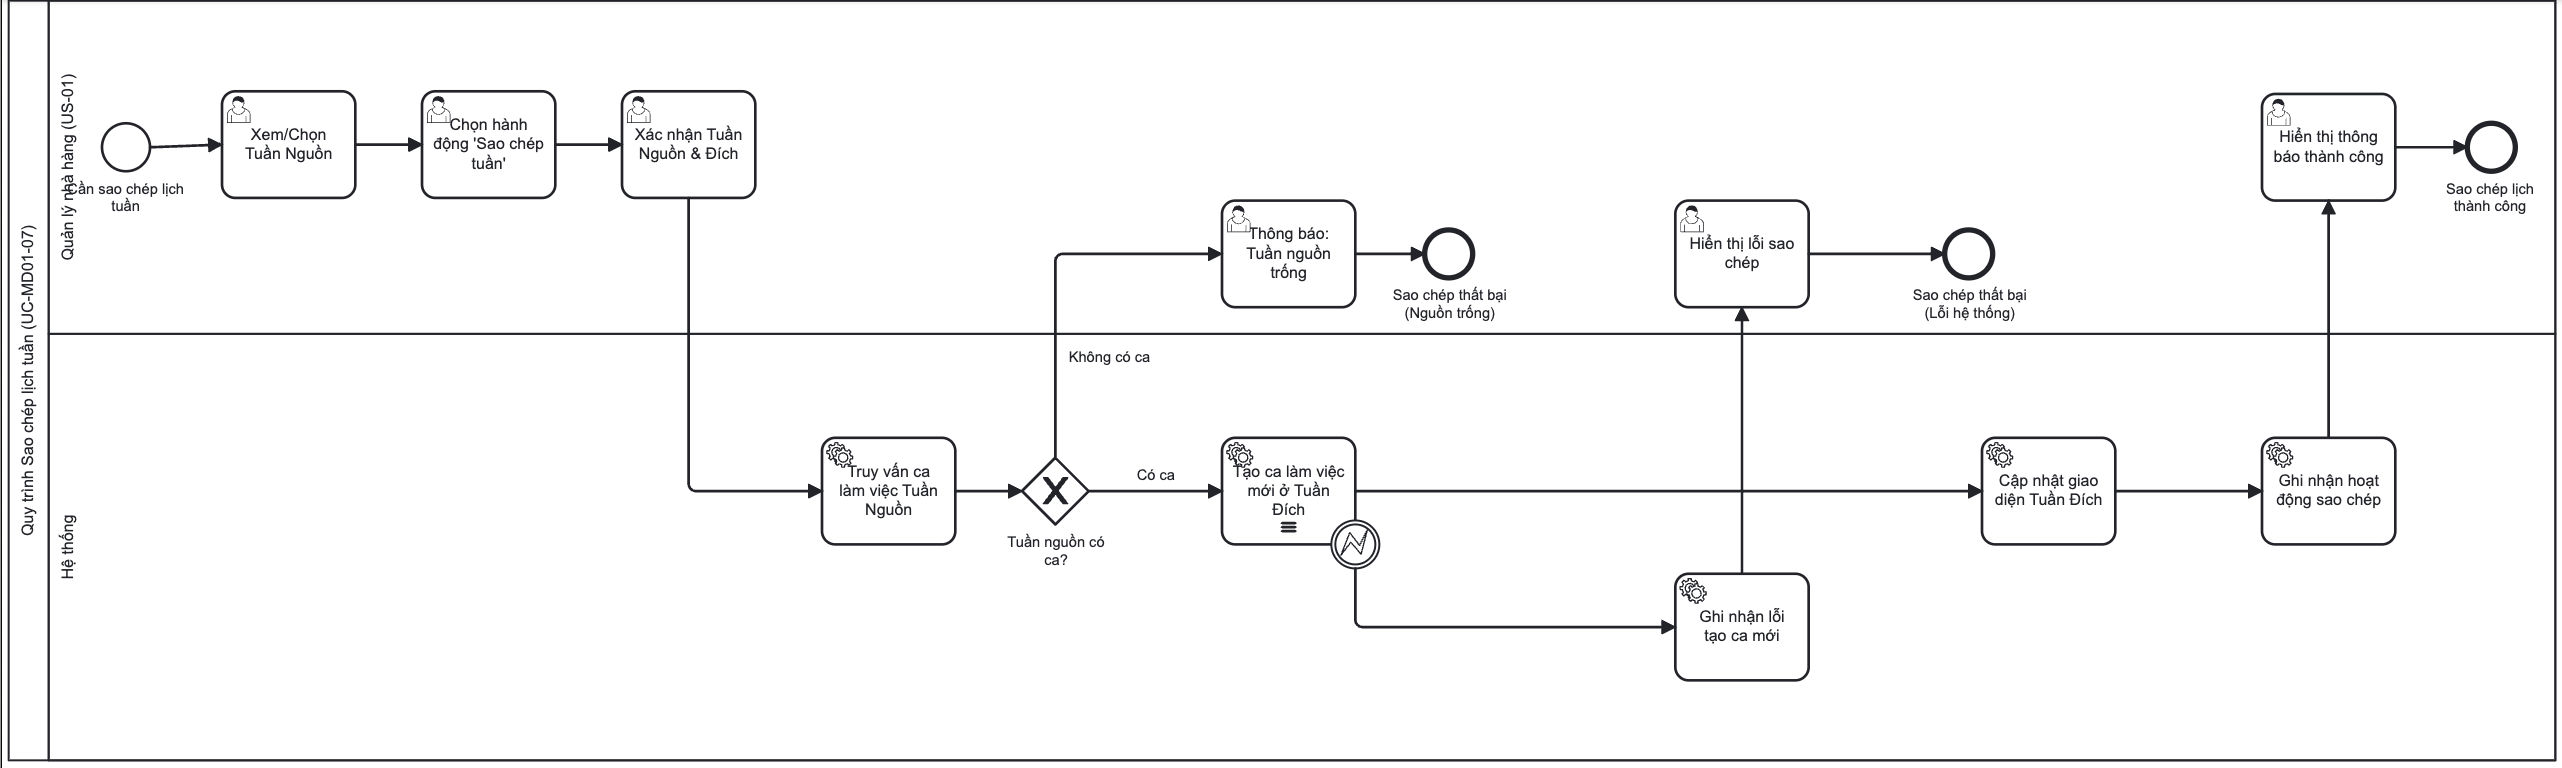
\includegraphics[width=15cm]{Sections/tong_quan/functional_spec/img/1.7.png}

     \vspace{0.5cm}
    \caption{Quy trình Sao chép lịch tuần (UC-MD-1-07)}
\end{figure}

\subsubsubsection{FR-MD01-08: Quản lý vai trò công việc}

\begin{figure}[H]
	\centering
	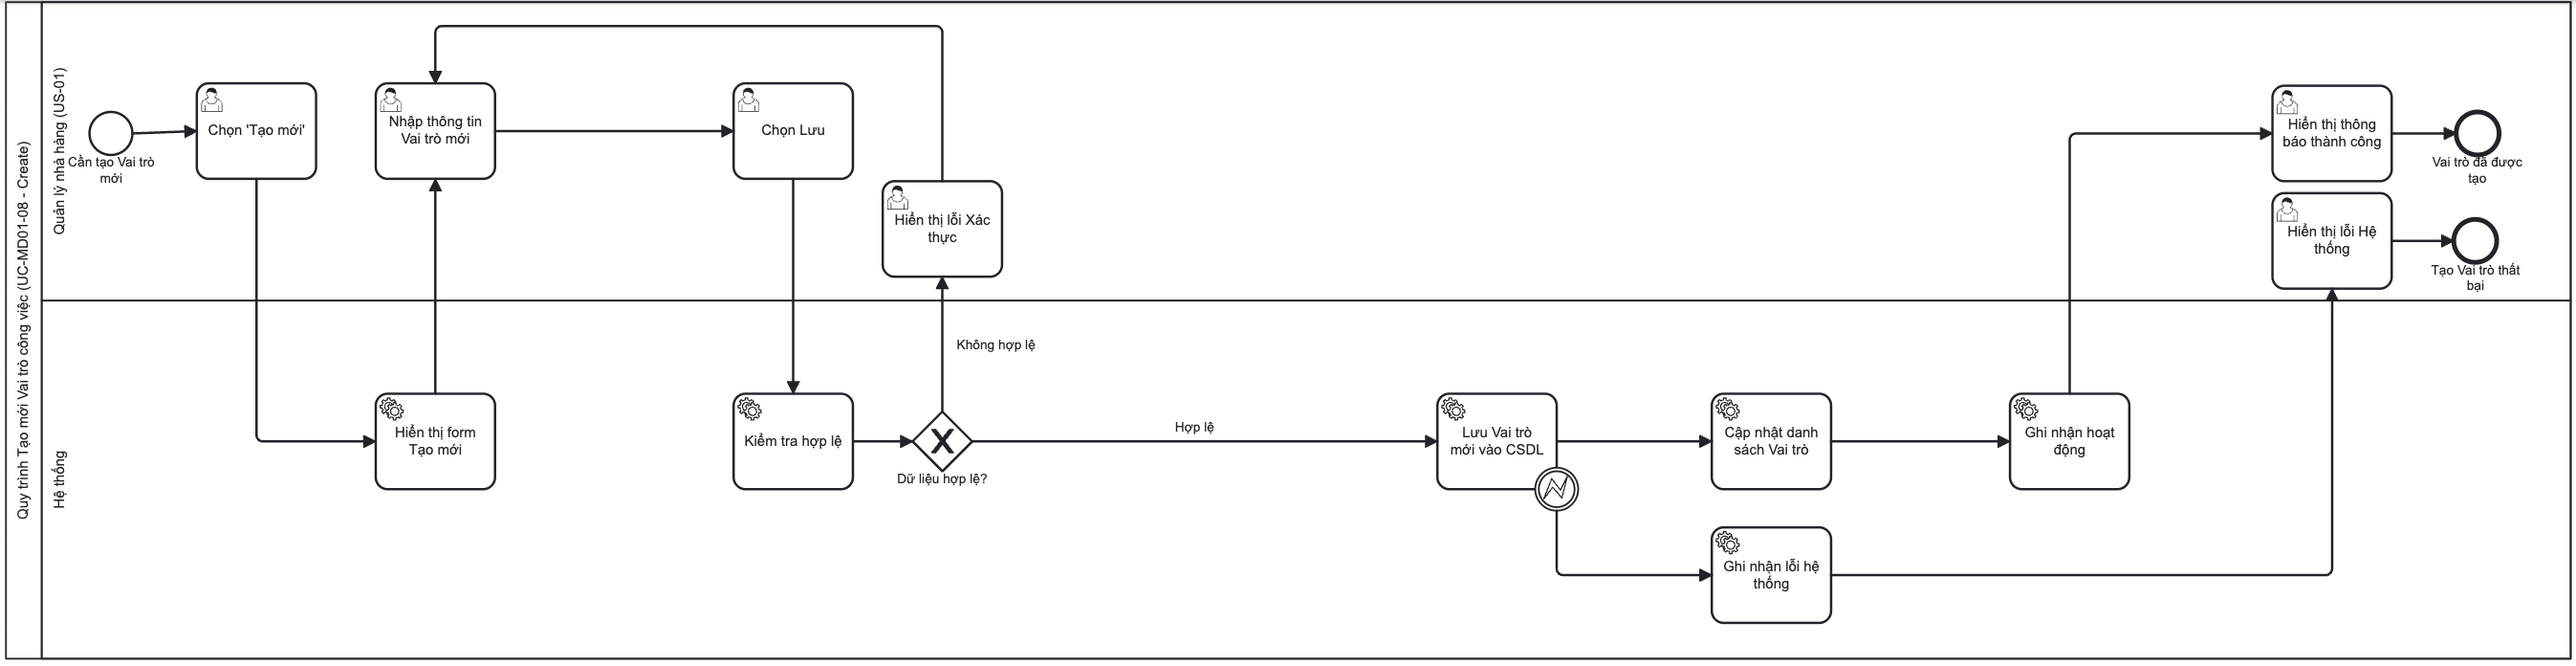
\includegraphics[width=15cm]{Sections/tong_quan/functional_spec/img/1.8.1.png}

     \vspace{0.5cm}
    \caption{Quy trình Tạo mới Vai trò công việc (UC-MD-1-08 - Create)}
\end{figure}
\begin{figure}[H]
	\centering
	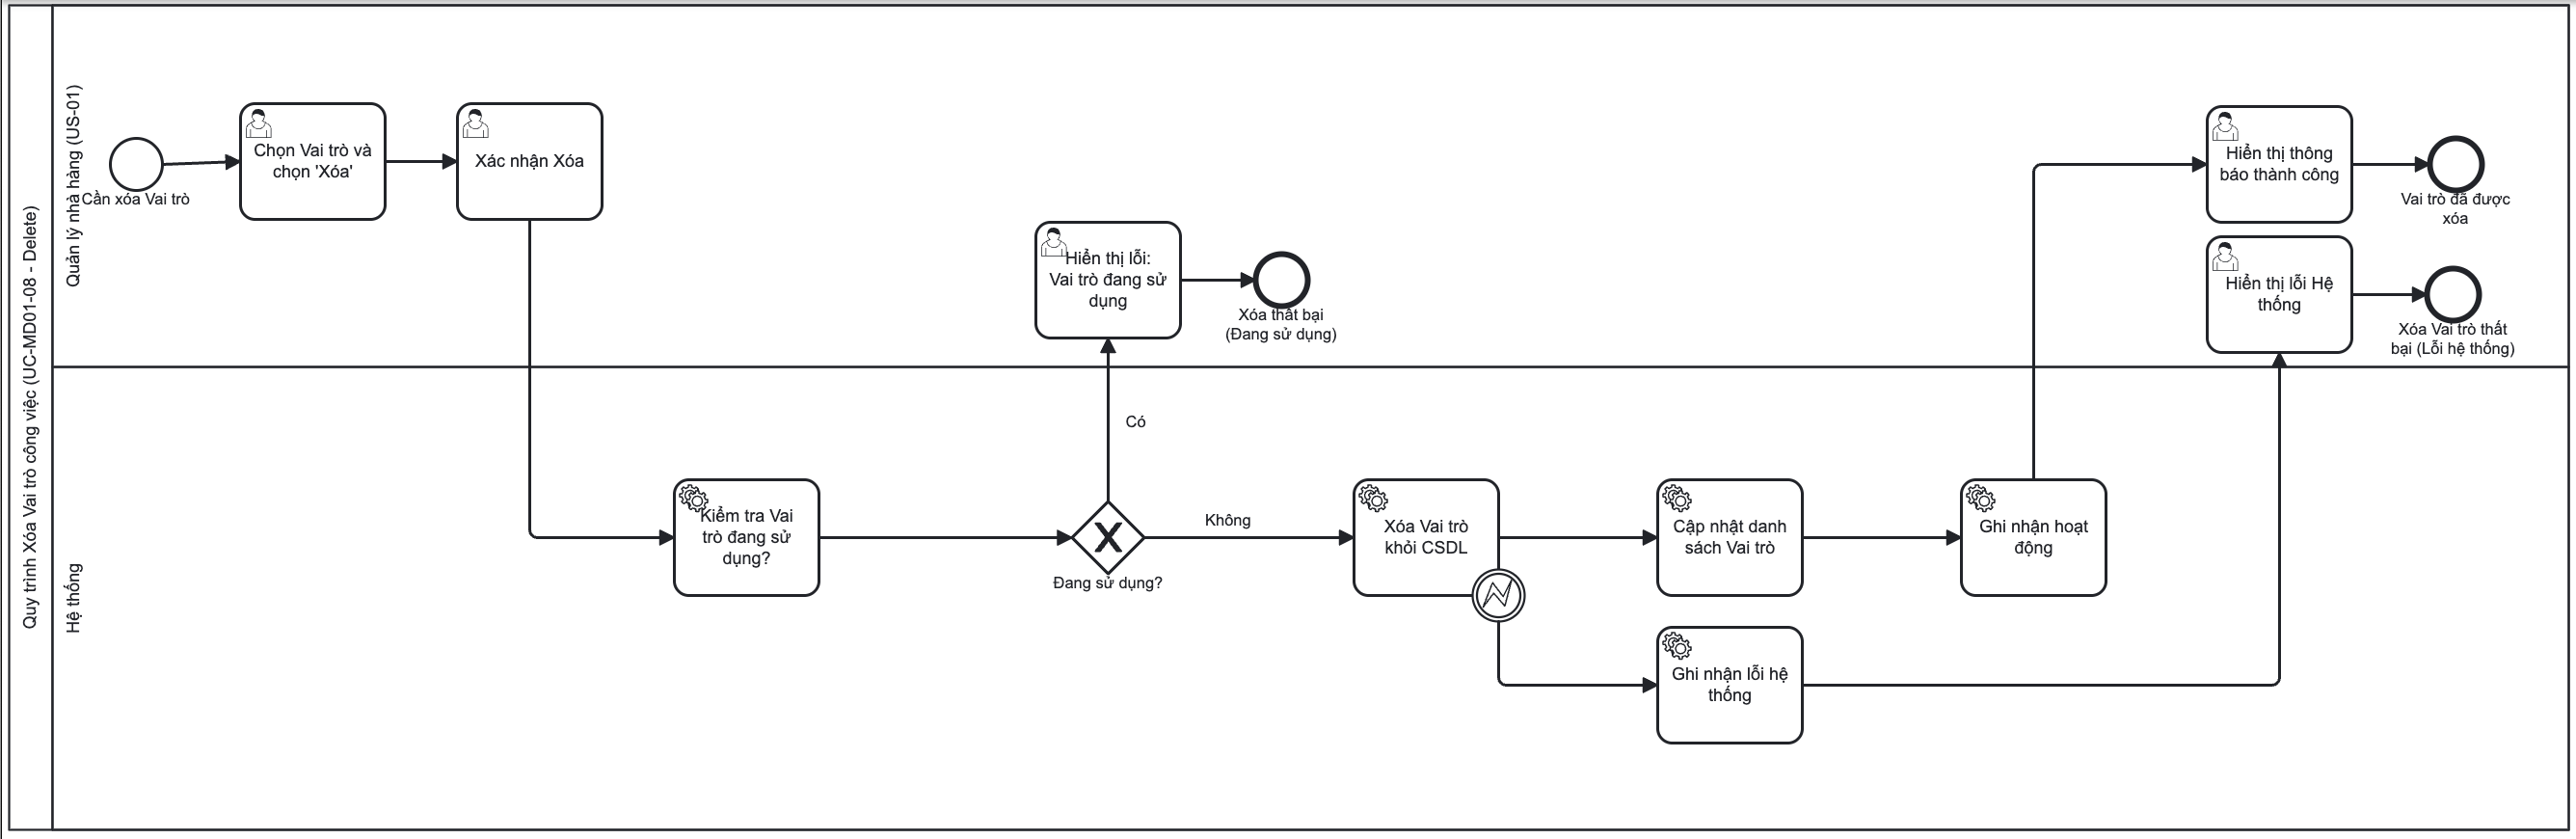
\includegraphics[width=15cm]{Sections/tong_quan/functional_spec/img/1.8.2.png}

     \vspace{0.5cm}
    \caption{Quy trình Xóa Vai trò công việc (UC-MD-1-08 - Delete)}
\end{figure}
\begin{figure}[H]
	\centering
	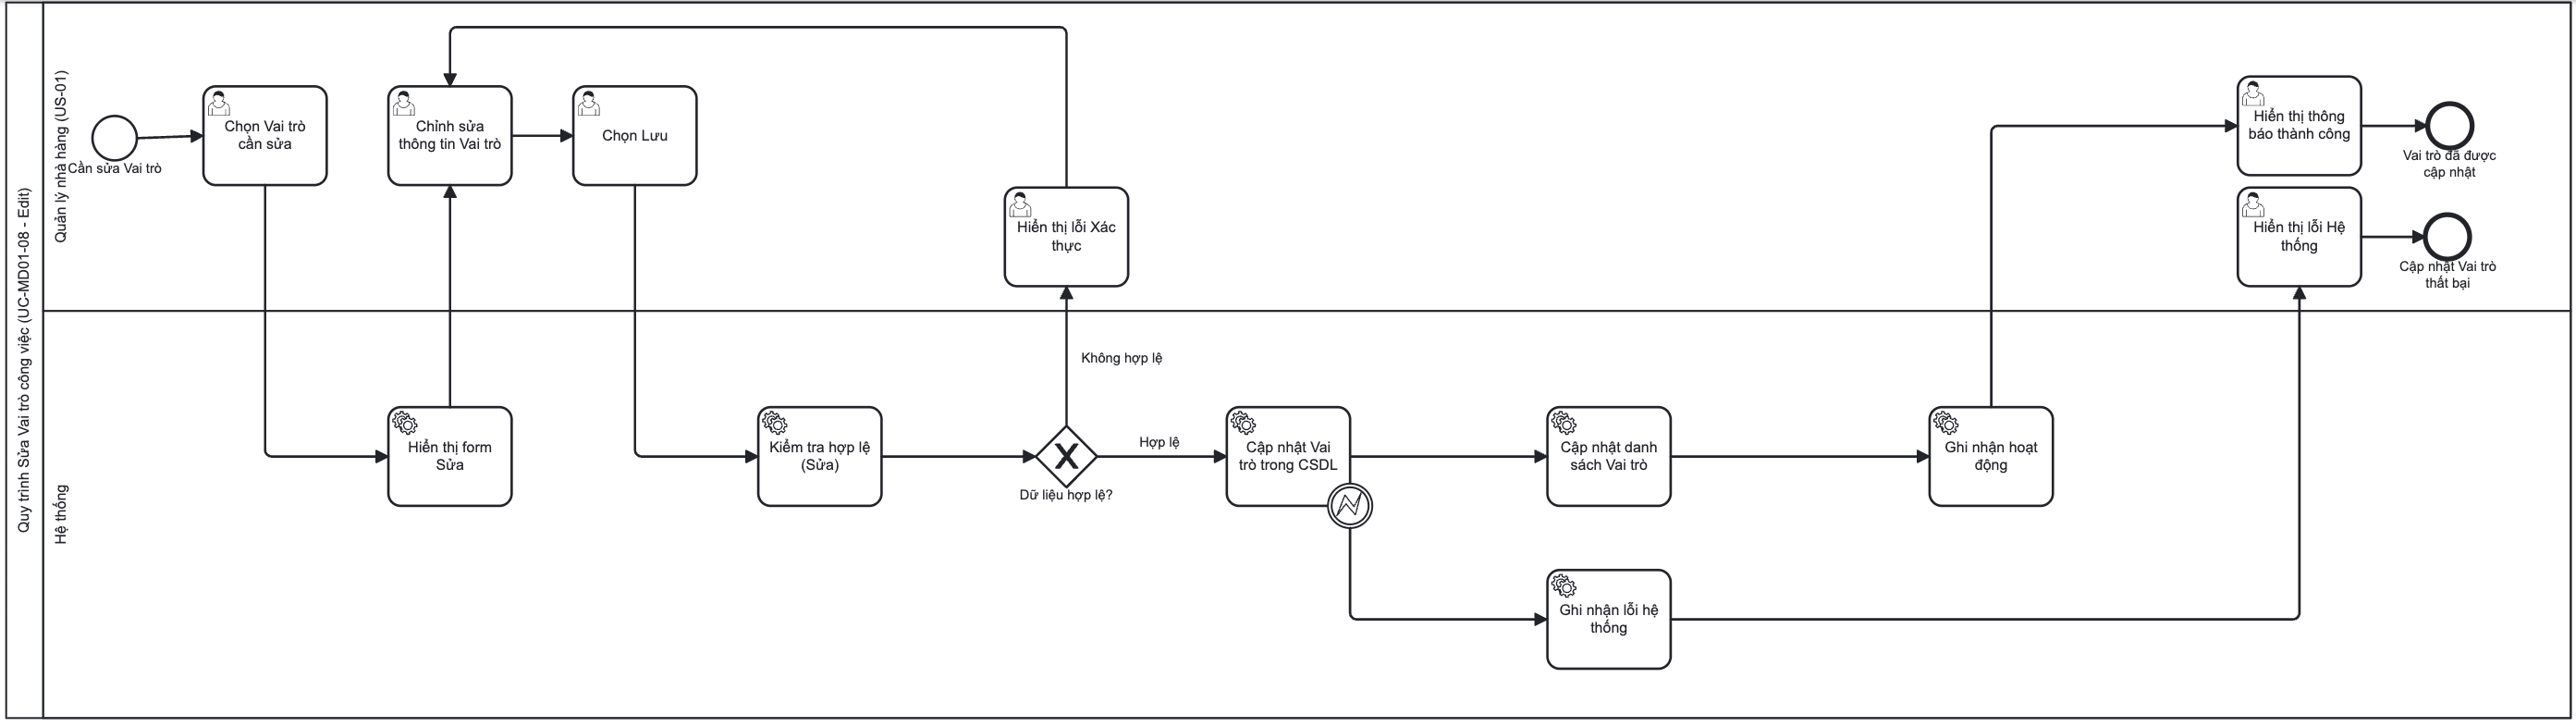
\includegraphics[width=15cm]{Sections/tong_quan/functional_spec/img/1.8.3.png}

     \vspace{0.5cm}
    \caption{Quy trình Sửa Vai trò công việc (UC-MD-1-08 - Edit)}
\end{figure}

\subsubsubsection{FR-MD01-09: Đánh dấu không sẵn sàng làm việc}

\begin{figure}[H]
	\centering
	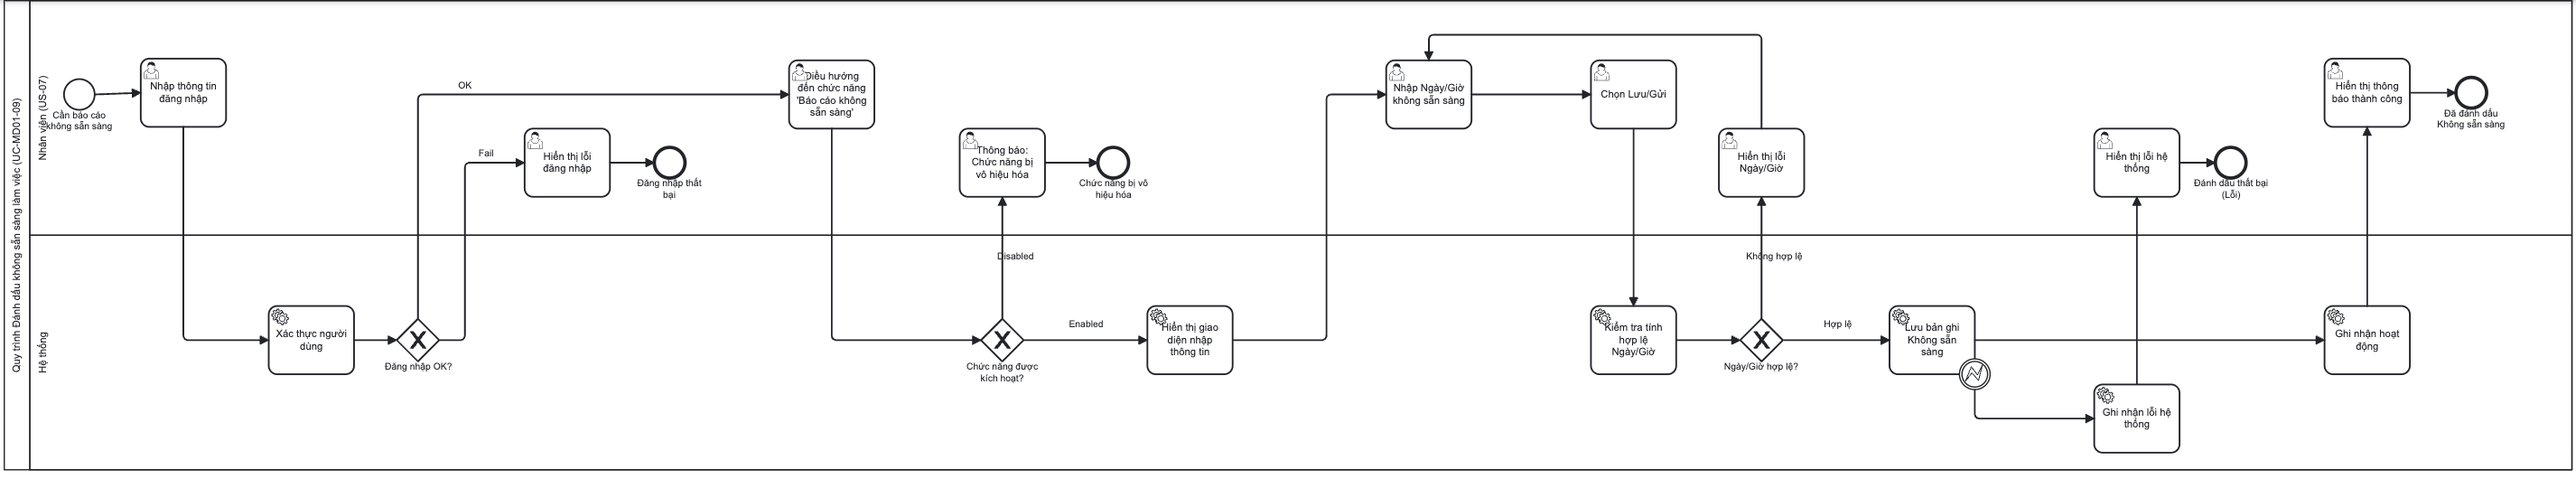
\includegraphics[width=15cm]{Sections/tong_quan/functional_spec/img/1.9.png}

     \vspace{0.5cm}
    \caption{Quy trình Đánh dấu không sẵn sàng làm việc (UC-MD-1-09)}
\end{figure}

\subsubsubsection{Use Case UC-MD01-10: Xem lịch theo vai trò}

\subsubsubsection{MVP (Minimum viable product) và Screen Flow}

\begin{figure}[H]
	\centering
	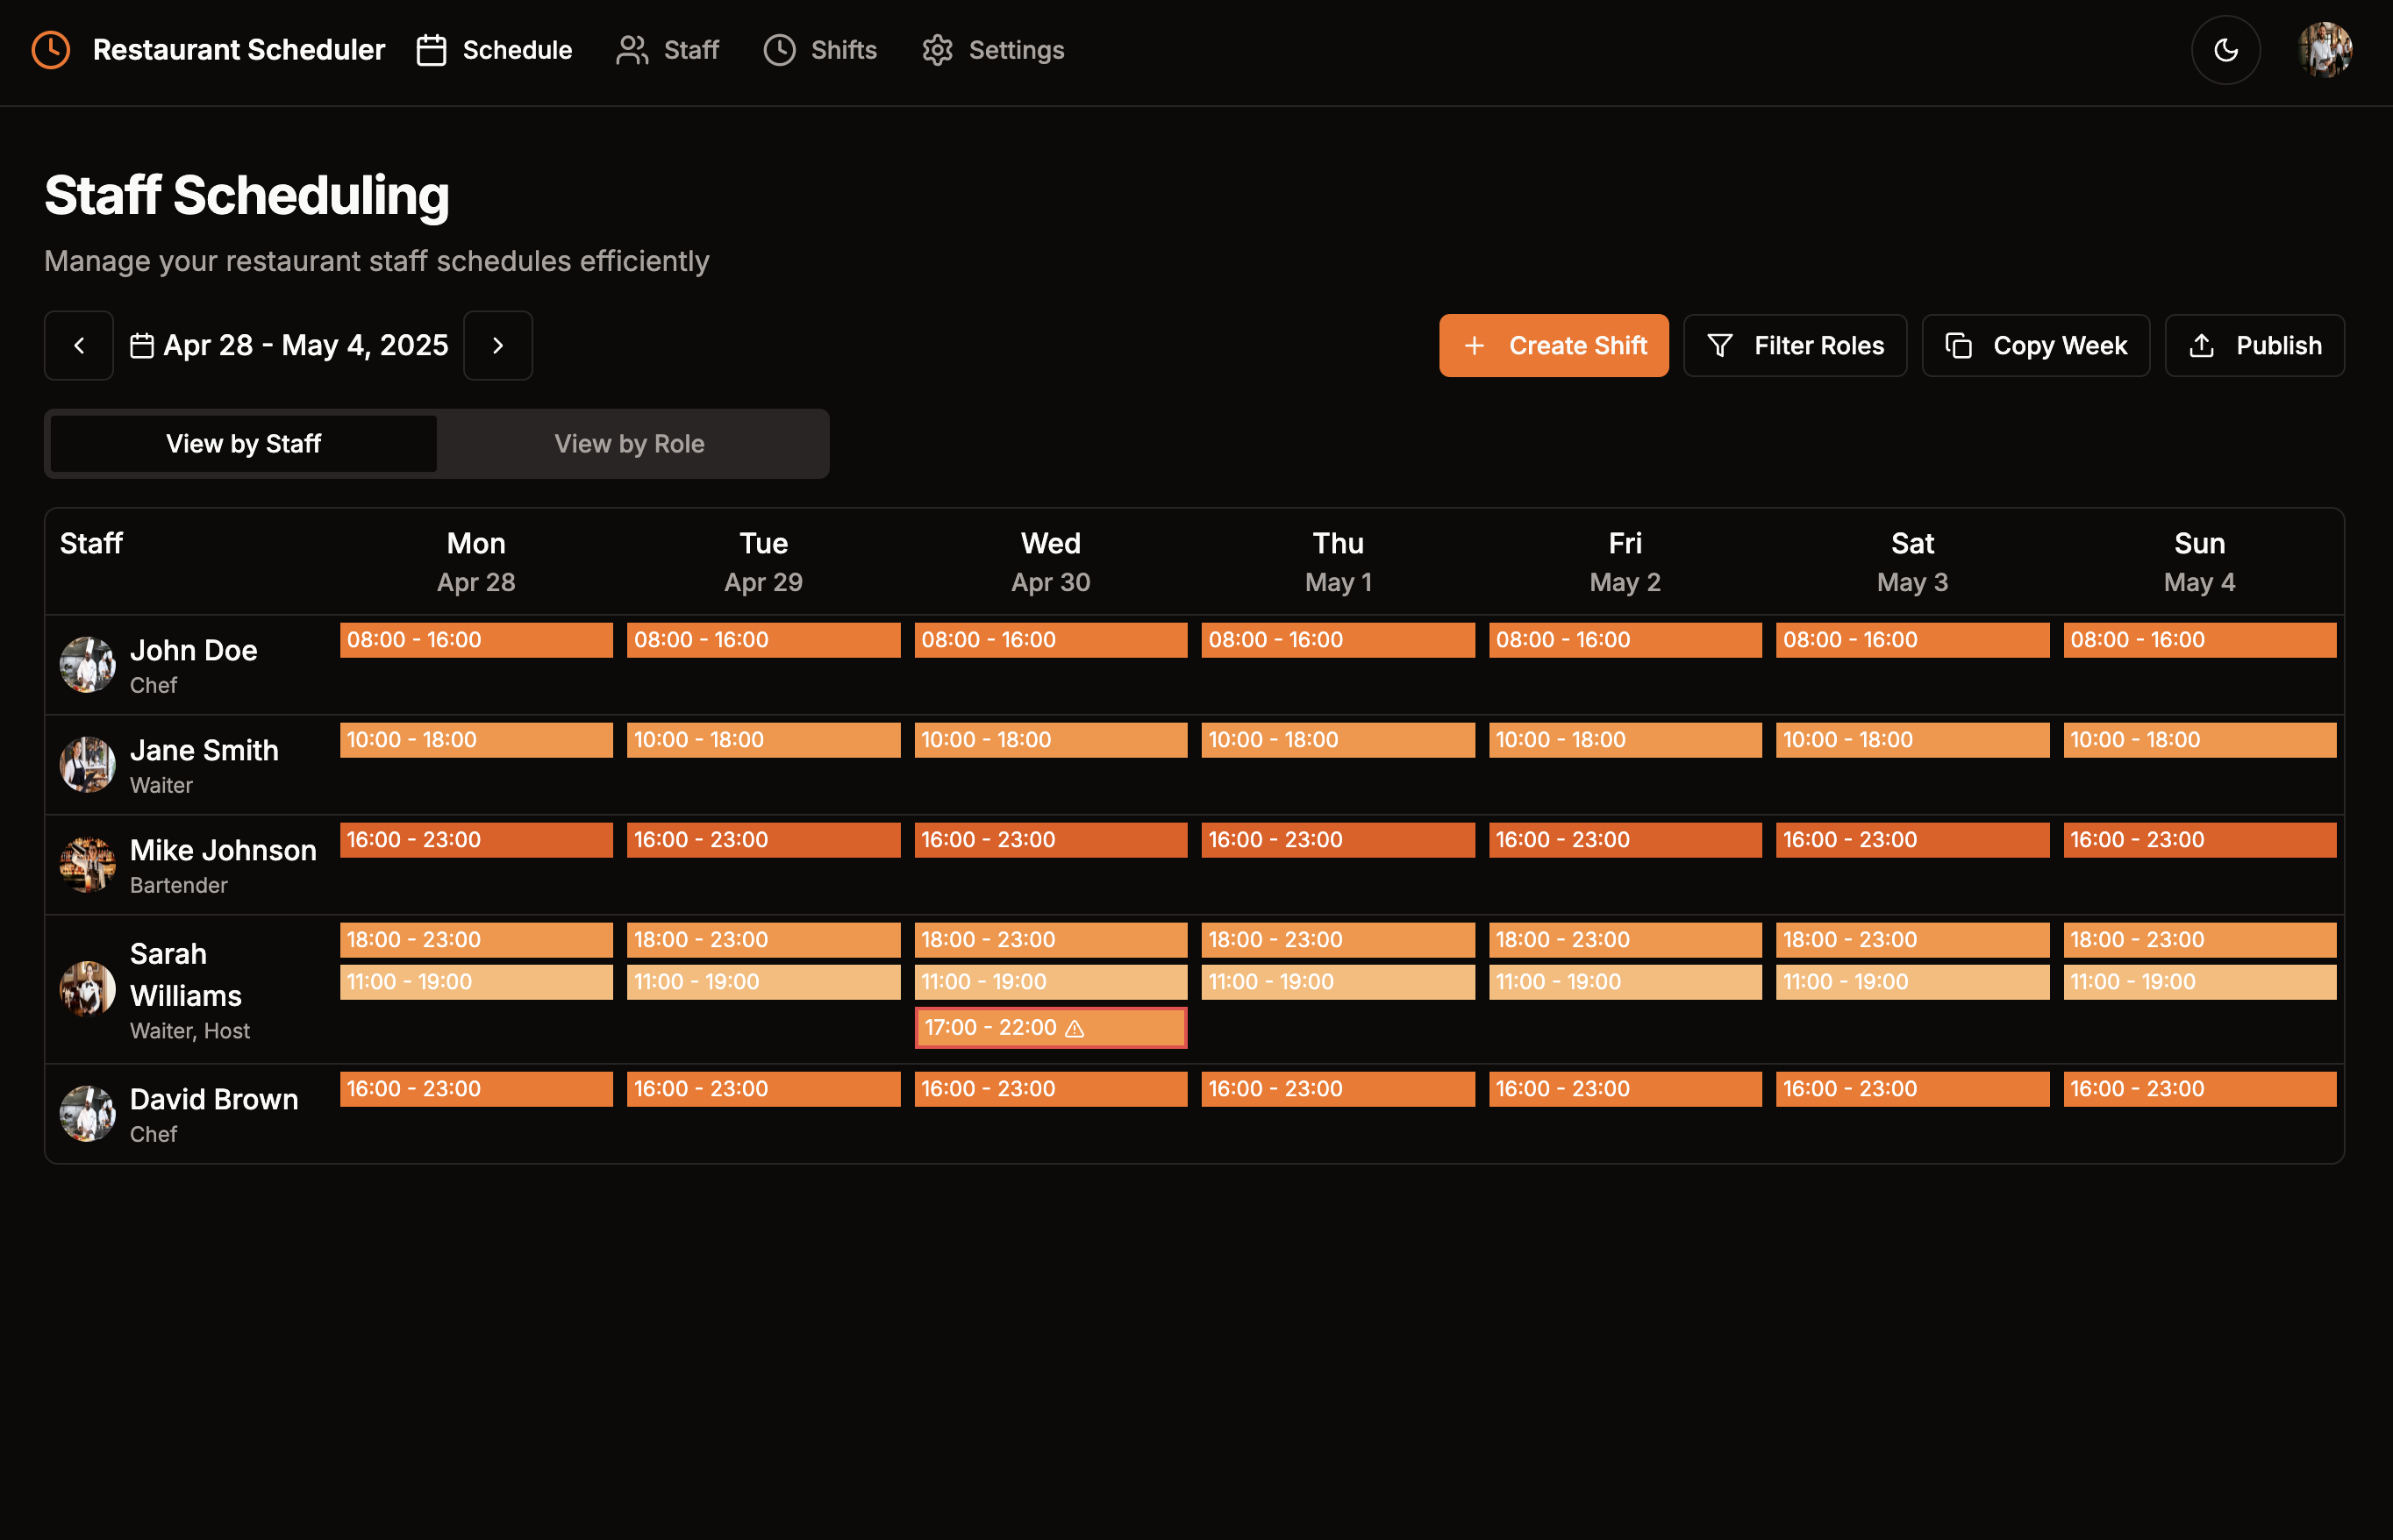
\includegraphics[width=15cm]{Sections/tong_quan/functional_spec/img/proto1.1.png}

     \vspace{0.5cm}
    \caption{Trang Dashboard (1)}
\end{figure}
\begin{figure}[H]
	\centering
	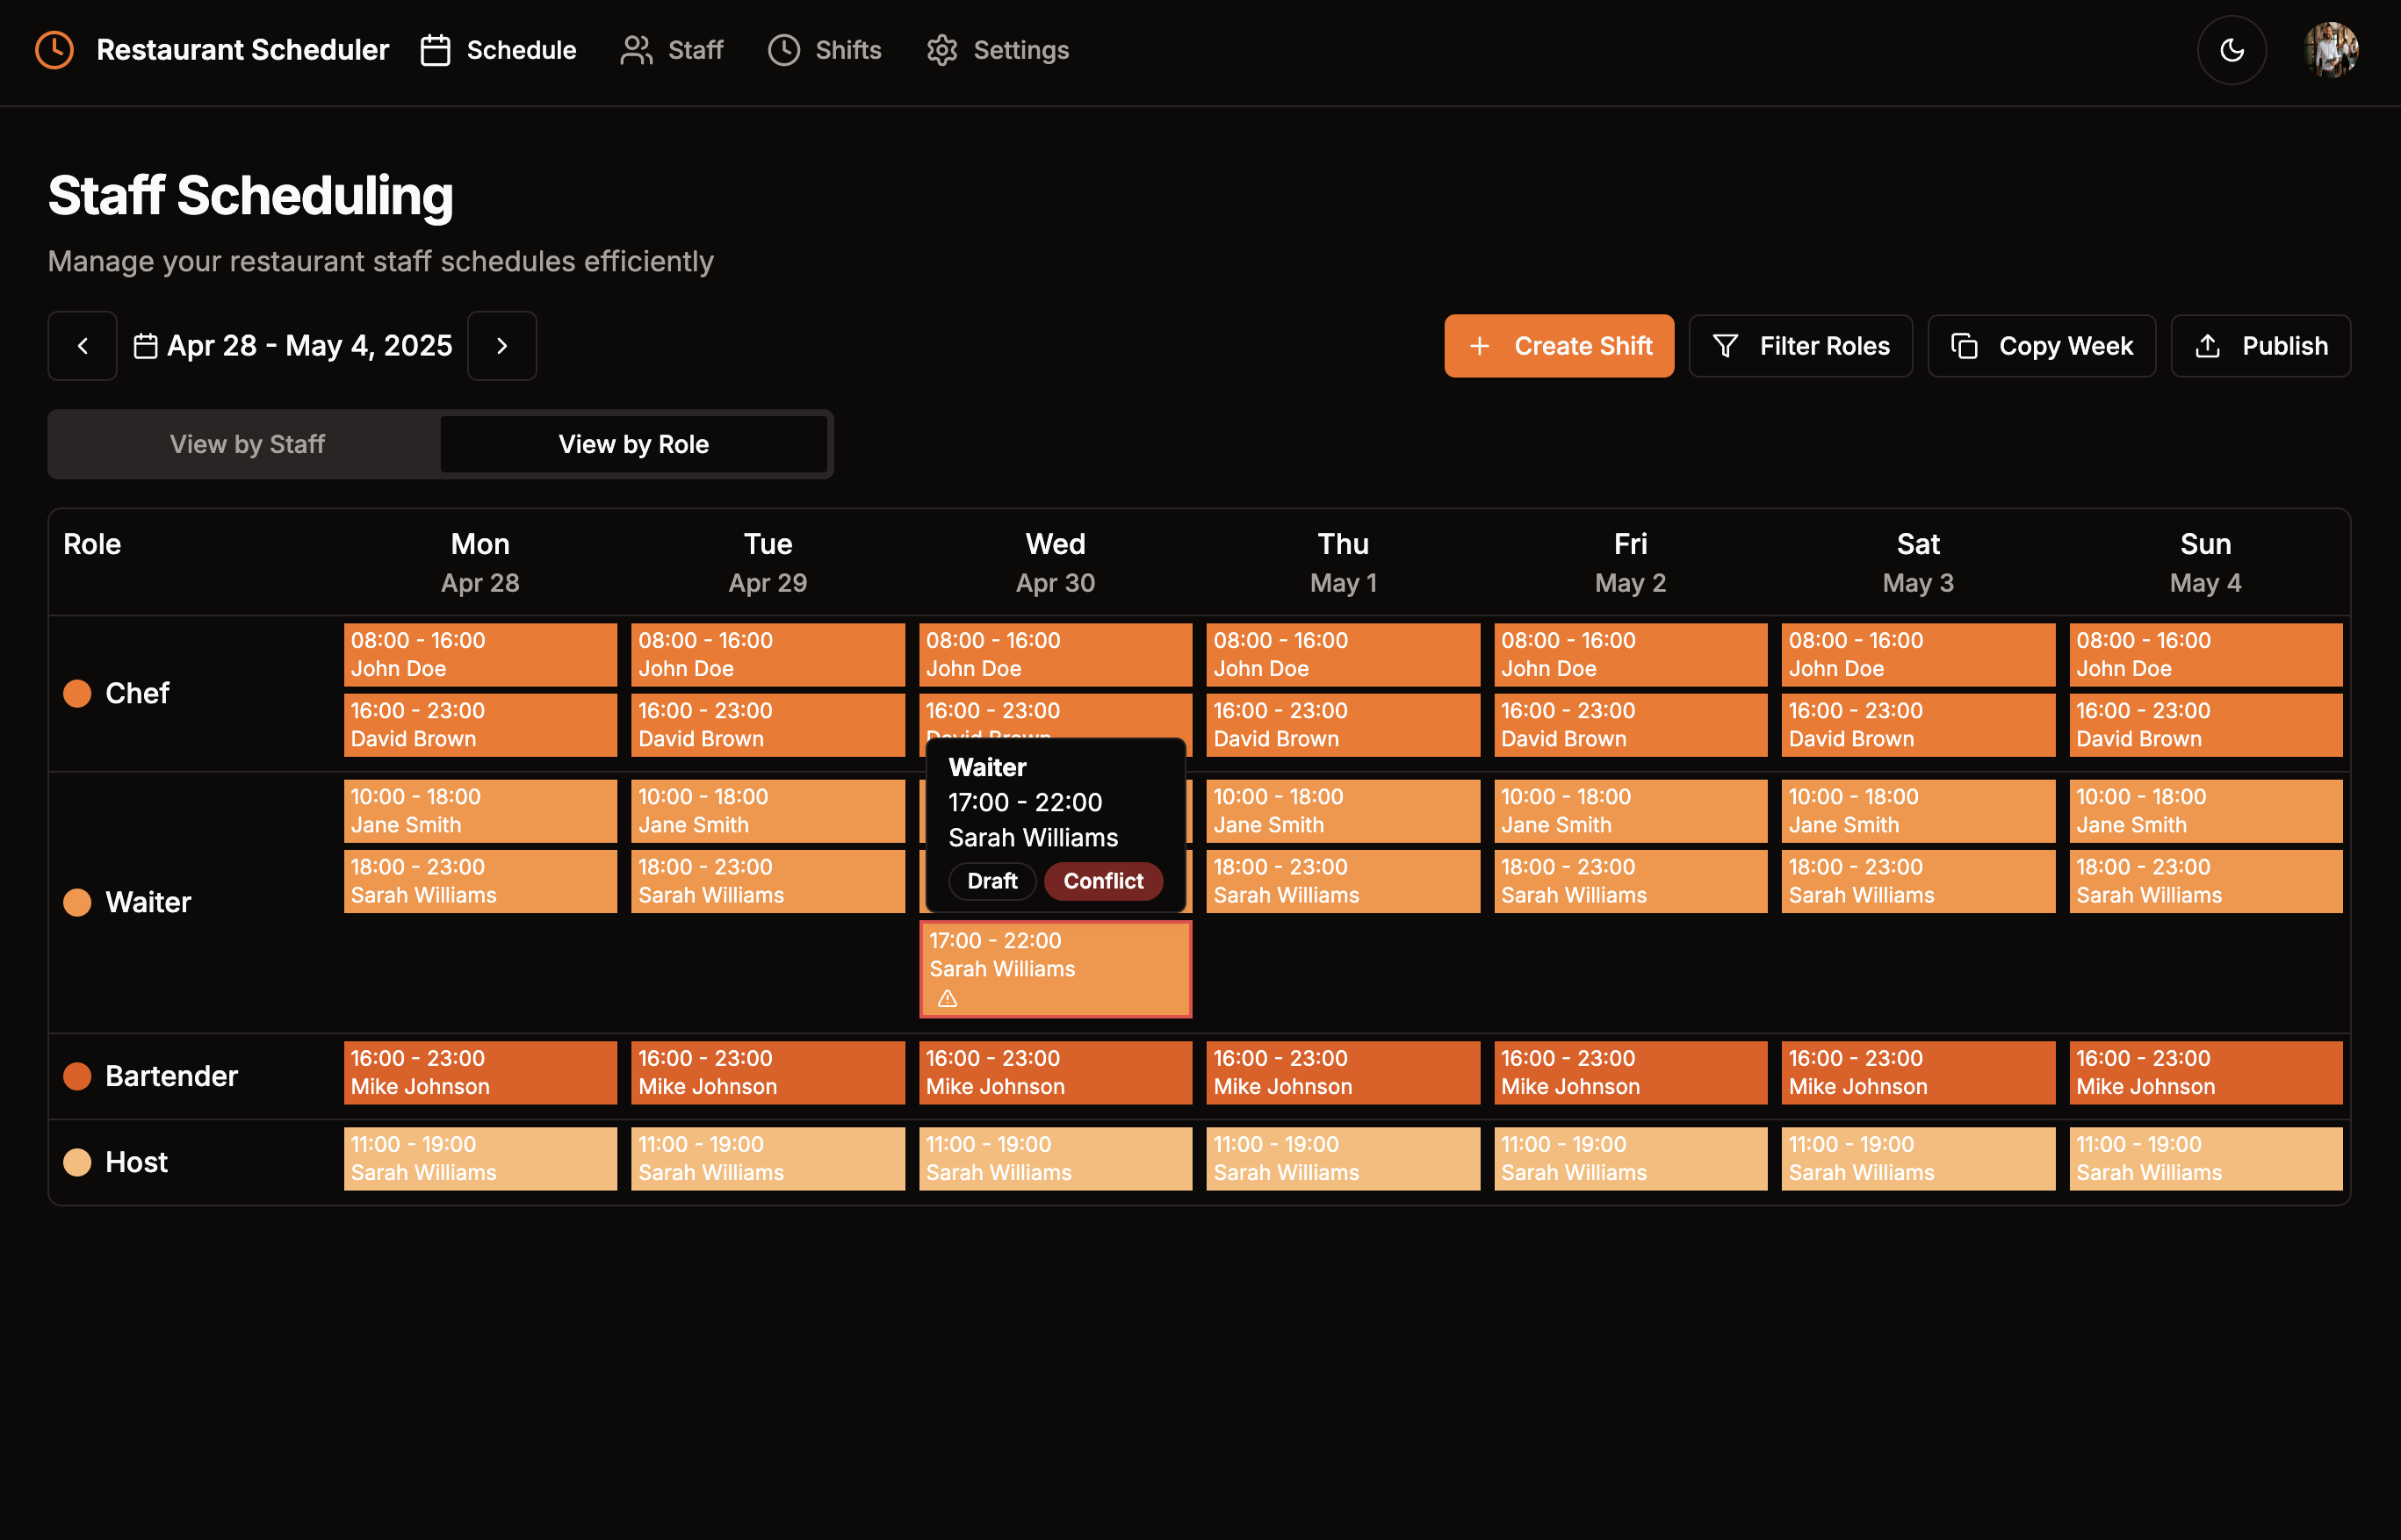
\includegraphics[width=15cm]{Sections/tong_quan/functional_spec/img/proto1.2.png}

     \vspace{0.5cm}
    \caption{Trang Dashboard (2)}
\end{figure}
\begin{figure}[H]
	\centering
	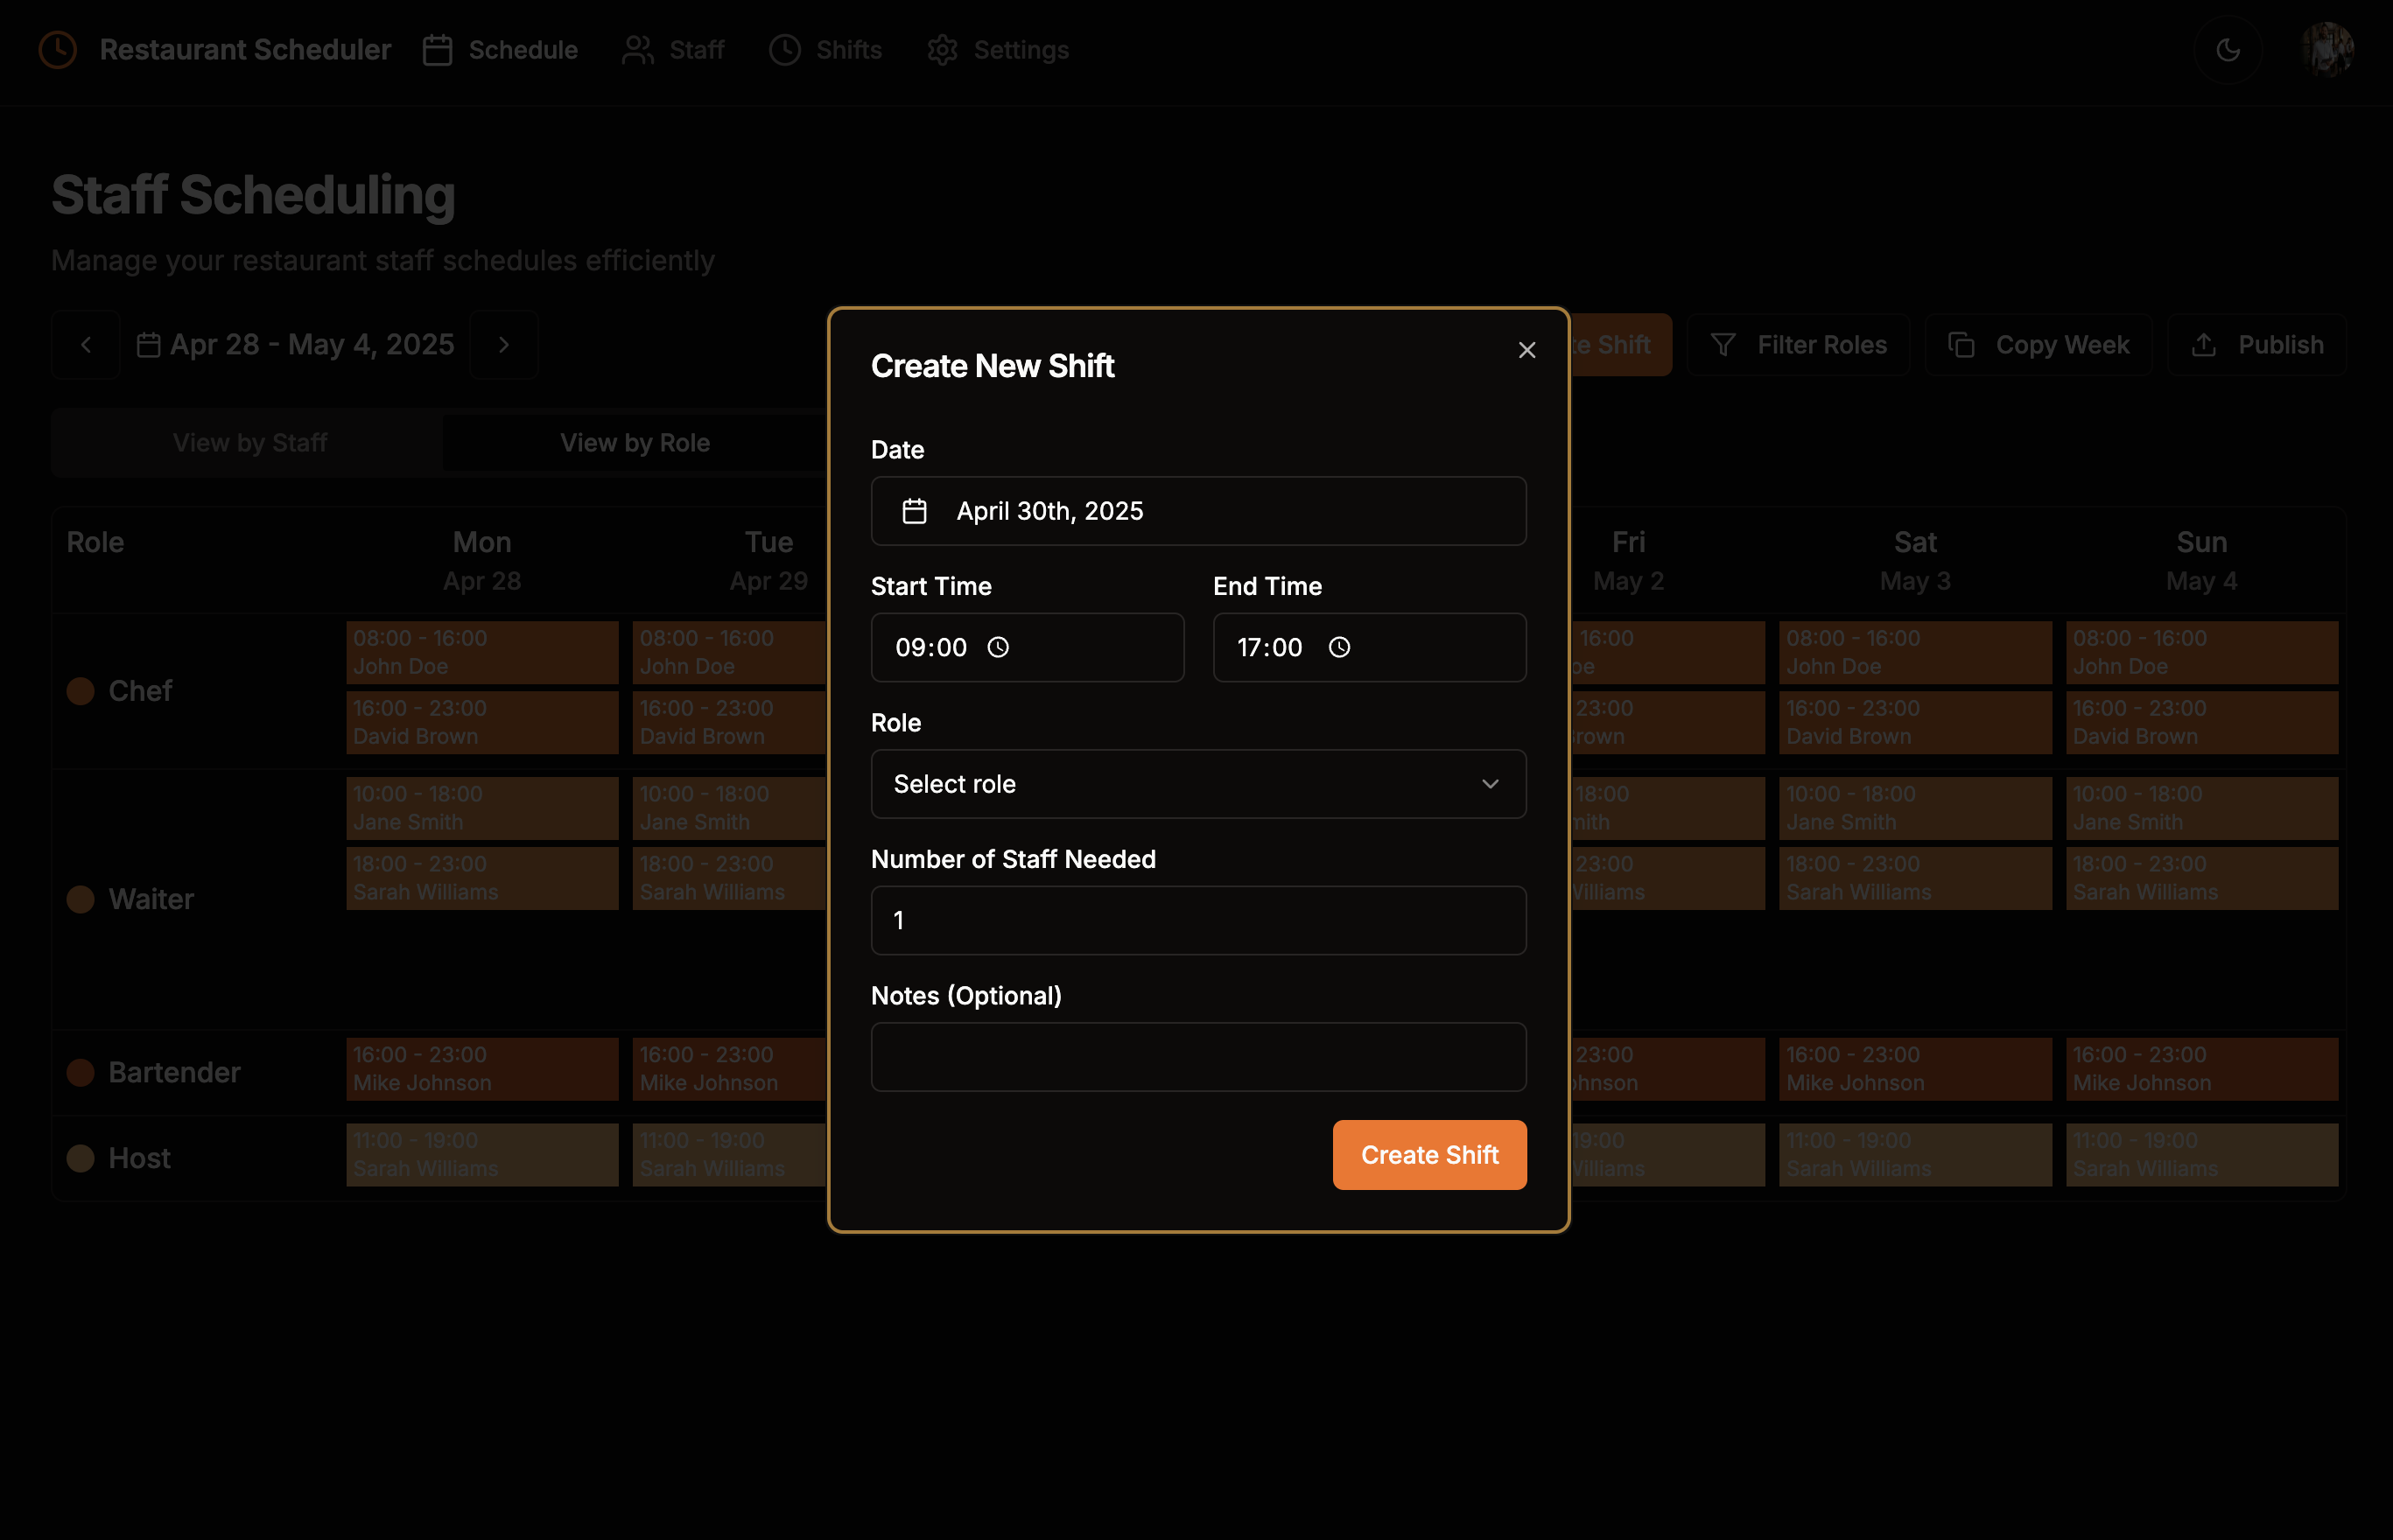
\includegraphics[width=15cm]{Sections/tong_quan/functional_spec/img/proto1.3.png}

     \vspace{0.5cm}
    \caption{Trang Dashboard (3)}
\end{figure}
\begin{figure}[H]
	\centering
	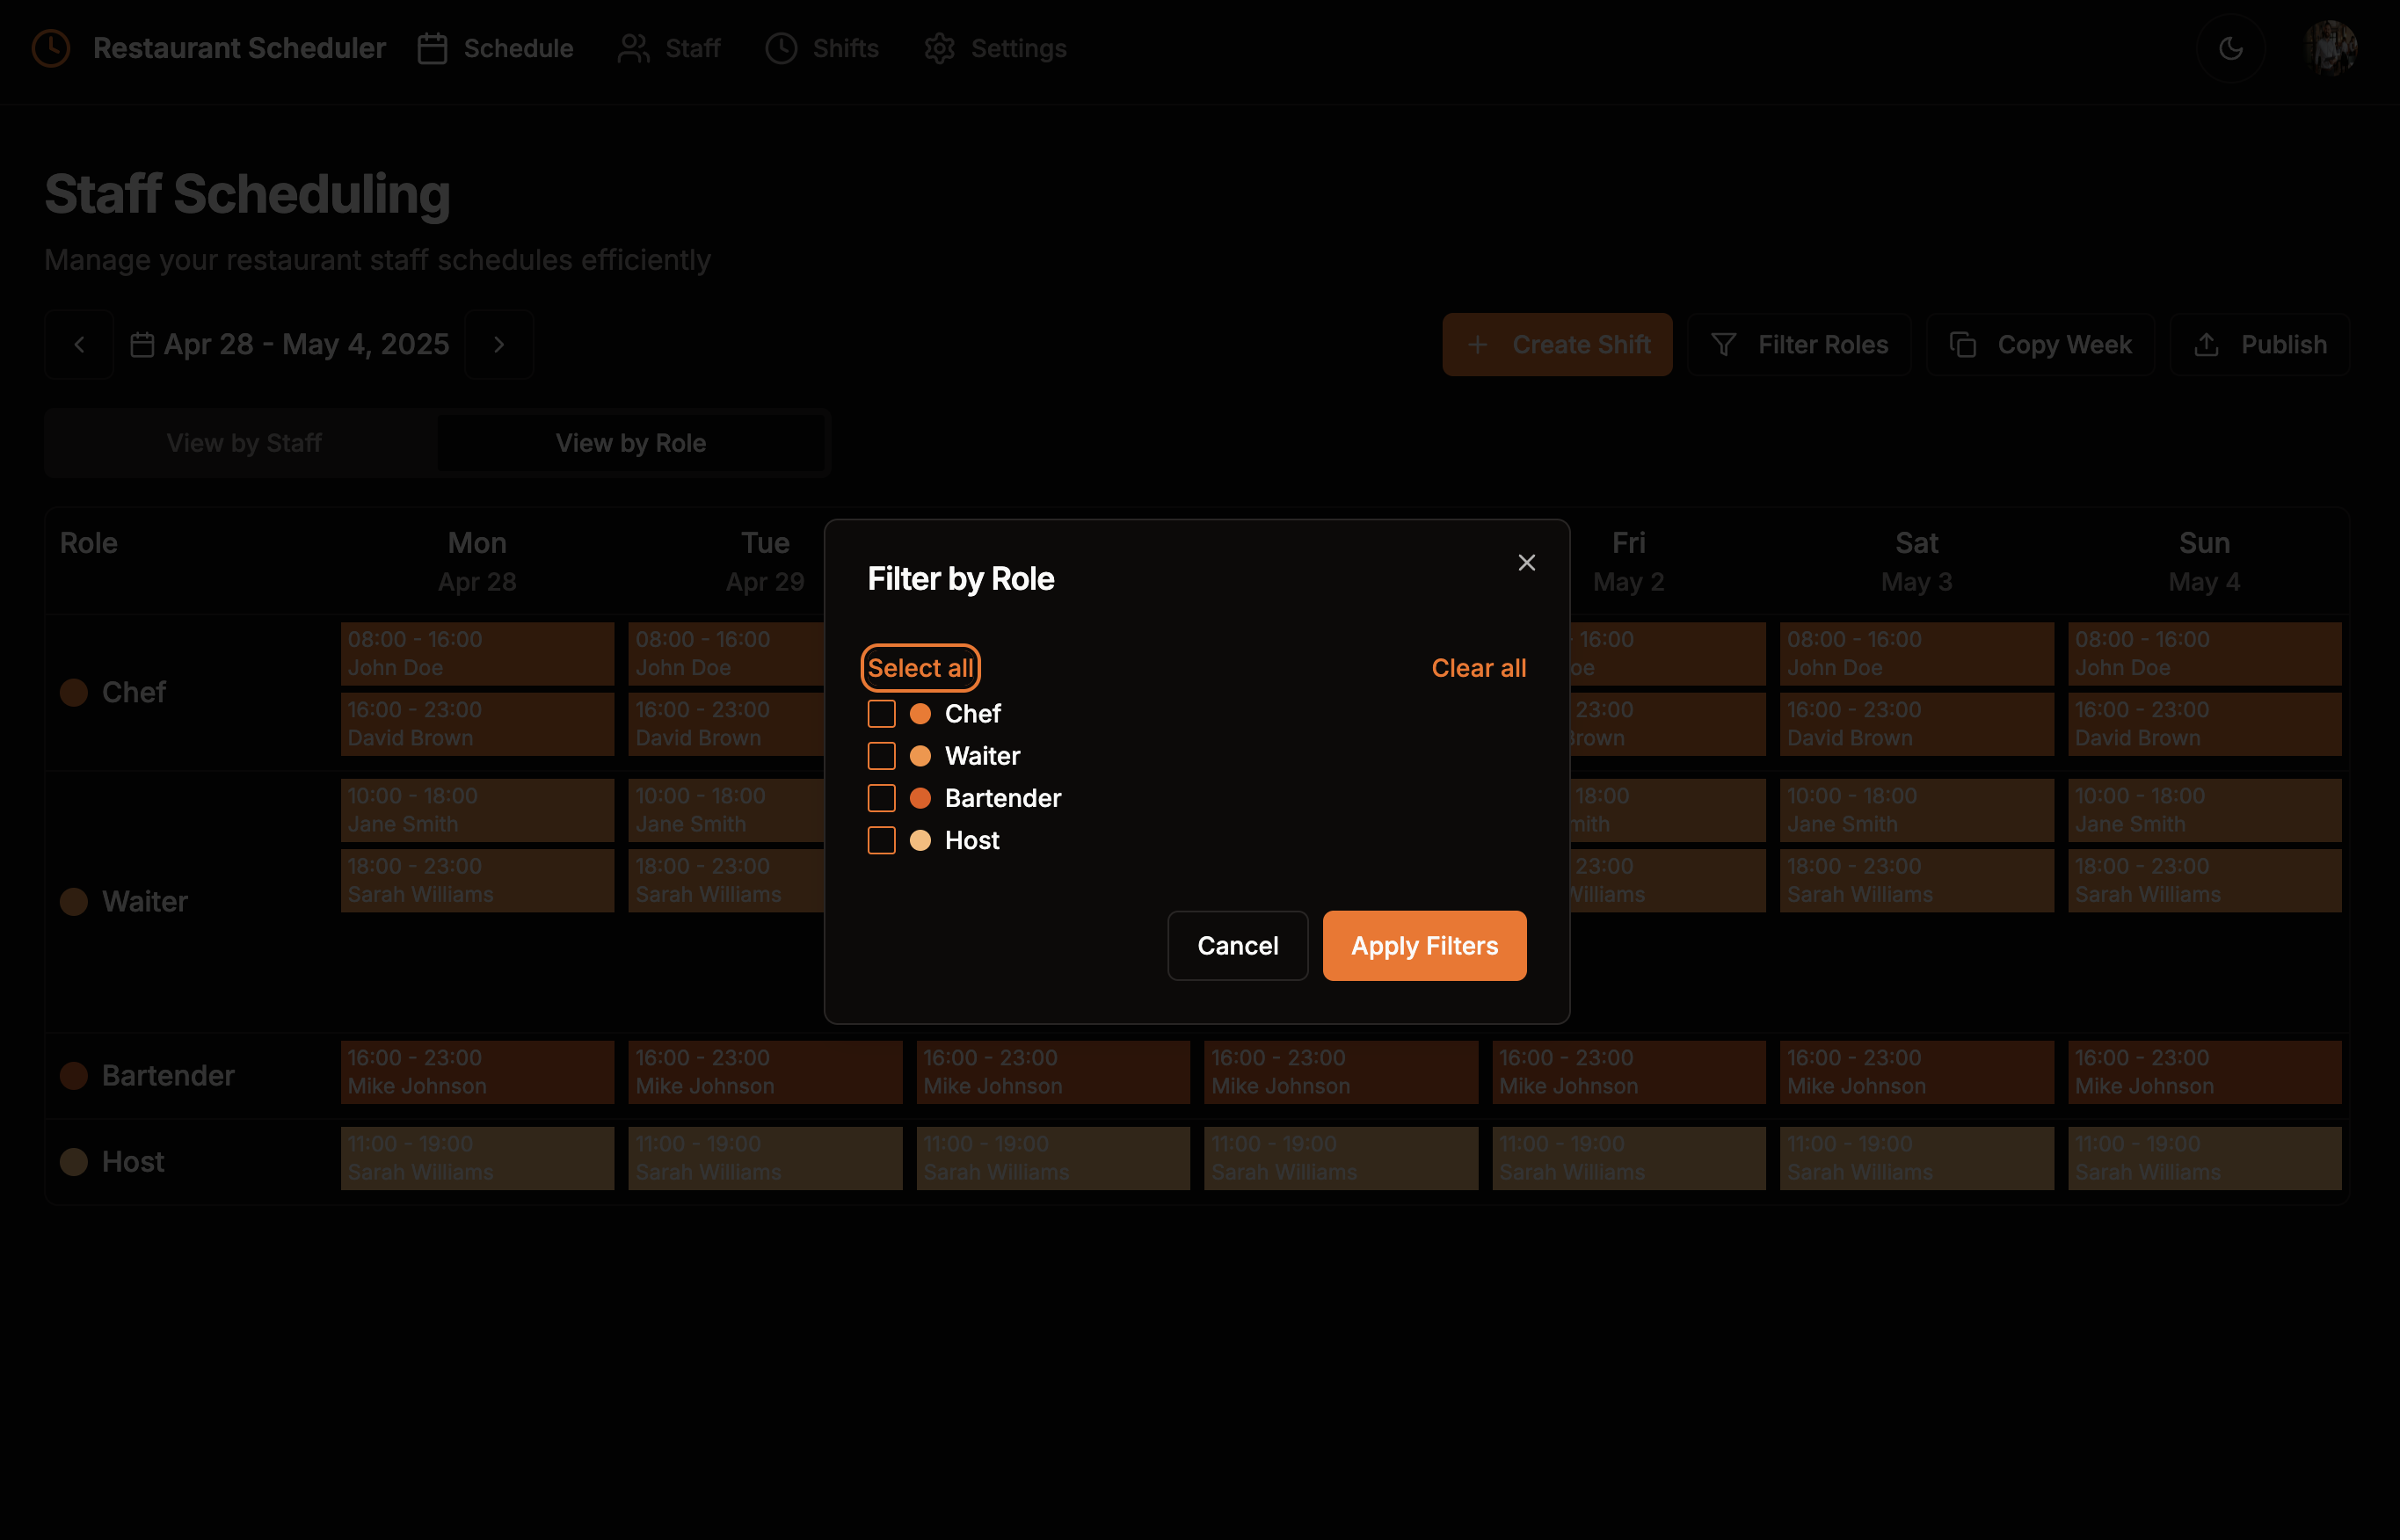
\includegraphics[width=15cm]{Sections/tong_quan/functional_spec/img/proto1.4.png}

     \vspace{0.5cm}
    \caption{Trang Dashboard (4)}
\end{figure}
\begin{figure}[H]
	\centering
	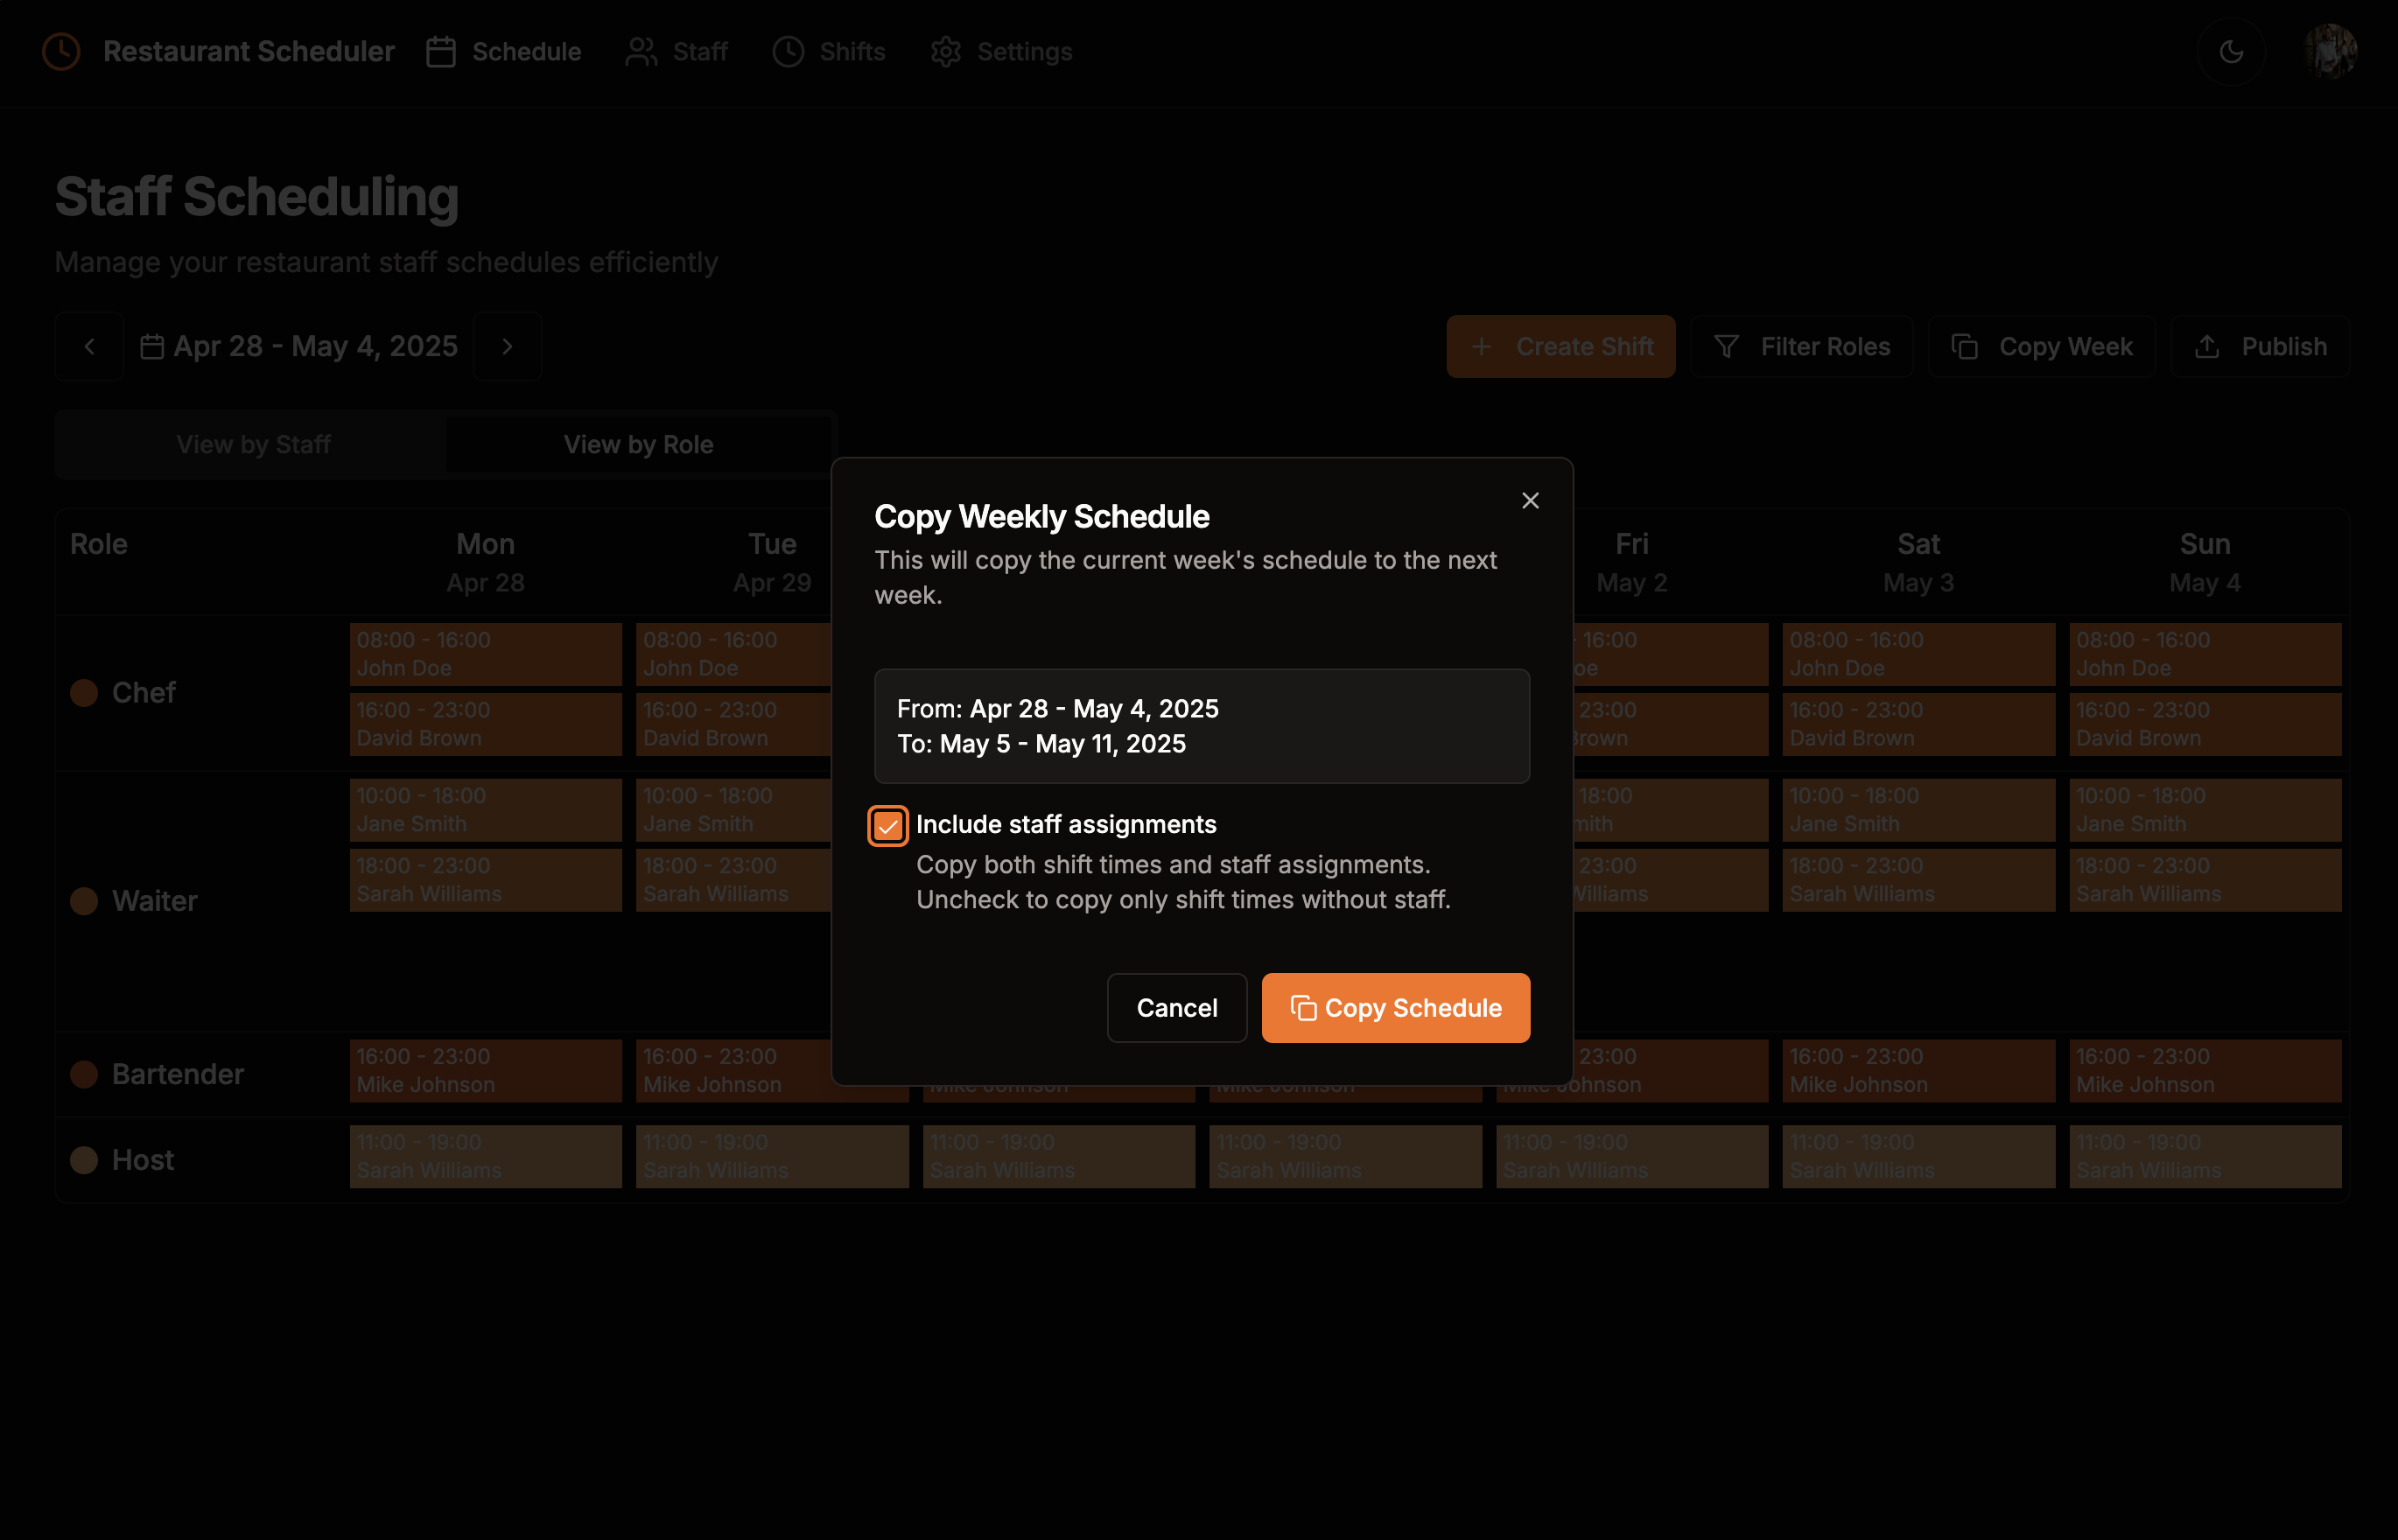
\includegraphics[width=15cm]{Sections/tong_quan/functional_spec/img/proto1.5.png}

     \vspace{0.5cm}
    \caption{Trang Dashboard (5)}
\end{figure}
\begin{figure}[H]
	\centering
	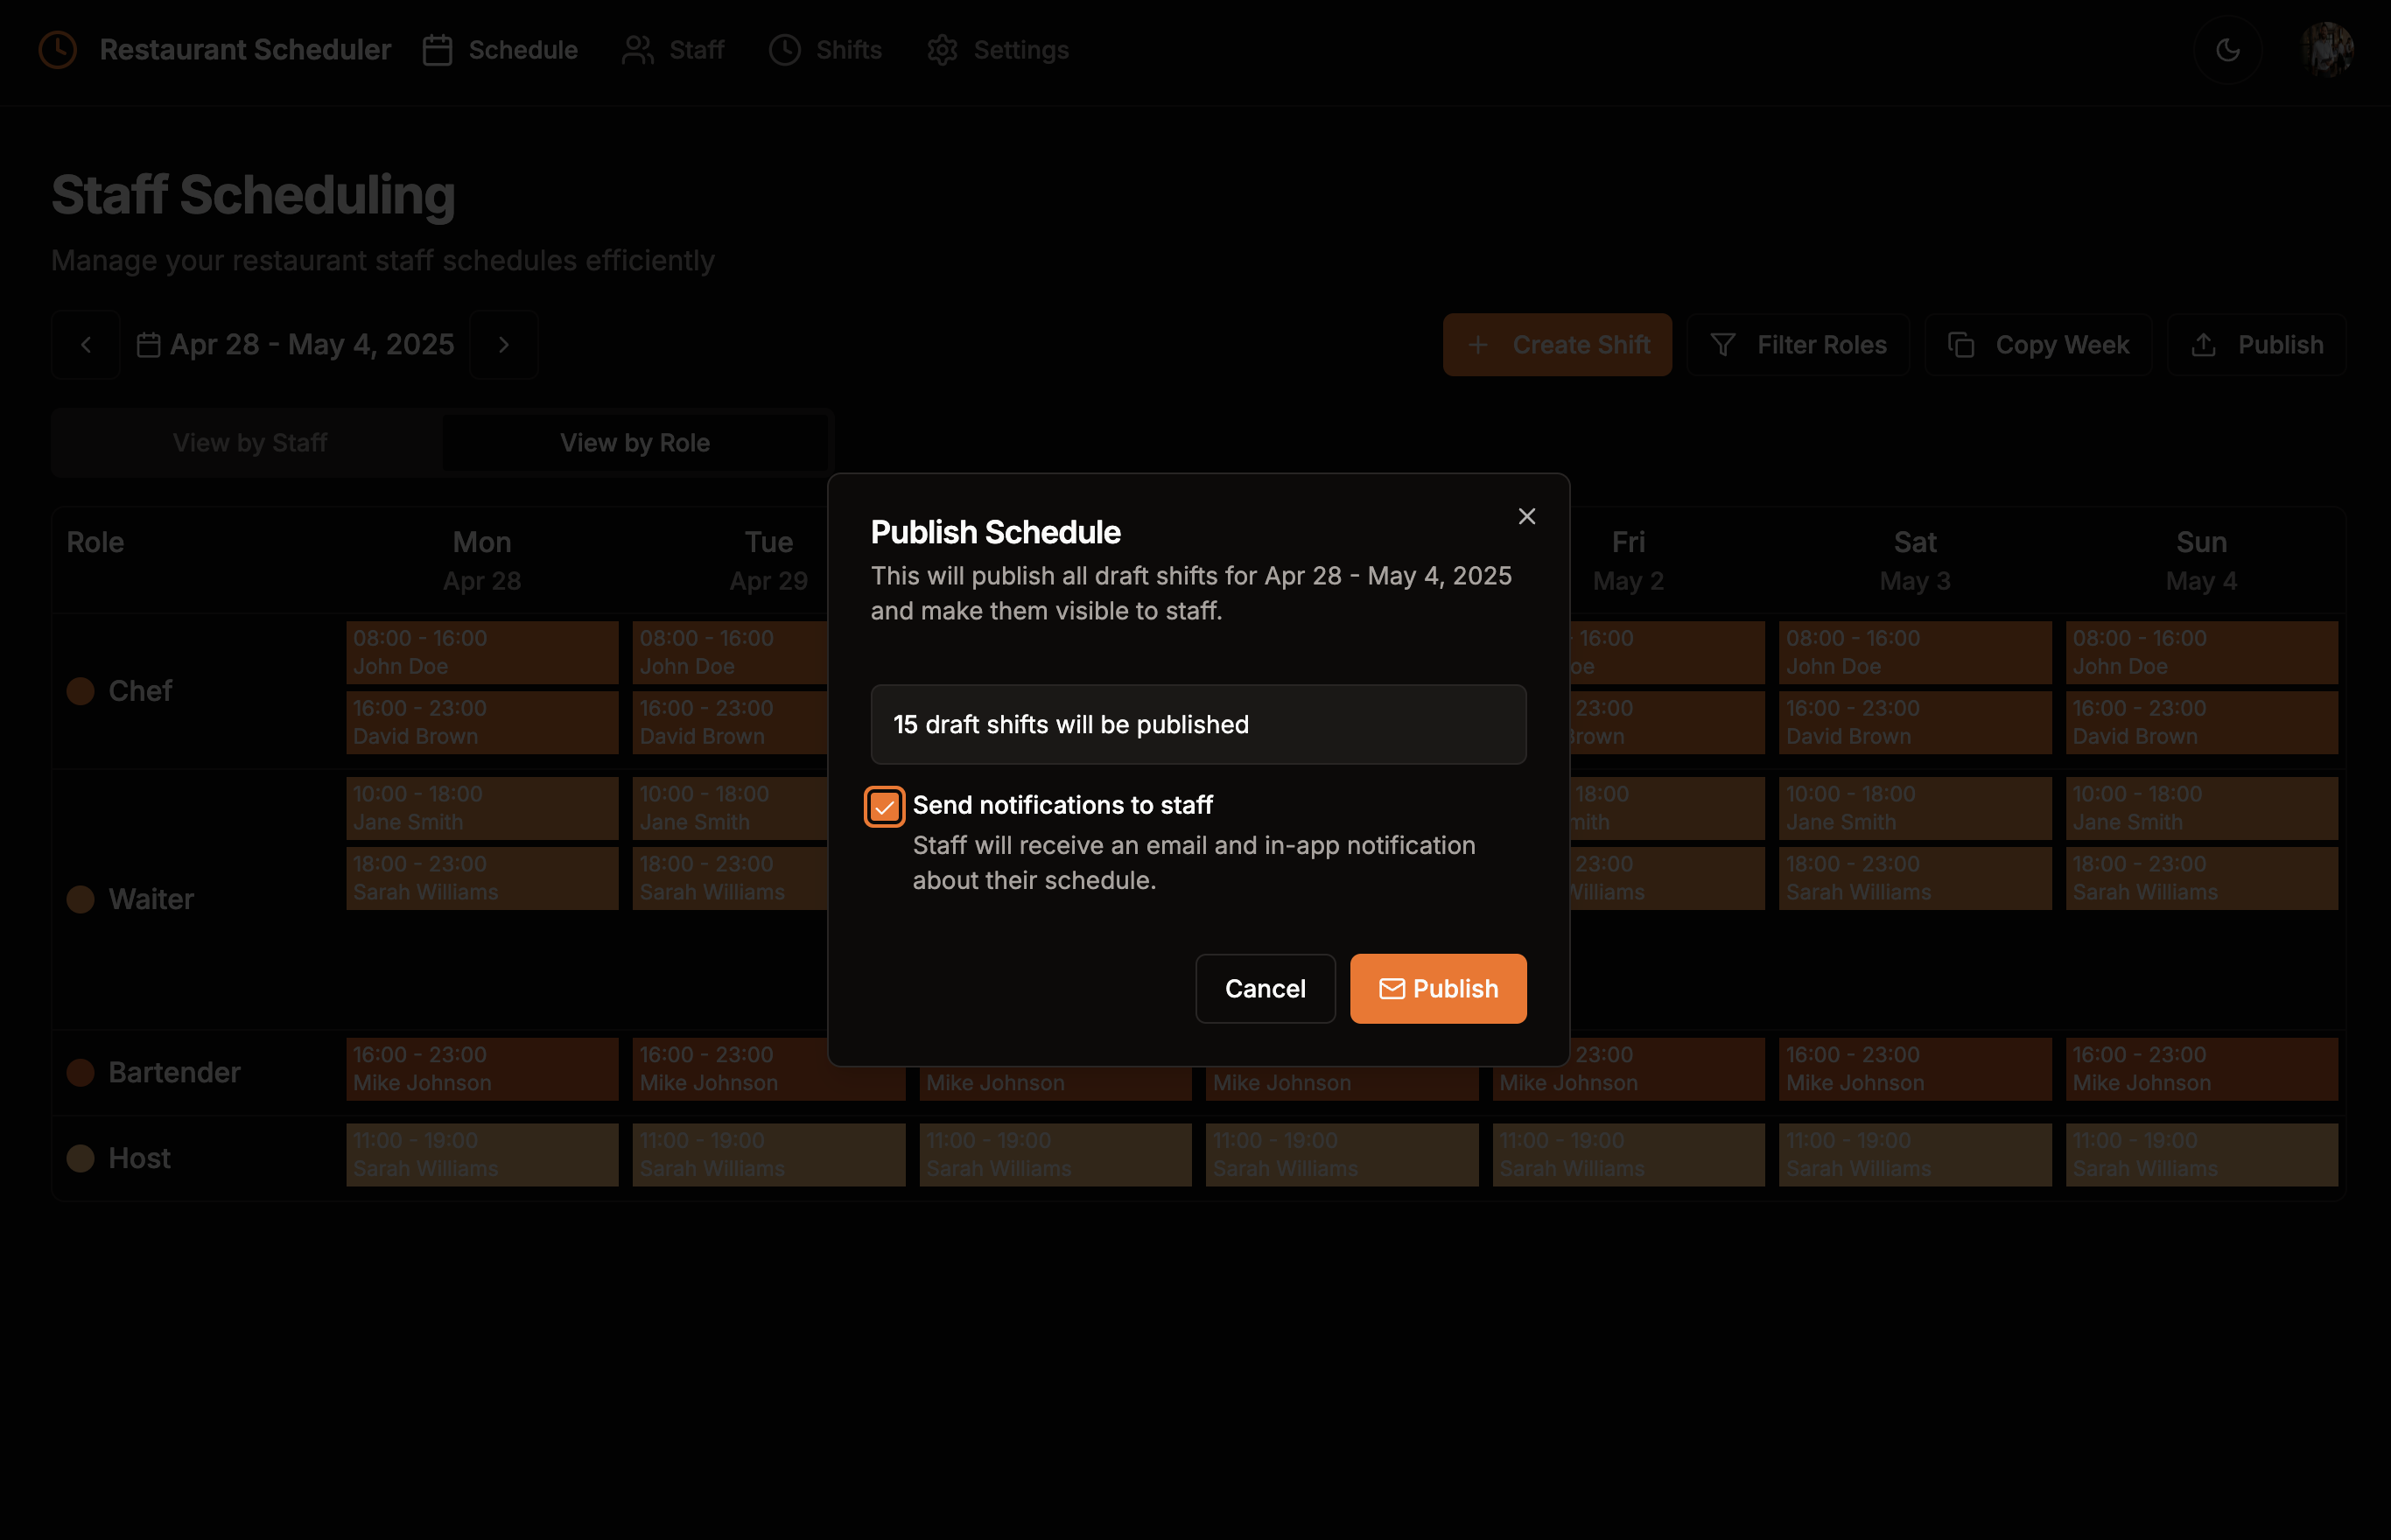
\includegraphics[width=15cm]{Sections/tong_quan/functional_spec/img/proto1.6.png}

     \vspace{0.5cm}
    \caption{Trang Staff Management}
\end{figure}
\begin{figure}[H]
	\centering
	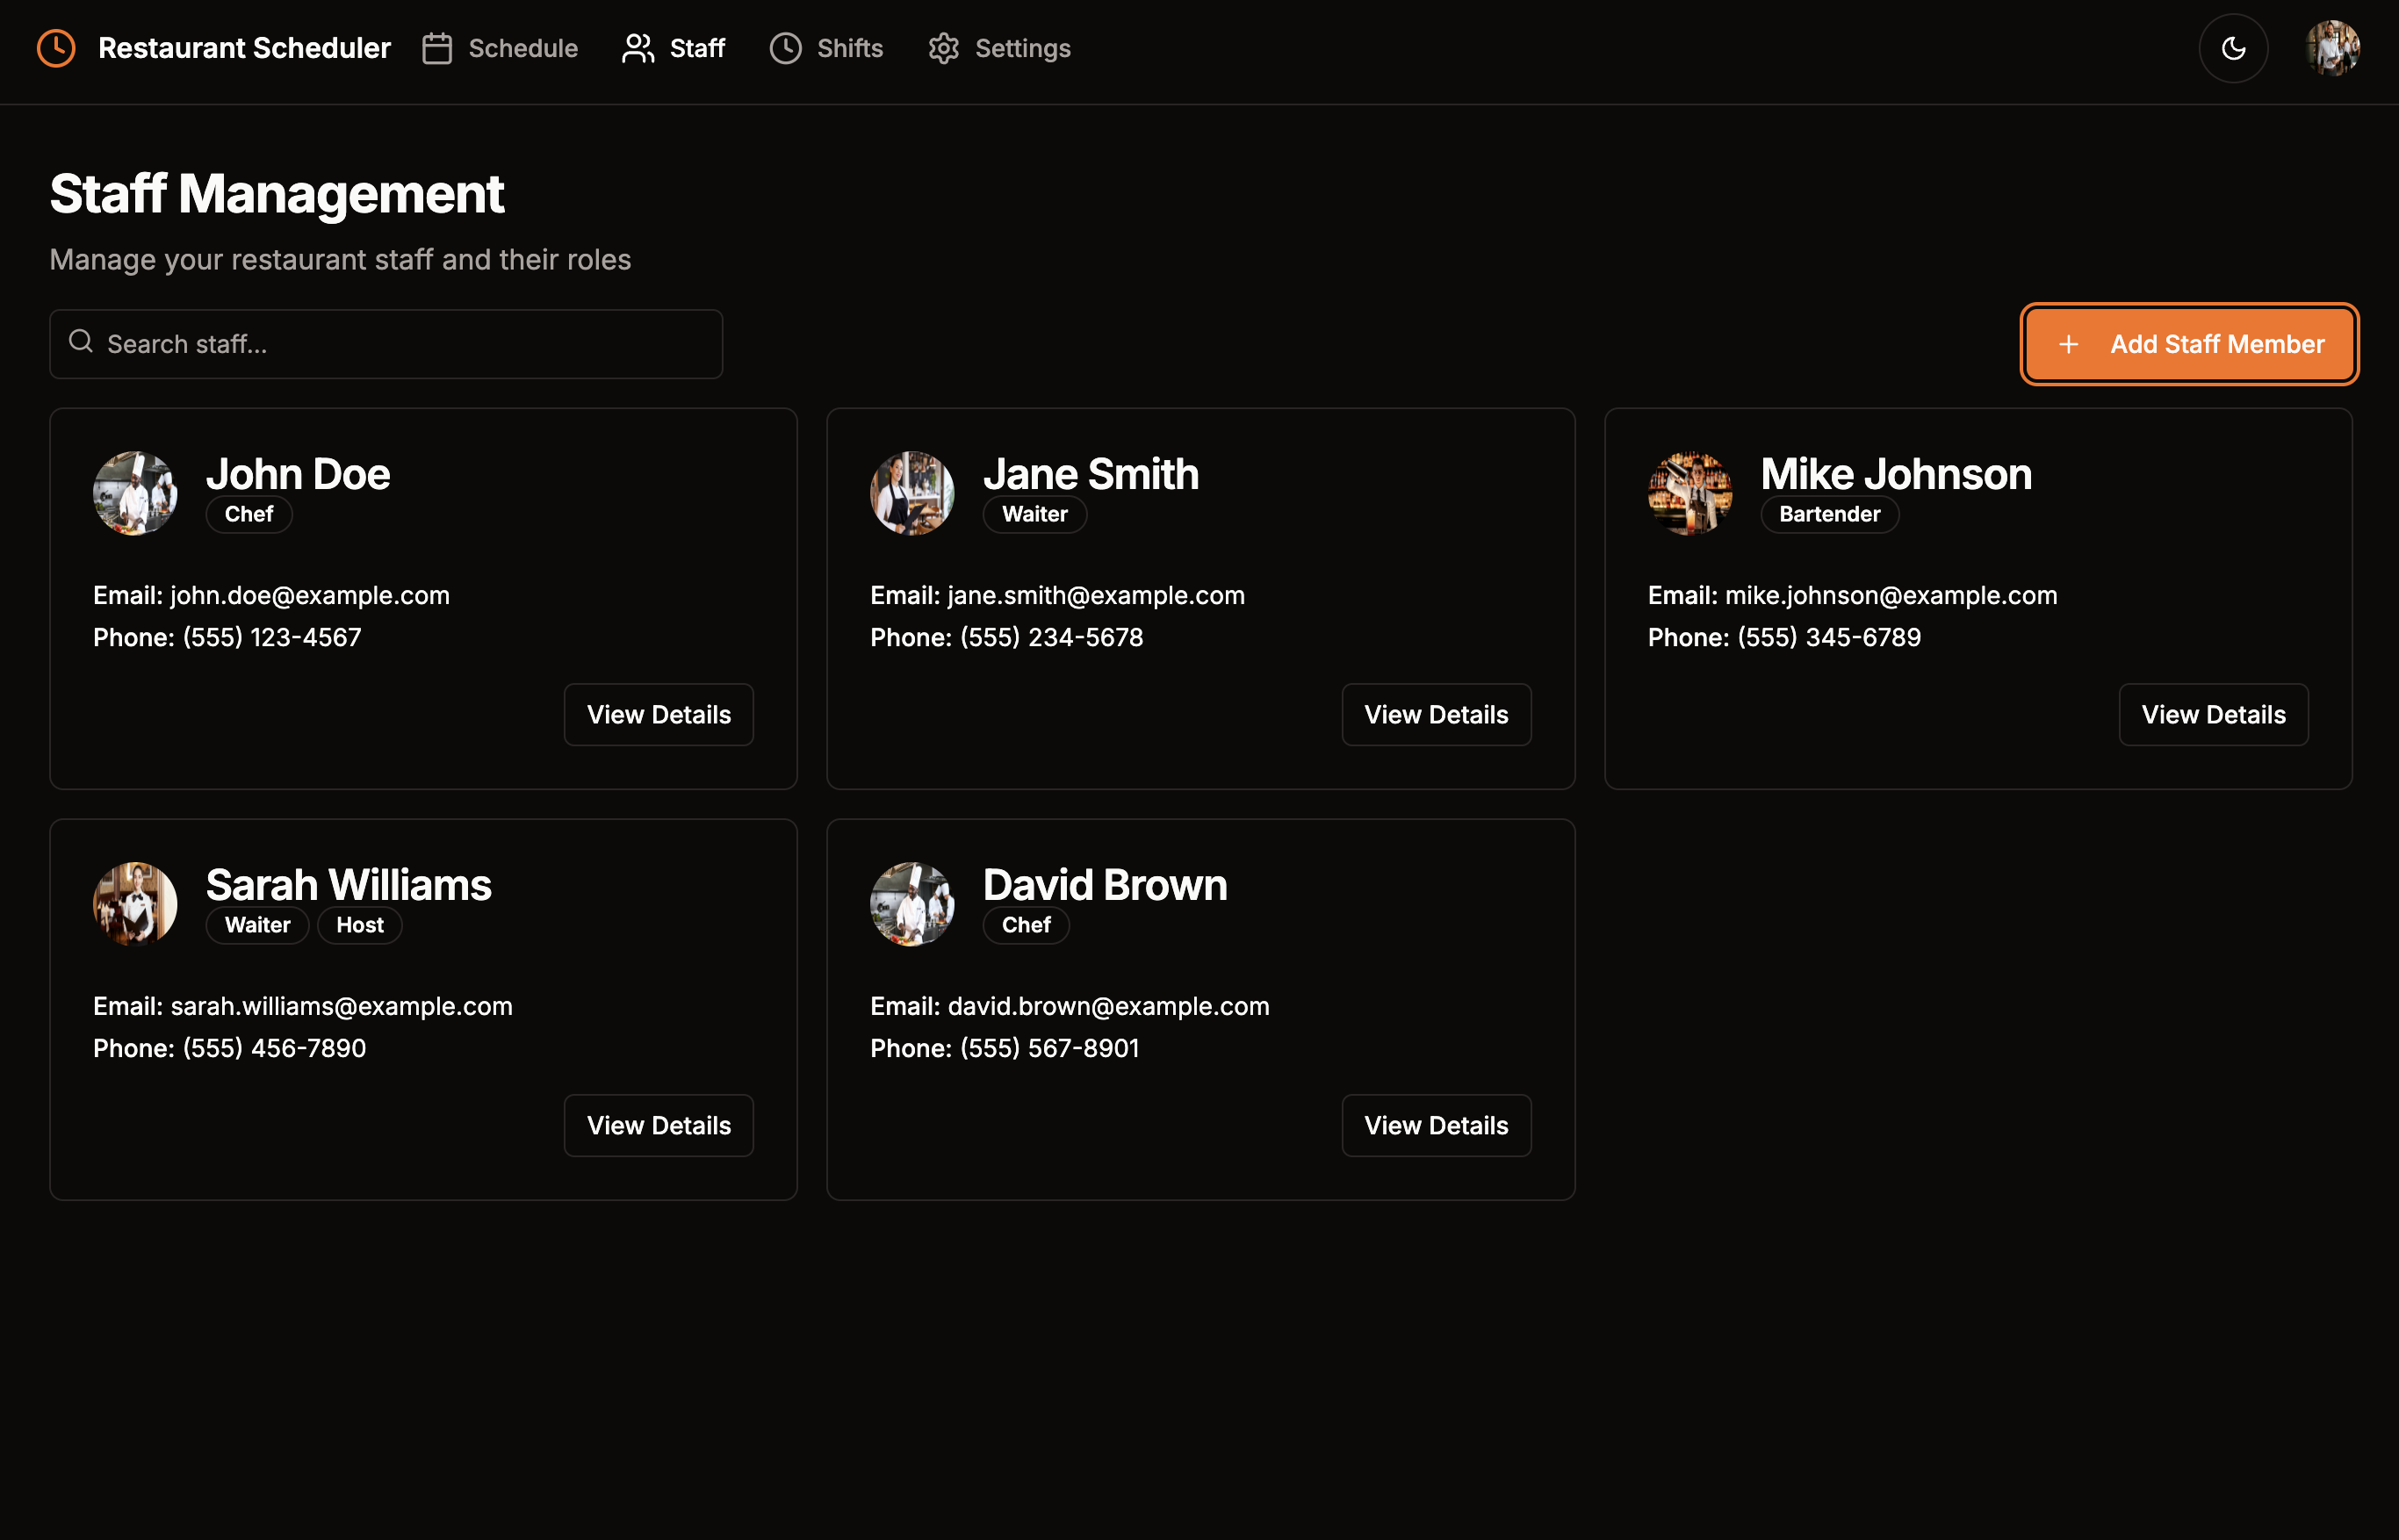
\includegraphics[width=15cm]{Sections/tong_quan/functional_spec/img/proto1.7.png}

     \vspace{0.5cm}
    \caption{Trang Shift Management}
\end{figure}
\begin{figure}[H]
	\centering
	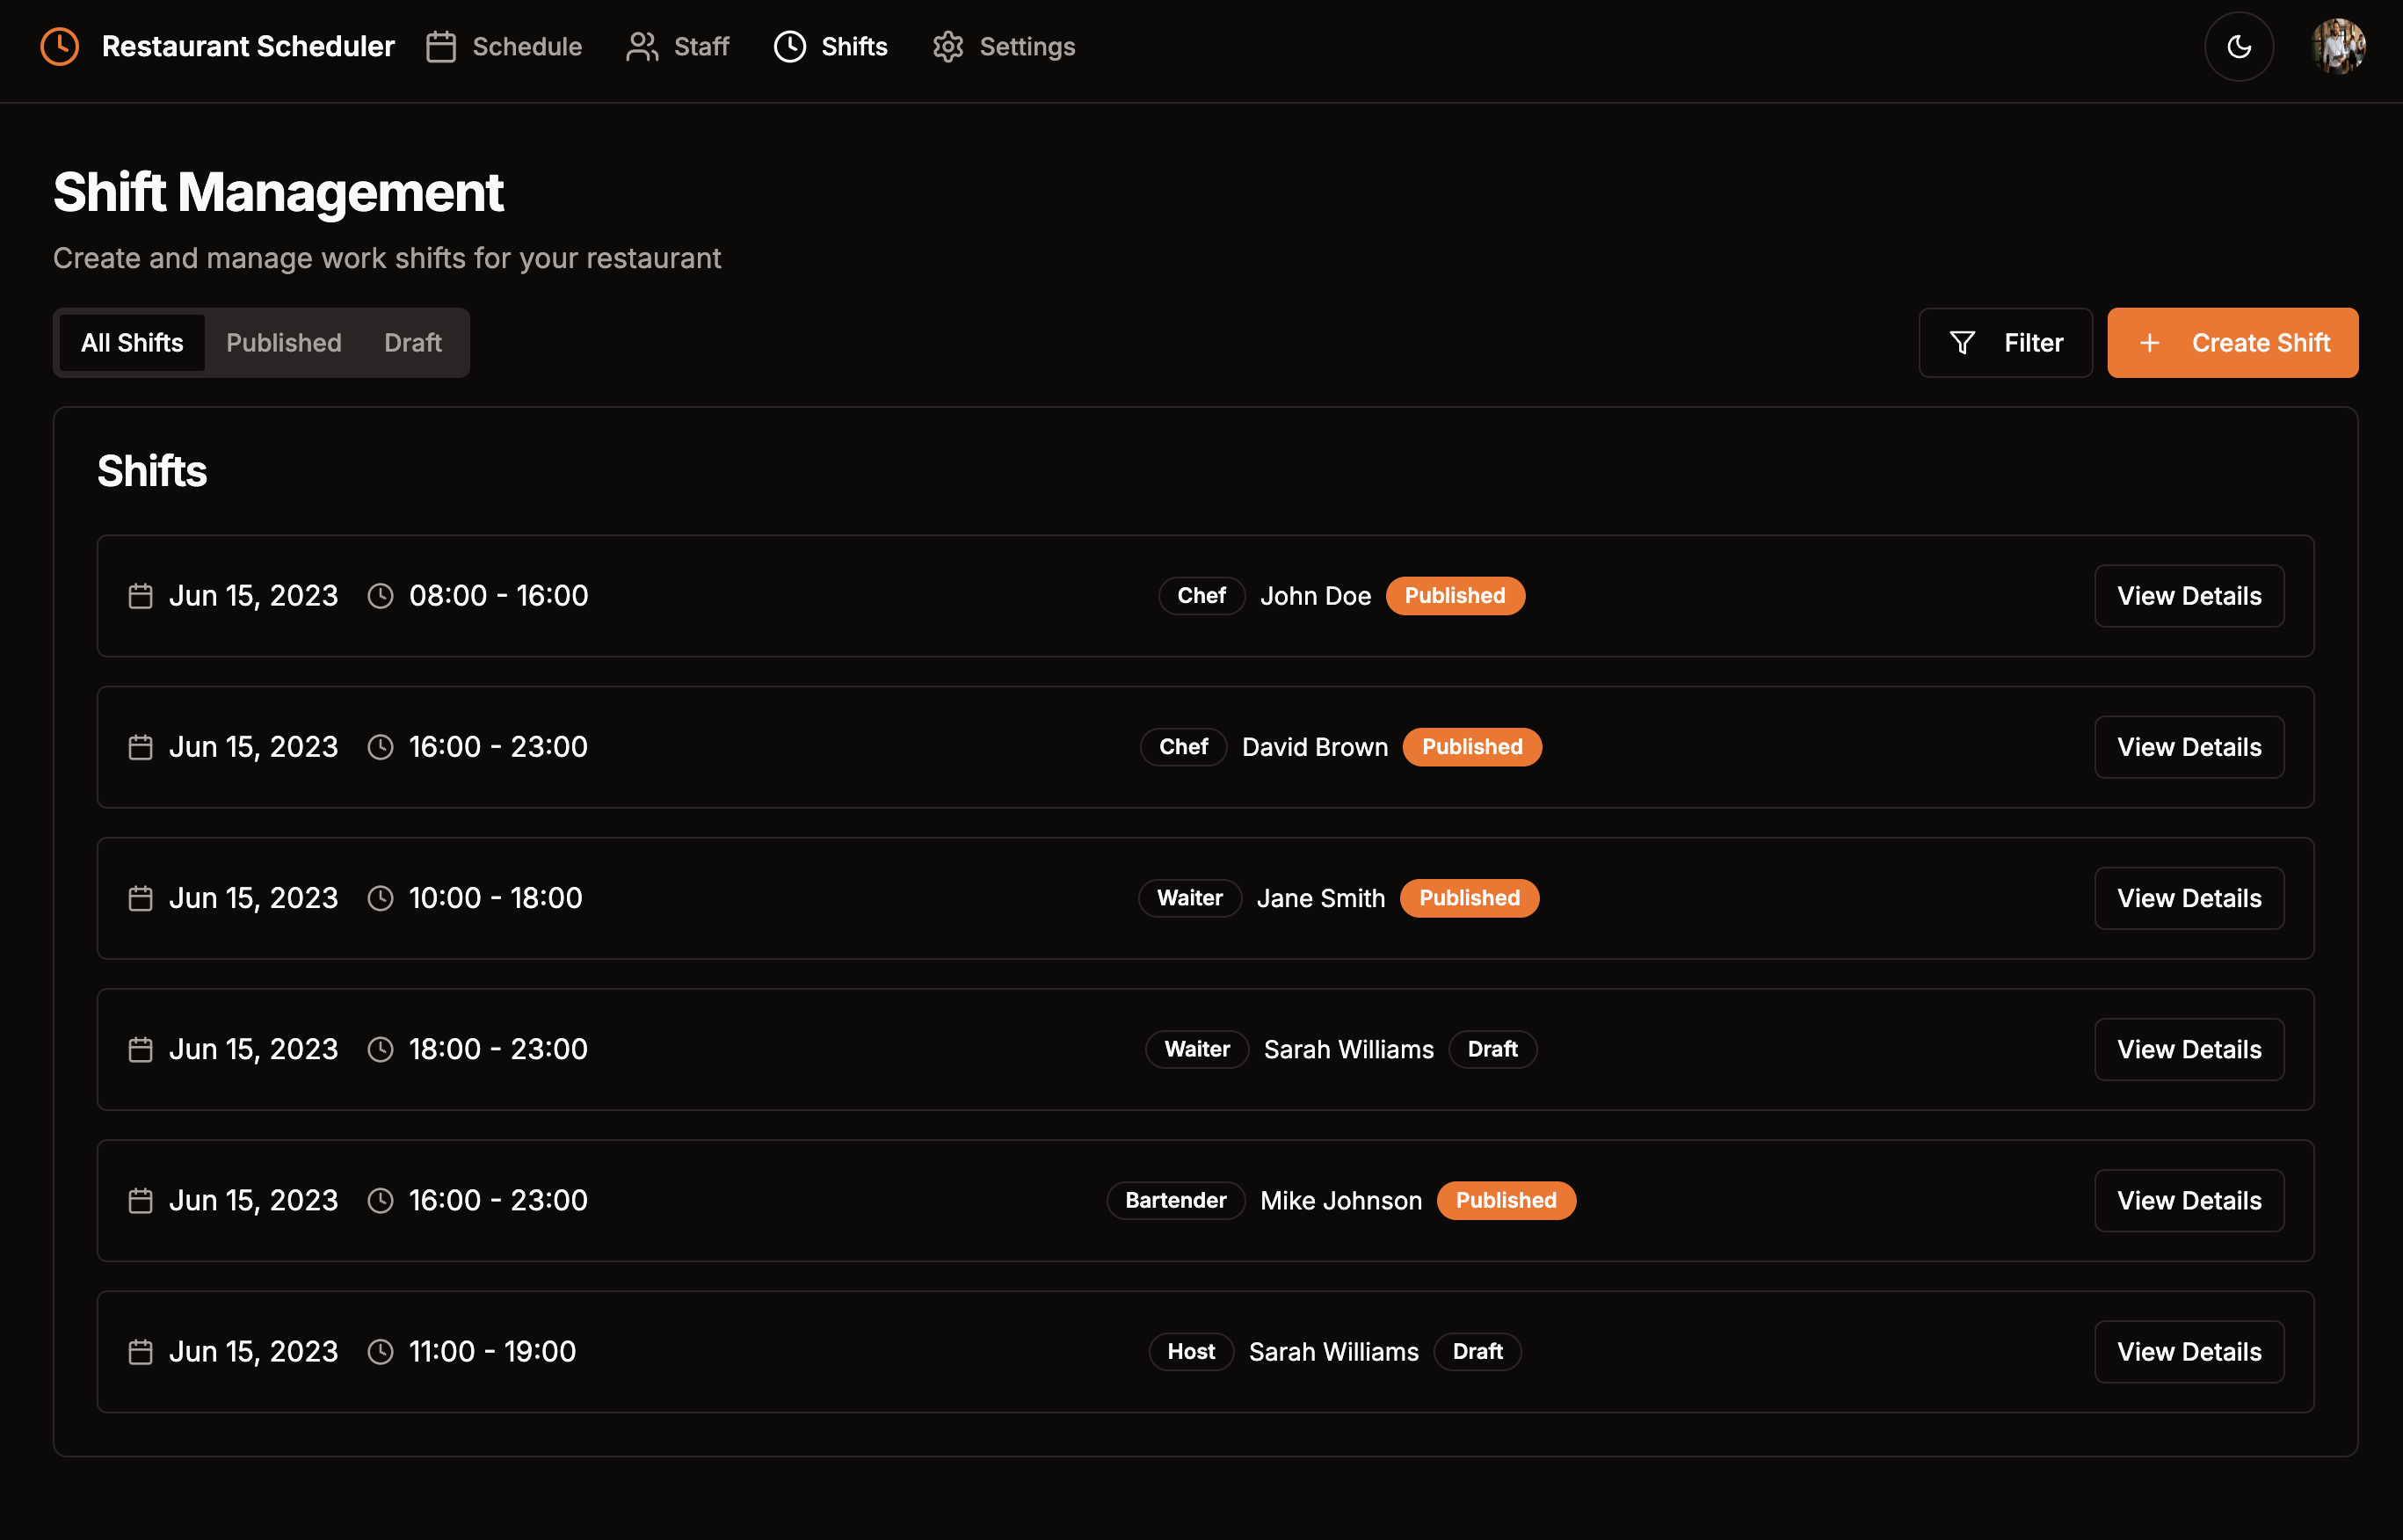
\includegraphics[width=15cm]{Sections/tong_quan/functional_spec/img/proto1.8.png}

     \vspace{0.5cm}
    \caption{Trang Settings (1)}
\end{figure}
\begin{figure}[H]
	\centering
	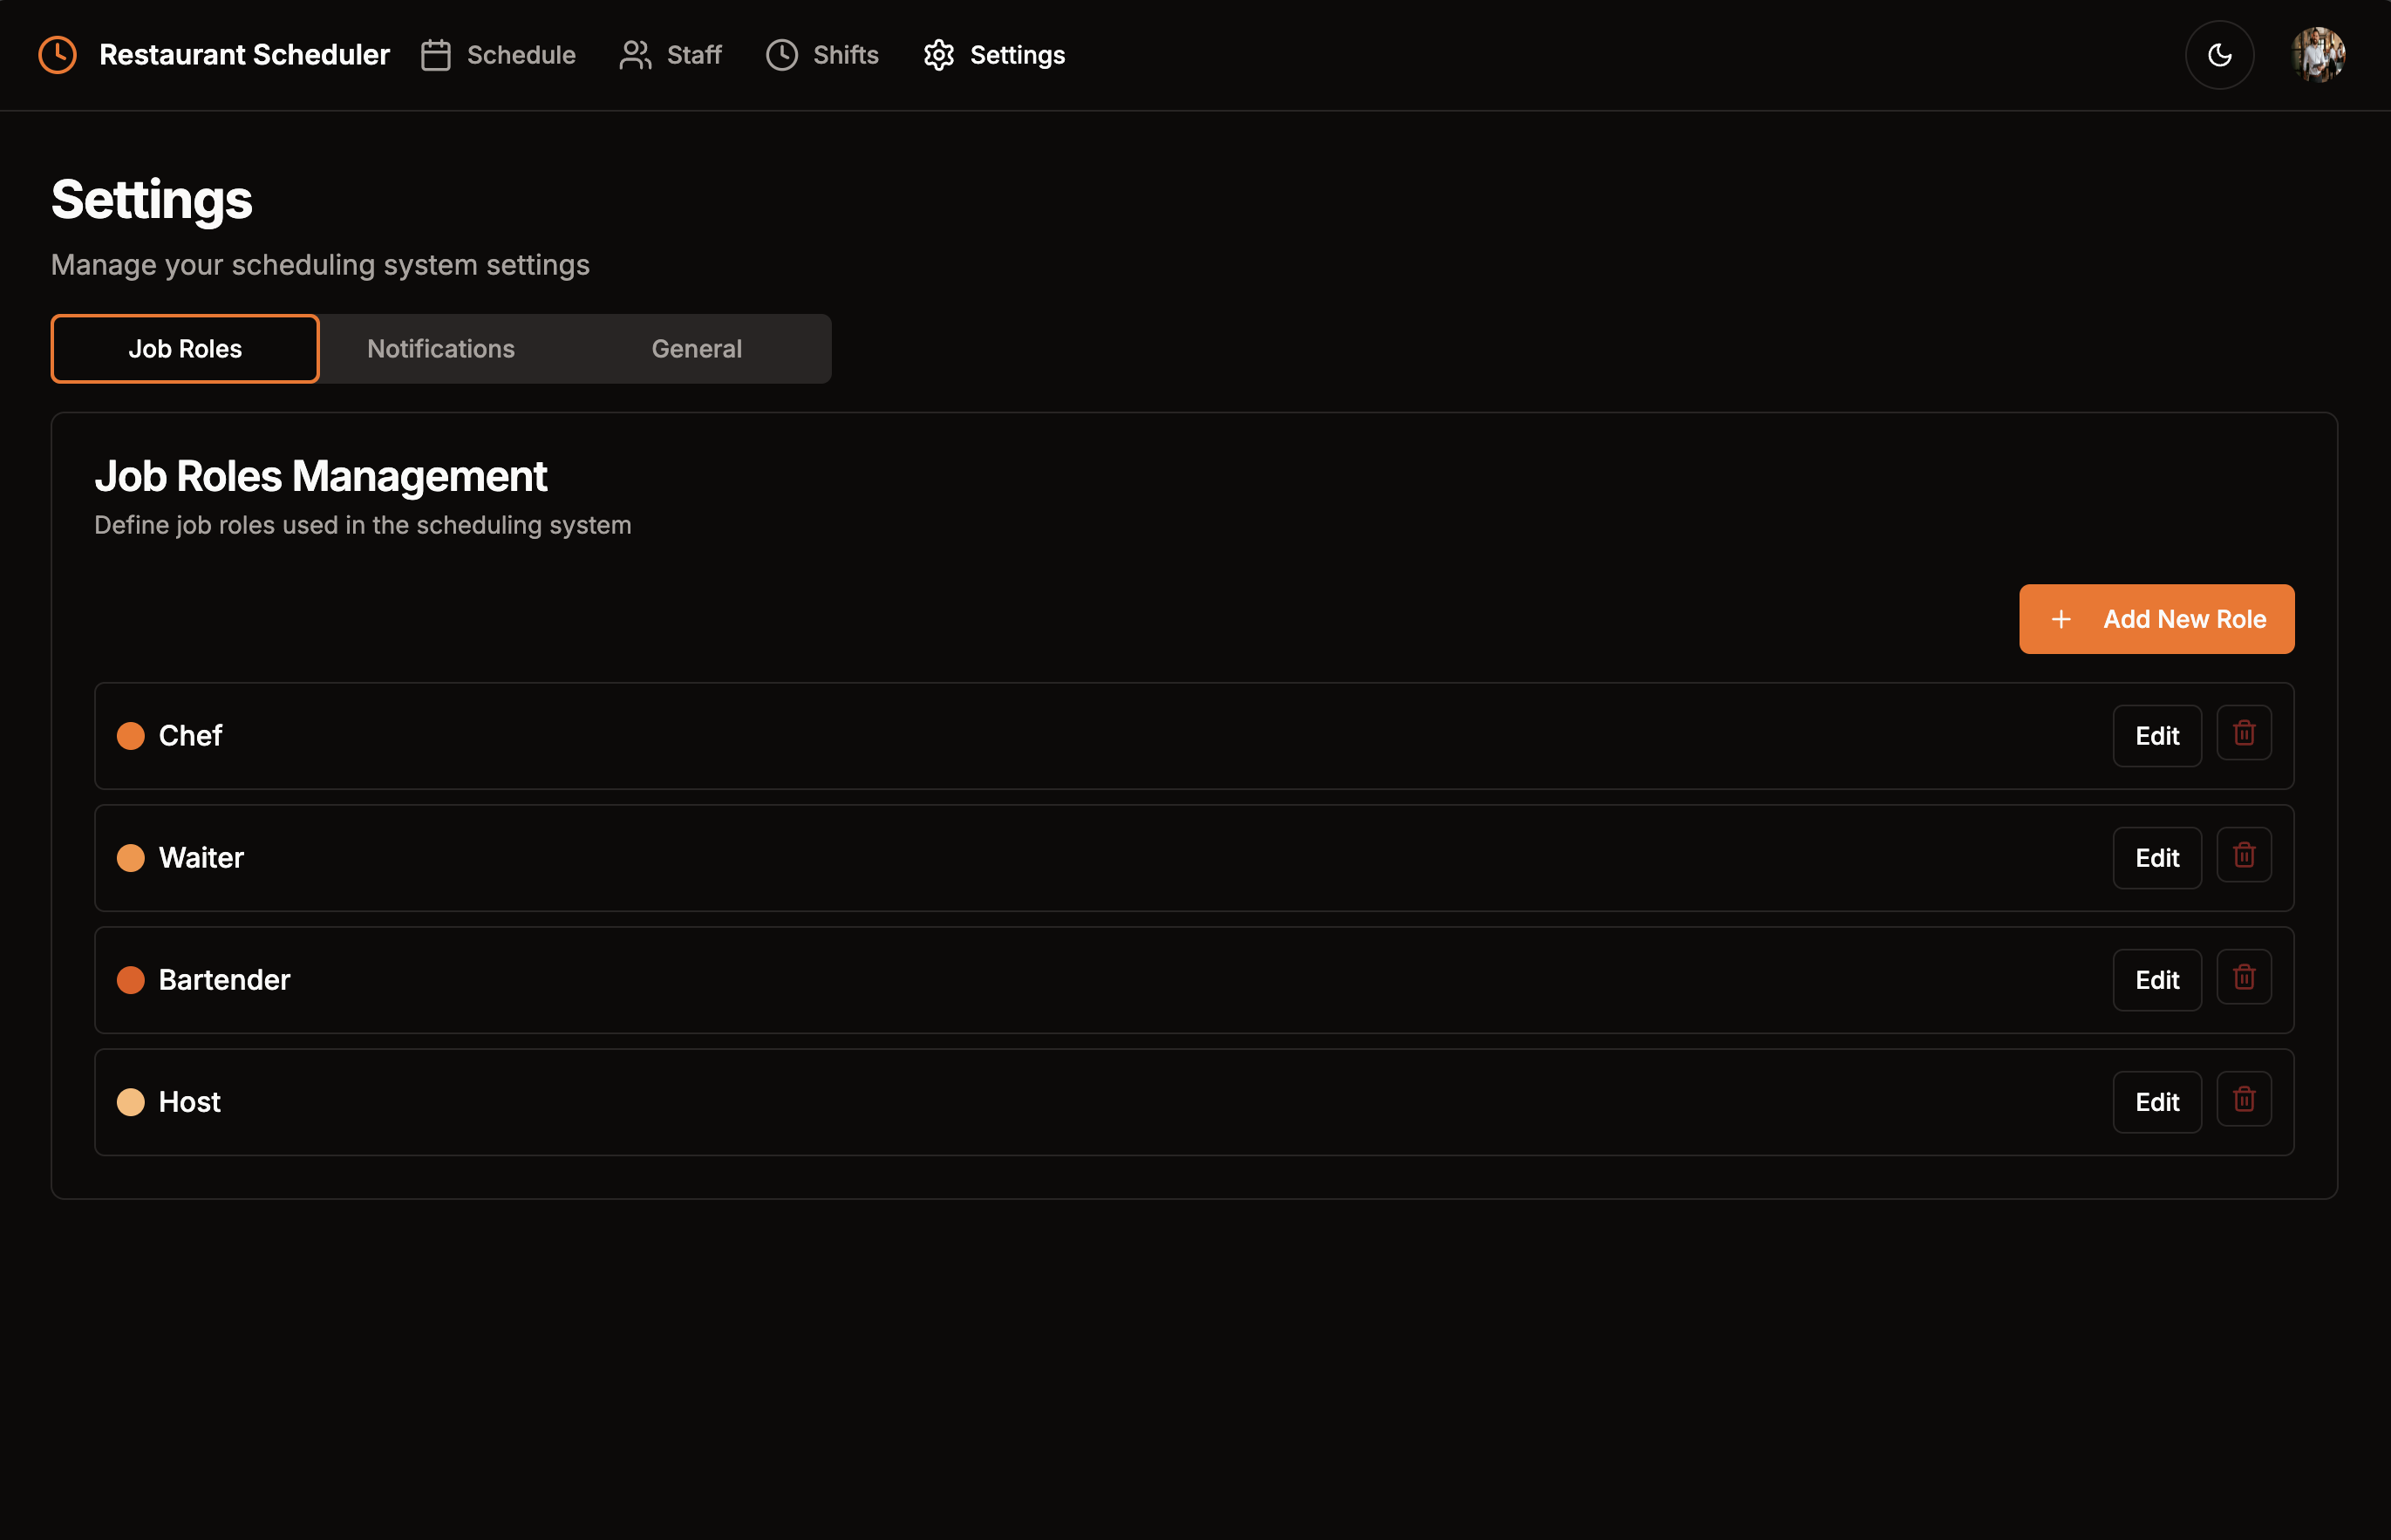
\includegraphics[width=15cm]{Sections/tong_quan/functional_spec/img/proto1.9.png}

     \vspace{0.5cm}
    \caption{Trang Settings (2)}
\end{figure}
\begin{figure}[H]
	\centering
	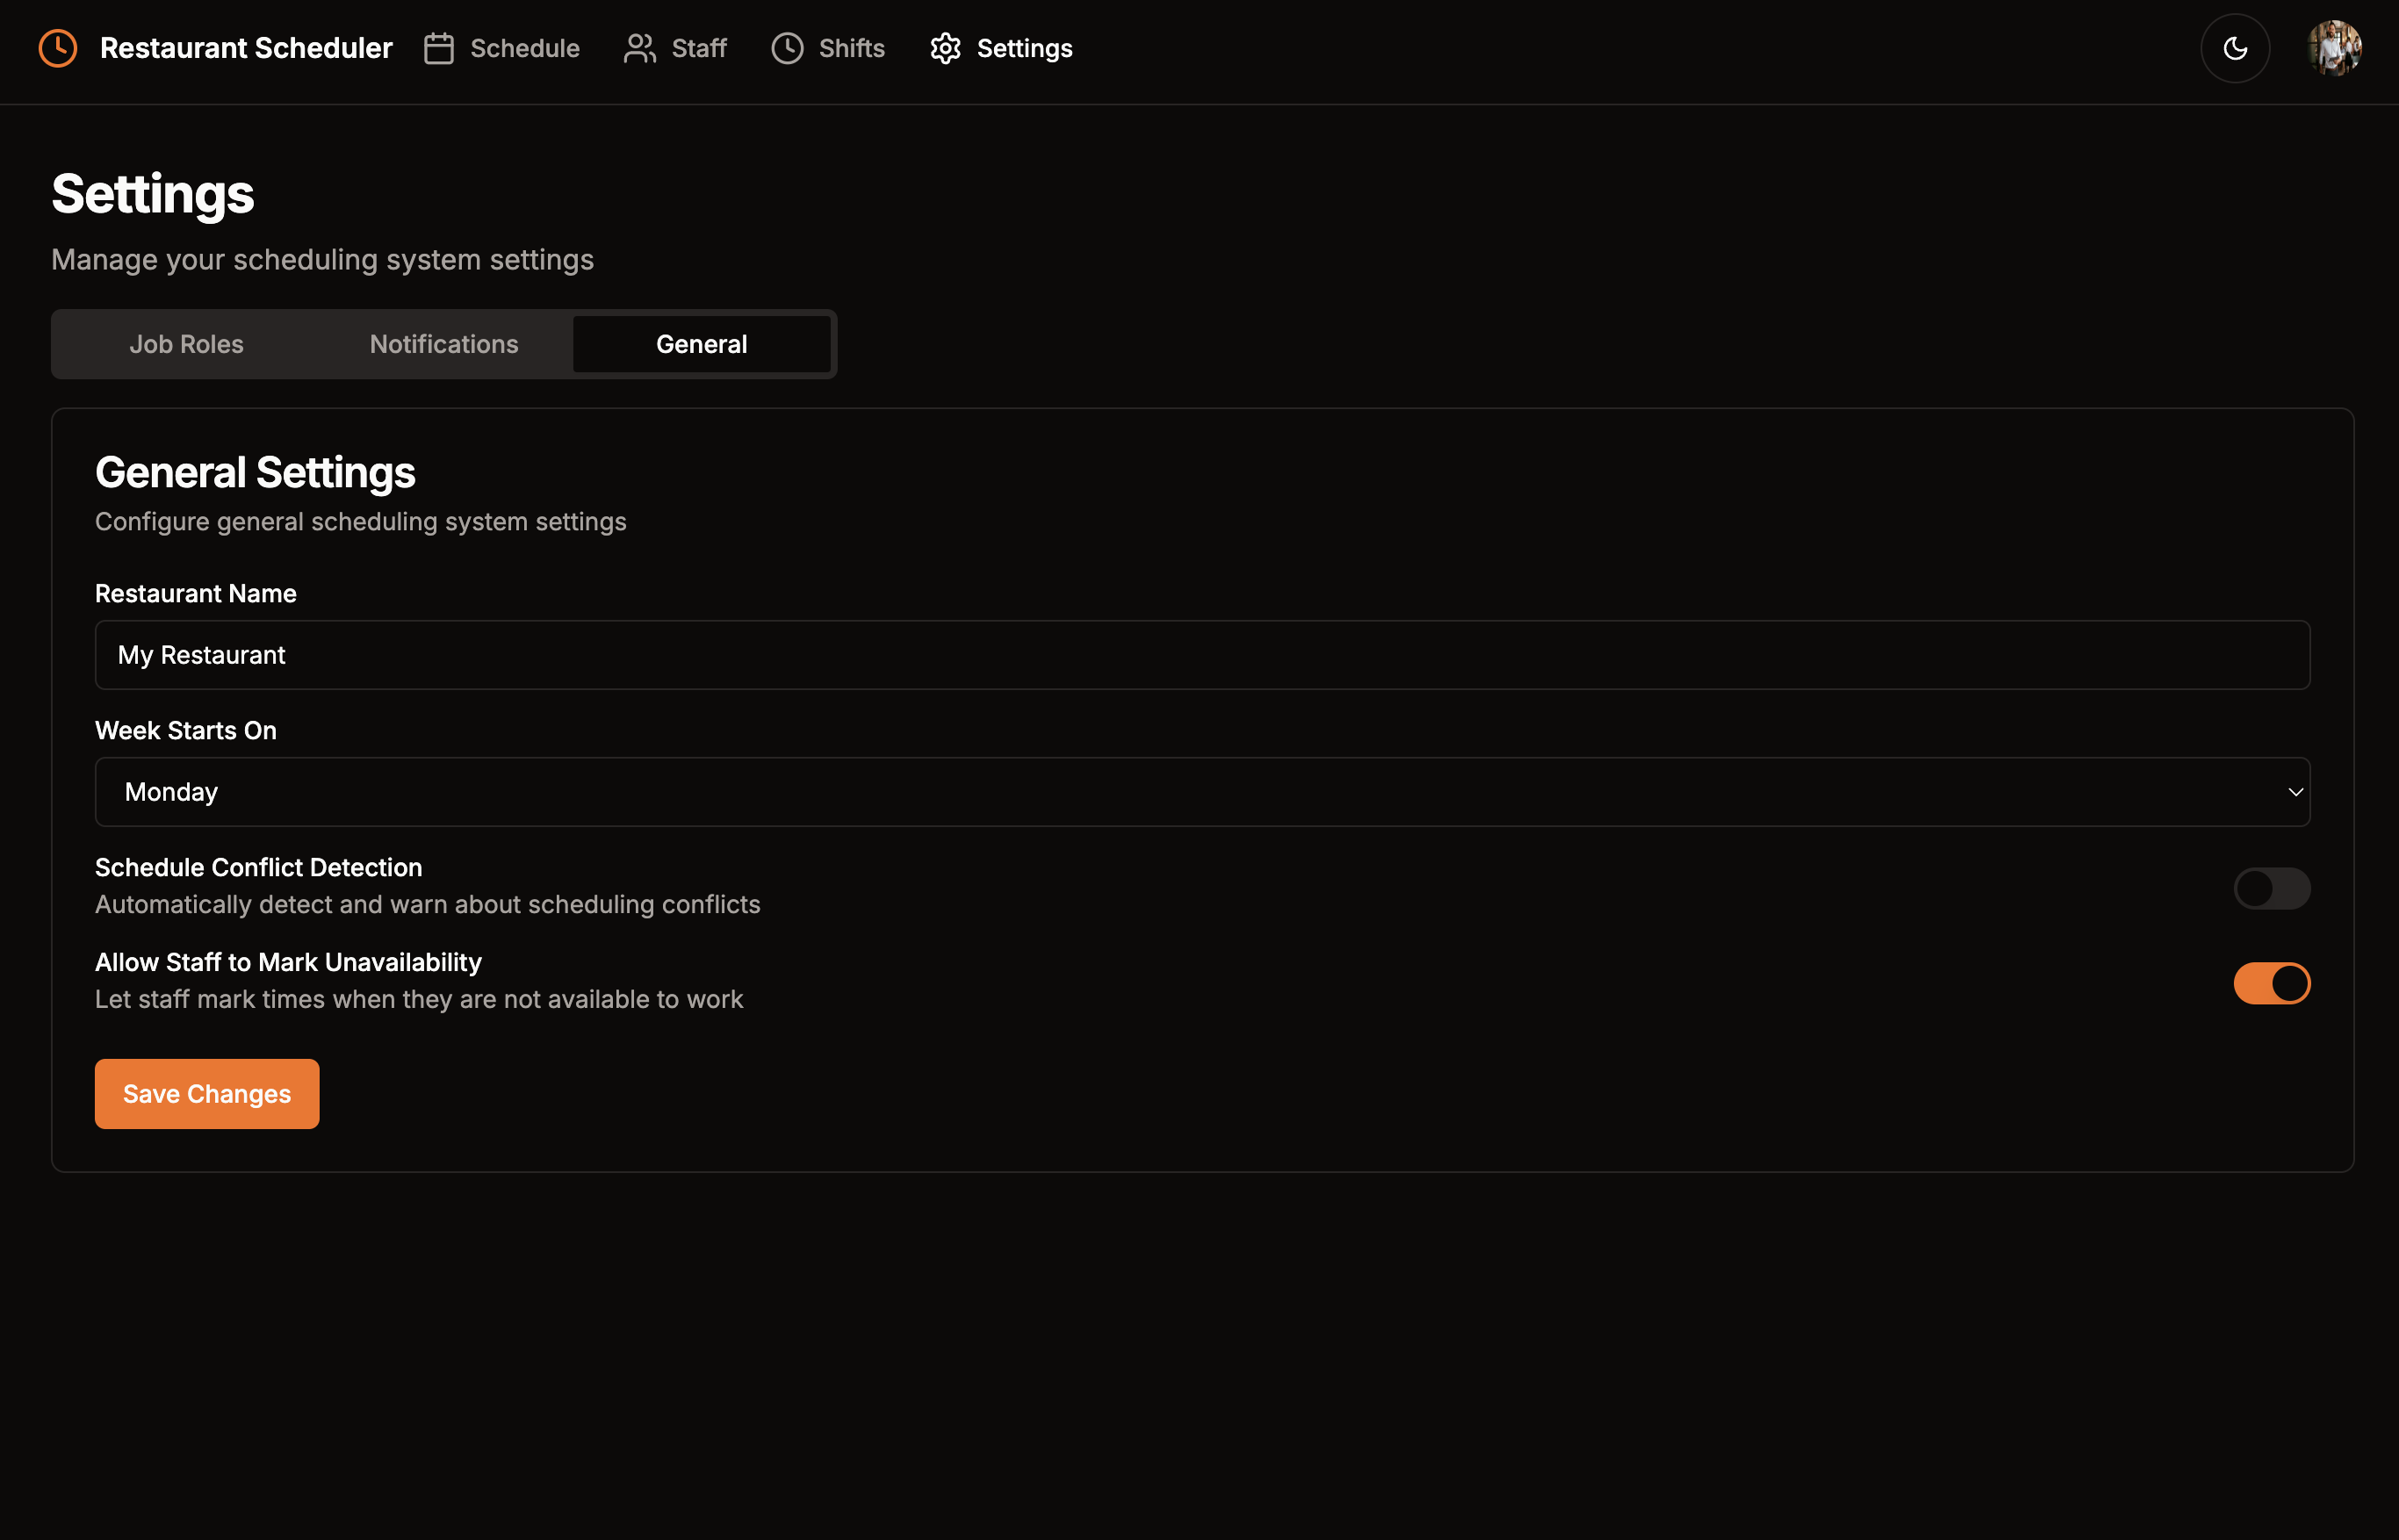
\includegraphics[width=15cm]{Sections/tong_quan/functional_spec/img/proto1.10.png}

     \vspace{0.5cm}
    \caption{Trang Settings (3)}
\end{figure}

\textbf{User Flow:}

\begin{figure}[H]
	\centering
	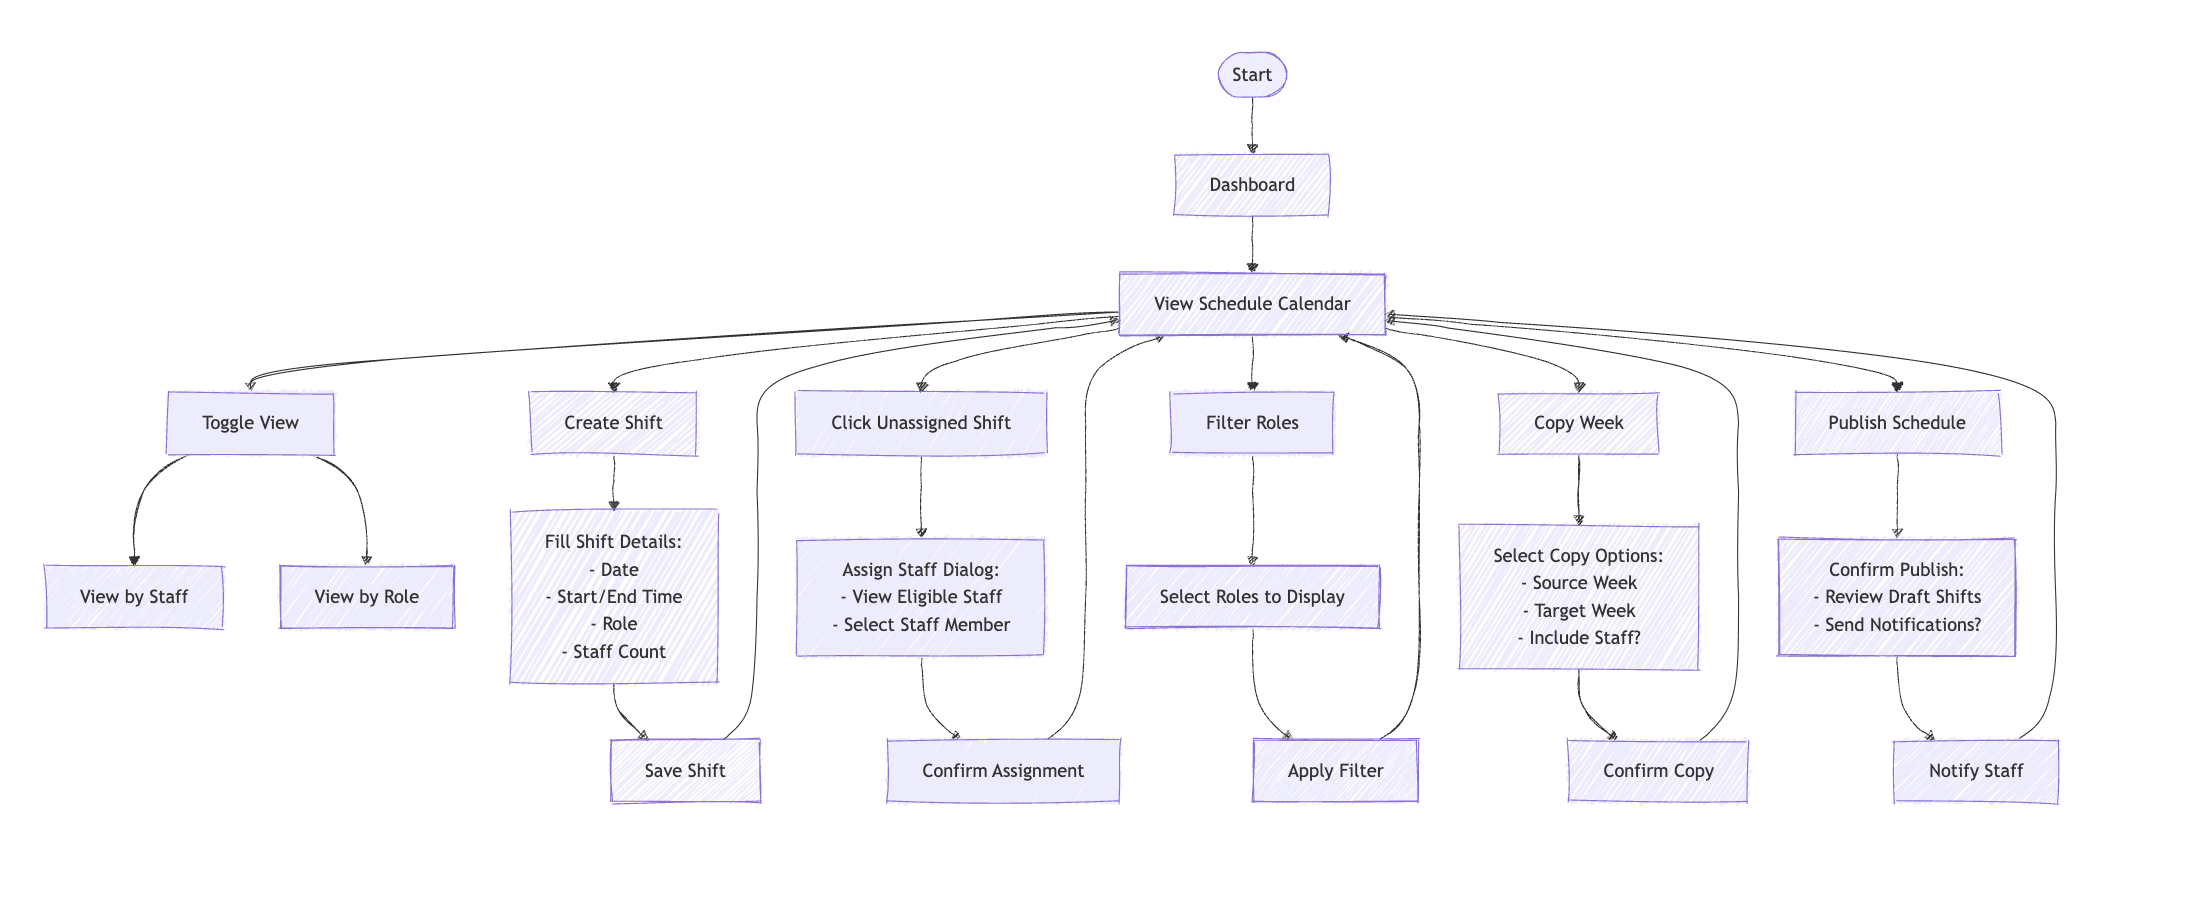
\includegraphics[width=15cm]{Sections/tong_quan/functional_spec/img/dashboard1.png}

     \vspace{0.5cm}
    \caption{User flow cho trang Dashboard}
\end{figure}
\begin{figure}[H]
	\centering
	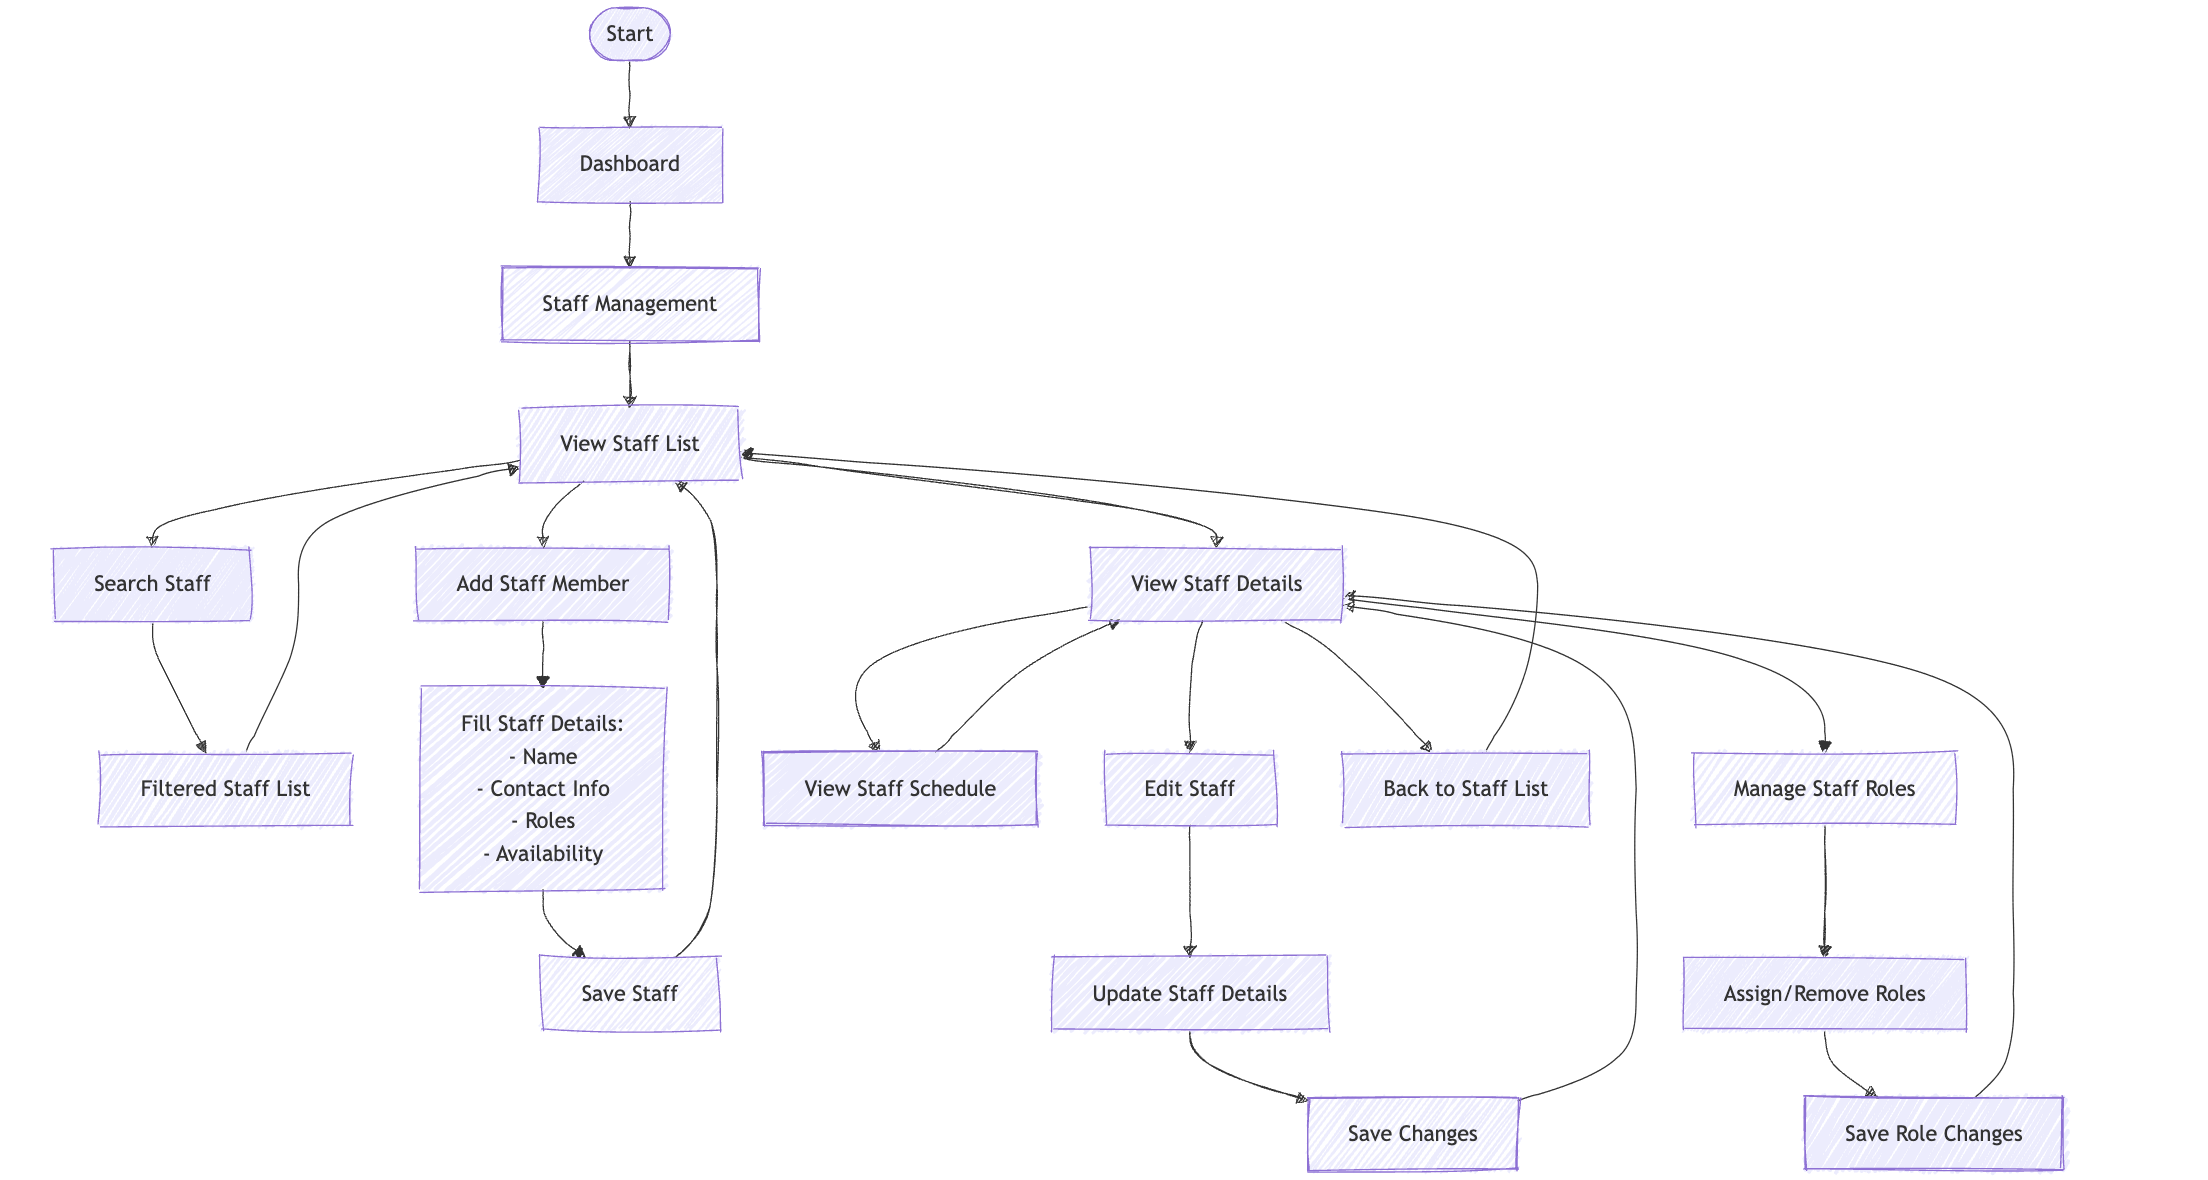
\includegraphics[width=15cm]{Sections/tong_quan/functional_spec/img/staffmanage1.png}

     \vspace{0.5cm}
    \caption{User flow cho trang Staff Management}
\end{figure}
\begin{figure}[H]
	\centering
	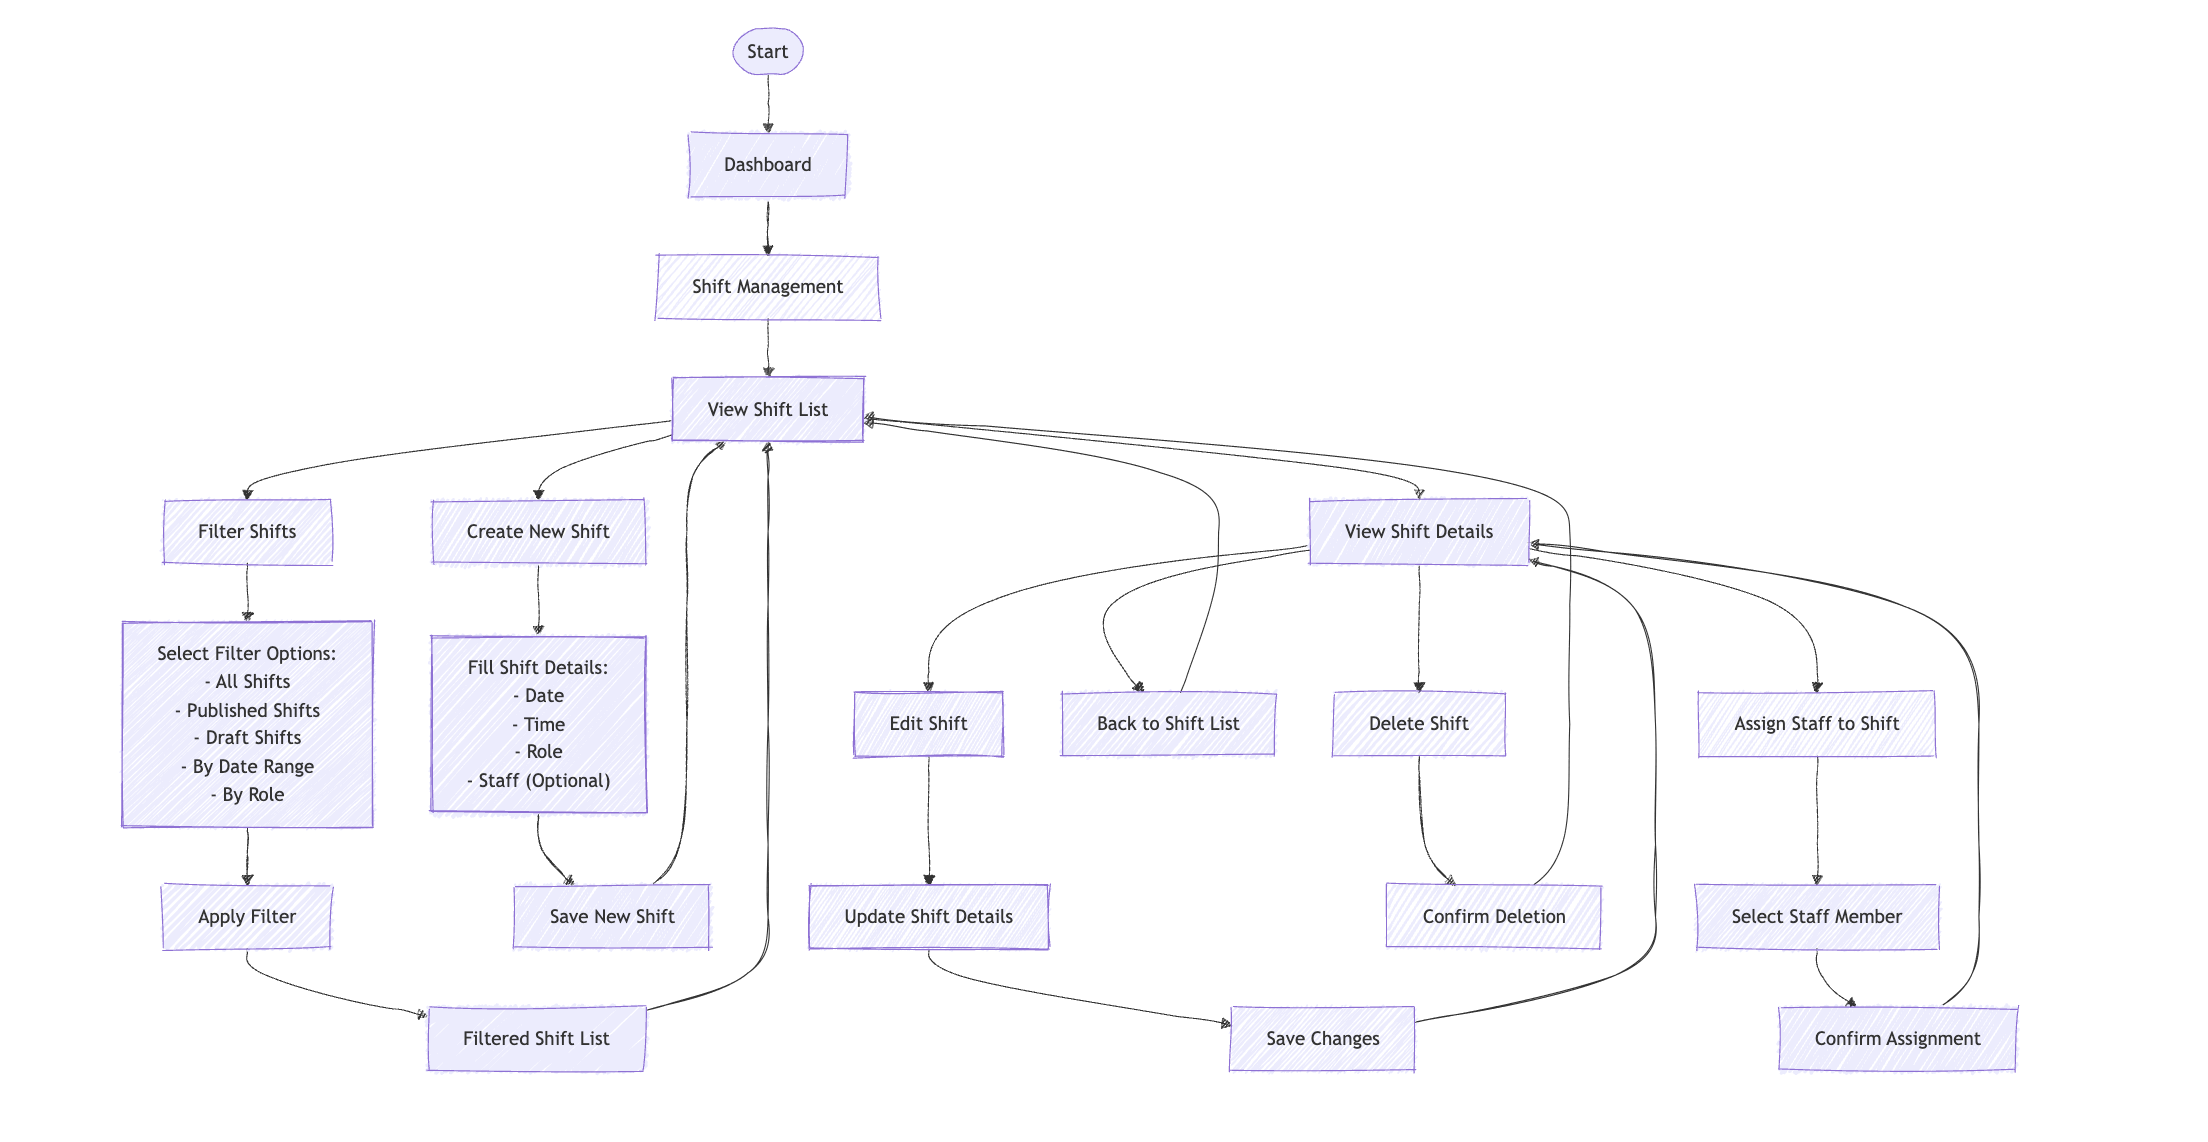
\includegraphics[width=15cm]{Sections/tong_quan/functional_spec/img/shiftmanage1.png}

     \vspace{0.5cm}
    \caption{User flow cho trang Staff Management}
\end{figure}
\begin{figure}[H]
	\centering
	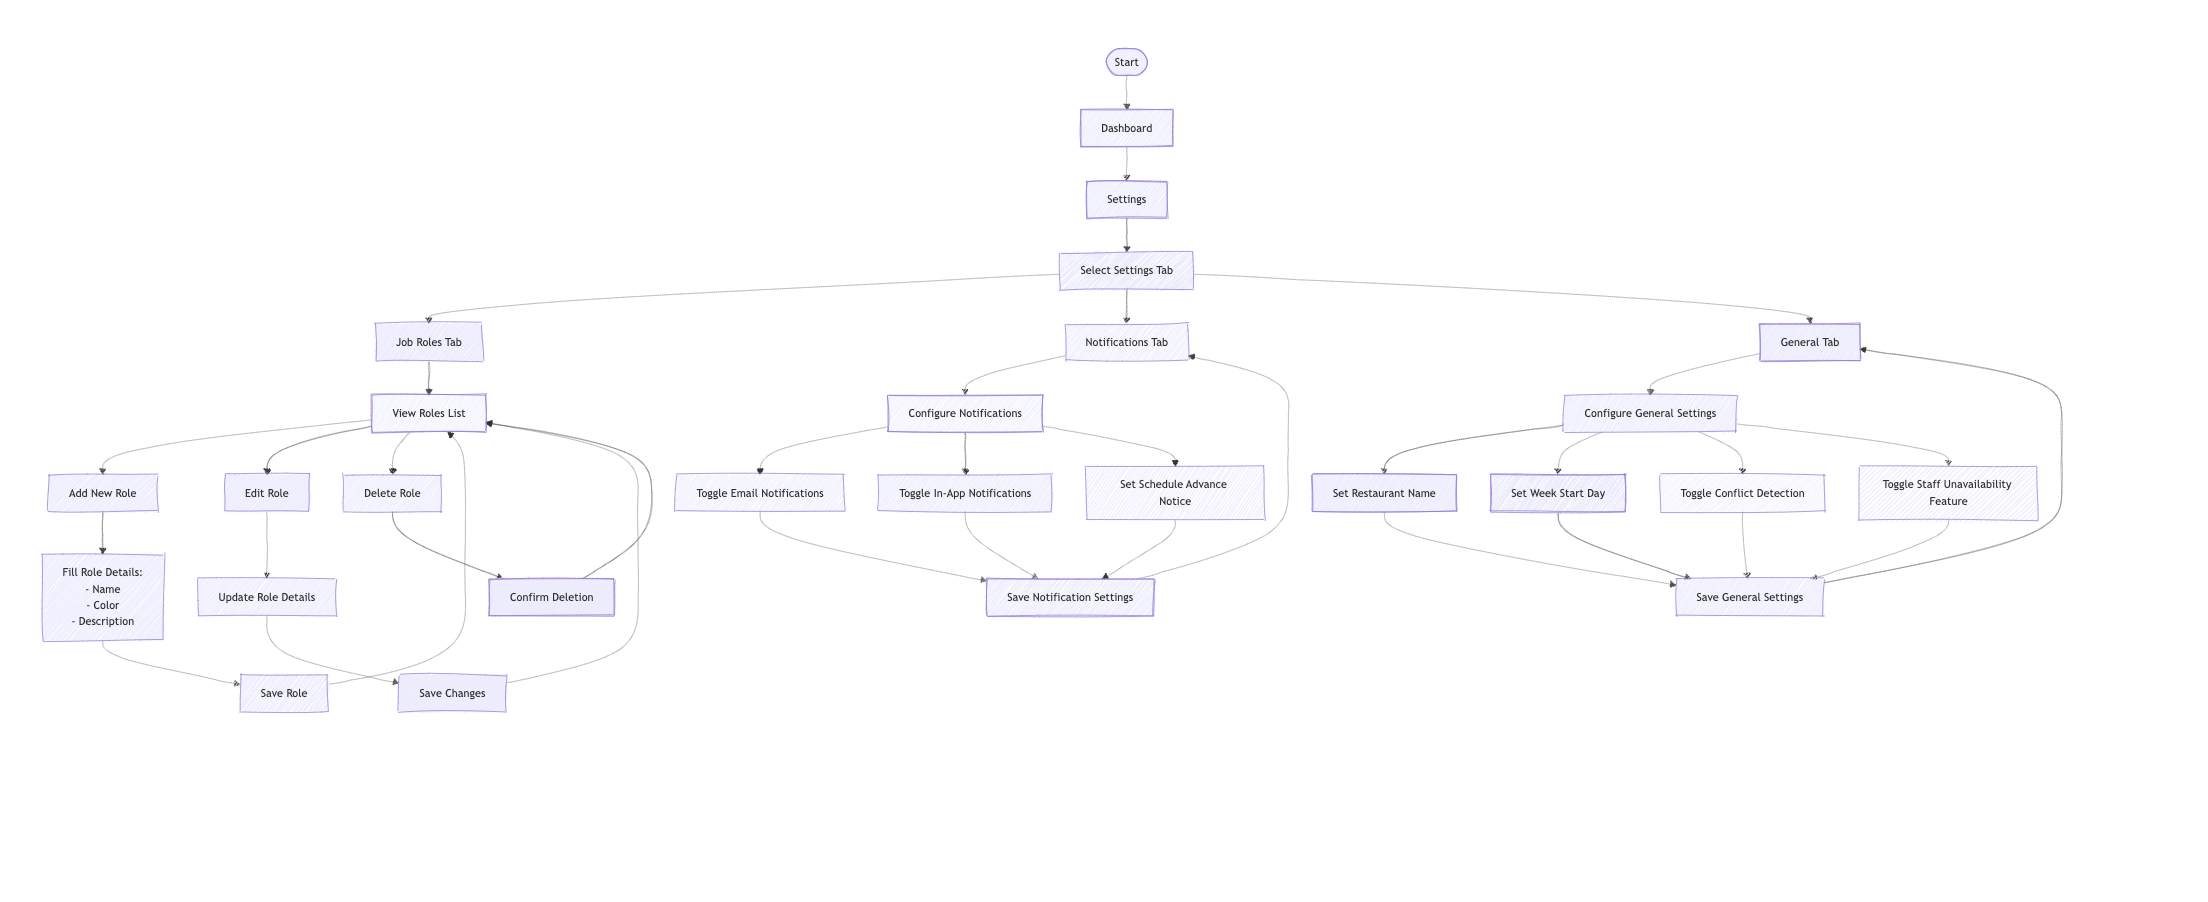
\includegraphics[width=15cm]{Sections/tong_quan/functional_spec/img/setting1.png}

     \vspace{0.5cm}
    \caption{User flow cho trang Settings}
\end{figure}